\documentclass[12pt]{article}
\usepackage[utf8x]{inputenc}
\usepackage{amsmath}
\usepackage{multicol}
\usepackage{graphicx}
\usepackage{float}
\usepackage{dsfont}
\usepackage{textcomp}
\usepackage{multirow}
\usepackage{amsfonts}
\usepackage{cleveref}
\usepackage{fancyhdr}
\setlength{\headheight}{14.5pt}
\renewcommand{\sectionmark}[1]{\markright{#1}{}}
\usepackage[T1]{fontenc}
\usepackage[colorinlistoftodos]{todonotes}
\usepackage[margin=2cm,a4paper]{geometry}
\newgeometry{left=2.0cm,right=2.0cm,top=2.5cm,bottom=2.5cm}
\usepackage{listings}
\setlength{\marginparwidth}{2cm}
\setlength{\parindent}{0pt}
\newcommand{\deriv}{\mathrm{d}}
\lstset{
    language=R,
    basicstyle=\scriptsize\ttfamily,
    commentstyle=\ttfamily\color{red},
    numbers=left,
    numberstyle=\ttfamily\color{blue}\footnotesize,
    stepnumber=1,
    numbersep=5pt,
    backgroundcolor=\color{white},
    showspaces=false,
    showstringspaces=false,
    showtabs=false,
    frame=single,
    tabsize=2,
    captionpos=b,
    breaklines=true,
    breakatwhitespace=false,
    title=\lstname,
    escapeinside={},
    keywordstyle={},
    morekeywords={}
    }
\title{}
\pagestyle{fancy}
\fancyhf{}
\rhead{\leftmark}
\lhead{Gamma-Ray Spectroscopy}
\lfoot{PH617 Physics Project Laboratory}
\rfoot{Page \thepage}
\renewcommand{\headrulewidth}{1pt}
\renewcommand{\footrulewidth}{1pt}
\begin{document}
\begin{titlepage}
\newgeometry{left=1.0in,right=1.0in,top=2.0in,bottom=2.0in}
\newcommand{\HRule}{\rule{\linewidth}{0.5mm}}
\begin{centering} 
%---------------------------------------------------------------------------
%	HEADING SECTIONS
%---------------------------------------------------------------------------

\includegraphics[scale=0.7]{Images/Uni_of_Kent.png}\\[1cm]
%---------------------------------------------------------------------------
%	TITLE SECTION
%---------------------------------------------------------------------------
\HRule \\ [0.3cm]
\Huge{\bfseries{Gamma Ray Spectroscopy}} \\
\textsc{\large PH617: Physics Project Laboratory}\\ [-0.1cm]
\textsc{\large Astronomy, Space Science and Astrophysics}\\ [-0.2cm]
\HRule \\[0.5cm]
%---------------------------------------------------------------------------
%	AUTHOR SECTION
%---------------------------------------------------------------------------
\begin{minipage}{0.625\textwidth}
\begin{center} \large
{\large Date: 2nd Oct 2020 - 2nd Nov 2020}\\[0.2cm]
{\large Report Author: Lukasz R Tomaszewski}\\[0.2cm]
{\large Word Count: 1713}\\
\end{center}
\end{minipage}\\[2cm]
\vfill
\end{centering} 
\end{titlepage}
%---------------------------------------------------------------------------
%	CONTENTS   
%---------------------------------------------------------------------------
\newpage
\begin{titlepage}
\begin{tableofcontents}
\end{tableofcontents}
\end{titlepage}
\newpage
%---------------------------------------------------------------------------
%	ABSTRACT
%---------------------------------------------------------------------------
\section{Abstract}
\label{Abstract Section}

As an excited nucleus encounters decay, that excess decay is transmitted via a gamma ray and when directed towards a detector that measures its counts can be used to identify the nucleus, Utilizing two radioactive sources (Cobalt and Cesium) the measurement of their gamma ray count that penetrated different thicknesses of Lead and Aluminium can also determine their absorption rate which is dependant of the material. The aim is to determine which material is better at absorbing gamma rays and determine what source the gamma rays come from by measuring the count. It’s to be shown that Lead absorbs gamma rays more than Aluminium thus making Lead a good shielding material to contain and or stop gamma rays penetrating through. Though these count, the energy resolution of the spectrometer is calculated as the activity of the radioactive sources are measured, thus the linear and mass attenuation co-efficient are calculated at different energies that determine the radioactive source.

%---------------------------------------------------------------------------
%	INTRODUCTION
%---------------------------------------------------------------------------
\section{Introduction}
\label{Introduction Section}

Within this experiment, the aims will be to observe gamma-ray spectroscopy through the rays ability to penetrate through not only different materials but different thicknesses of materials. Using various thicknesses (ranging from 1-10mm) of the materials (Lead and Aluminium), a count of gamma rays that penetrated the material are measured from a detector where the materials were placed in between the radioactive sources (Cobalt and Cesium) and the detector. When a excited nucleus encounters decay, the excess energy of that decay is transmitted via a gamma ray, this energy is converted into voltage by a spectrometer as well as measures the amount of photons being produced from the gamma rays. \\ [0.4cm]
Utilizing the the total counts of each peak in the 6 different spectra presented, the intensity of the gamma radiation emitted by the radioactive source can be compared to the energy of each photon that not only allows us to observe how gamma radiation interacts with different nuclei but also to determine which material is better at containing these radioactive elements so that the harmful radiation does not harm us as human beings. \\

The aims are to create an experiment and observe this and to; \cite{Exp.C-2020}
\begin{itemize}
    \item Understand $\gamma$-ray spectroscopy and detectors.
    \item Identify key features on an energy spectrum.
    \item Find energy resolution of the spectrometer.
    \item Measure activity of radioactive sources.
    \item Find the linear attenuation co-efficient for lead and aluminium at different energies.
    \item Find the mass attenuation co-efficient for lead and aluminium at different energies.
\end{itemize}

%---------------------------------------------------------------------------
%	METHODOLOGY
%---------------------------------------------------------------------------
\section{Methodology}
\label{Methodology Section}
%---------------------------------------------------------------------------
\subsection{Experimental Setup}
\label{Experimental Setup Subsection}
  
Connecting the detector to voltage box and then to the computer (CASSY software) and suspending the Cobalt/ Cesium on clamp above the detector with a tray that holds the materials of lead and aluminium in between them both, shown in \cref{Setup of Apparatus}. The radioactive material (Cobalt and Cesium) are centred by eye directly above the detectors, no accurate form of centering was available due to health and safety that the radioactive sources must face down at all times to avoid directing the gamma-rays towards the operator.

\begin{figure}[H]
\centering
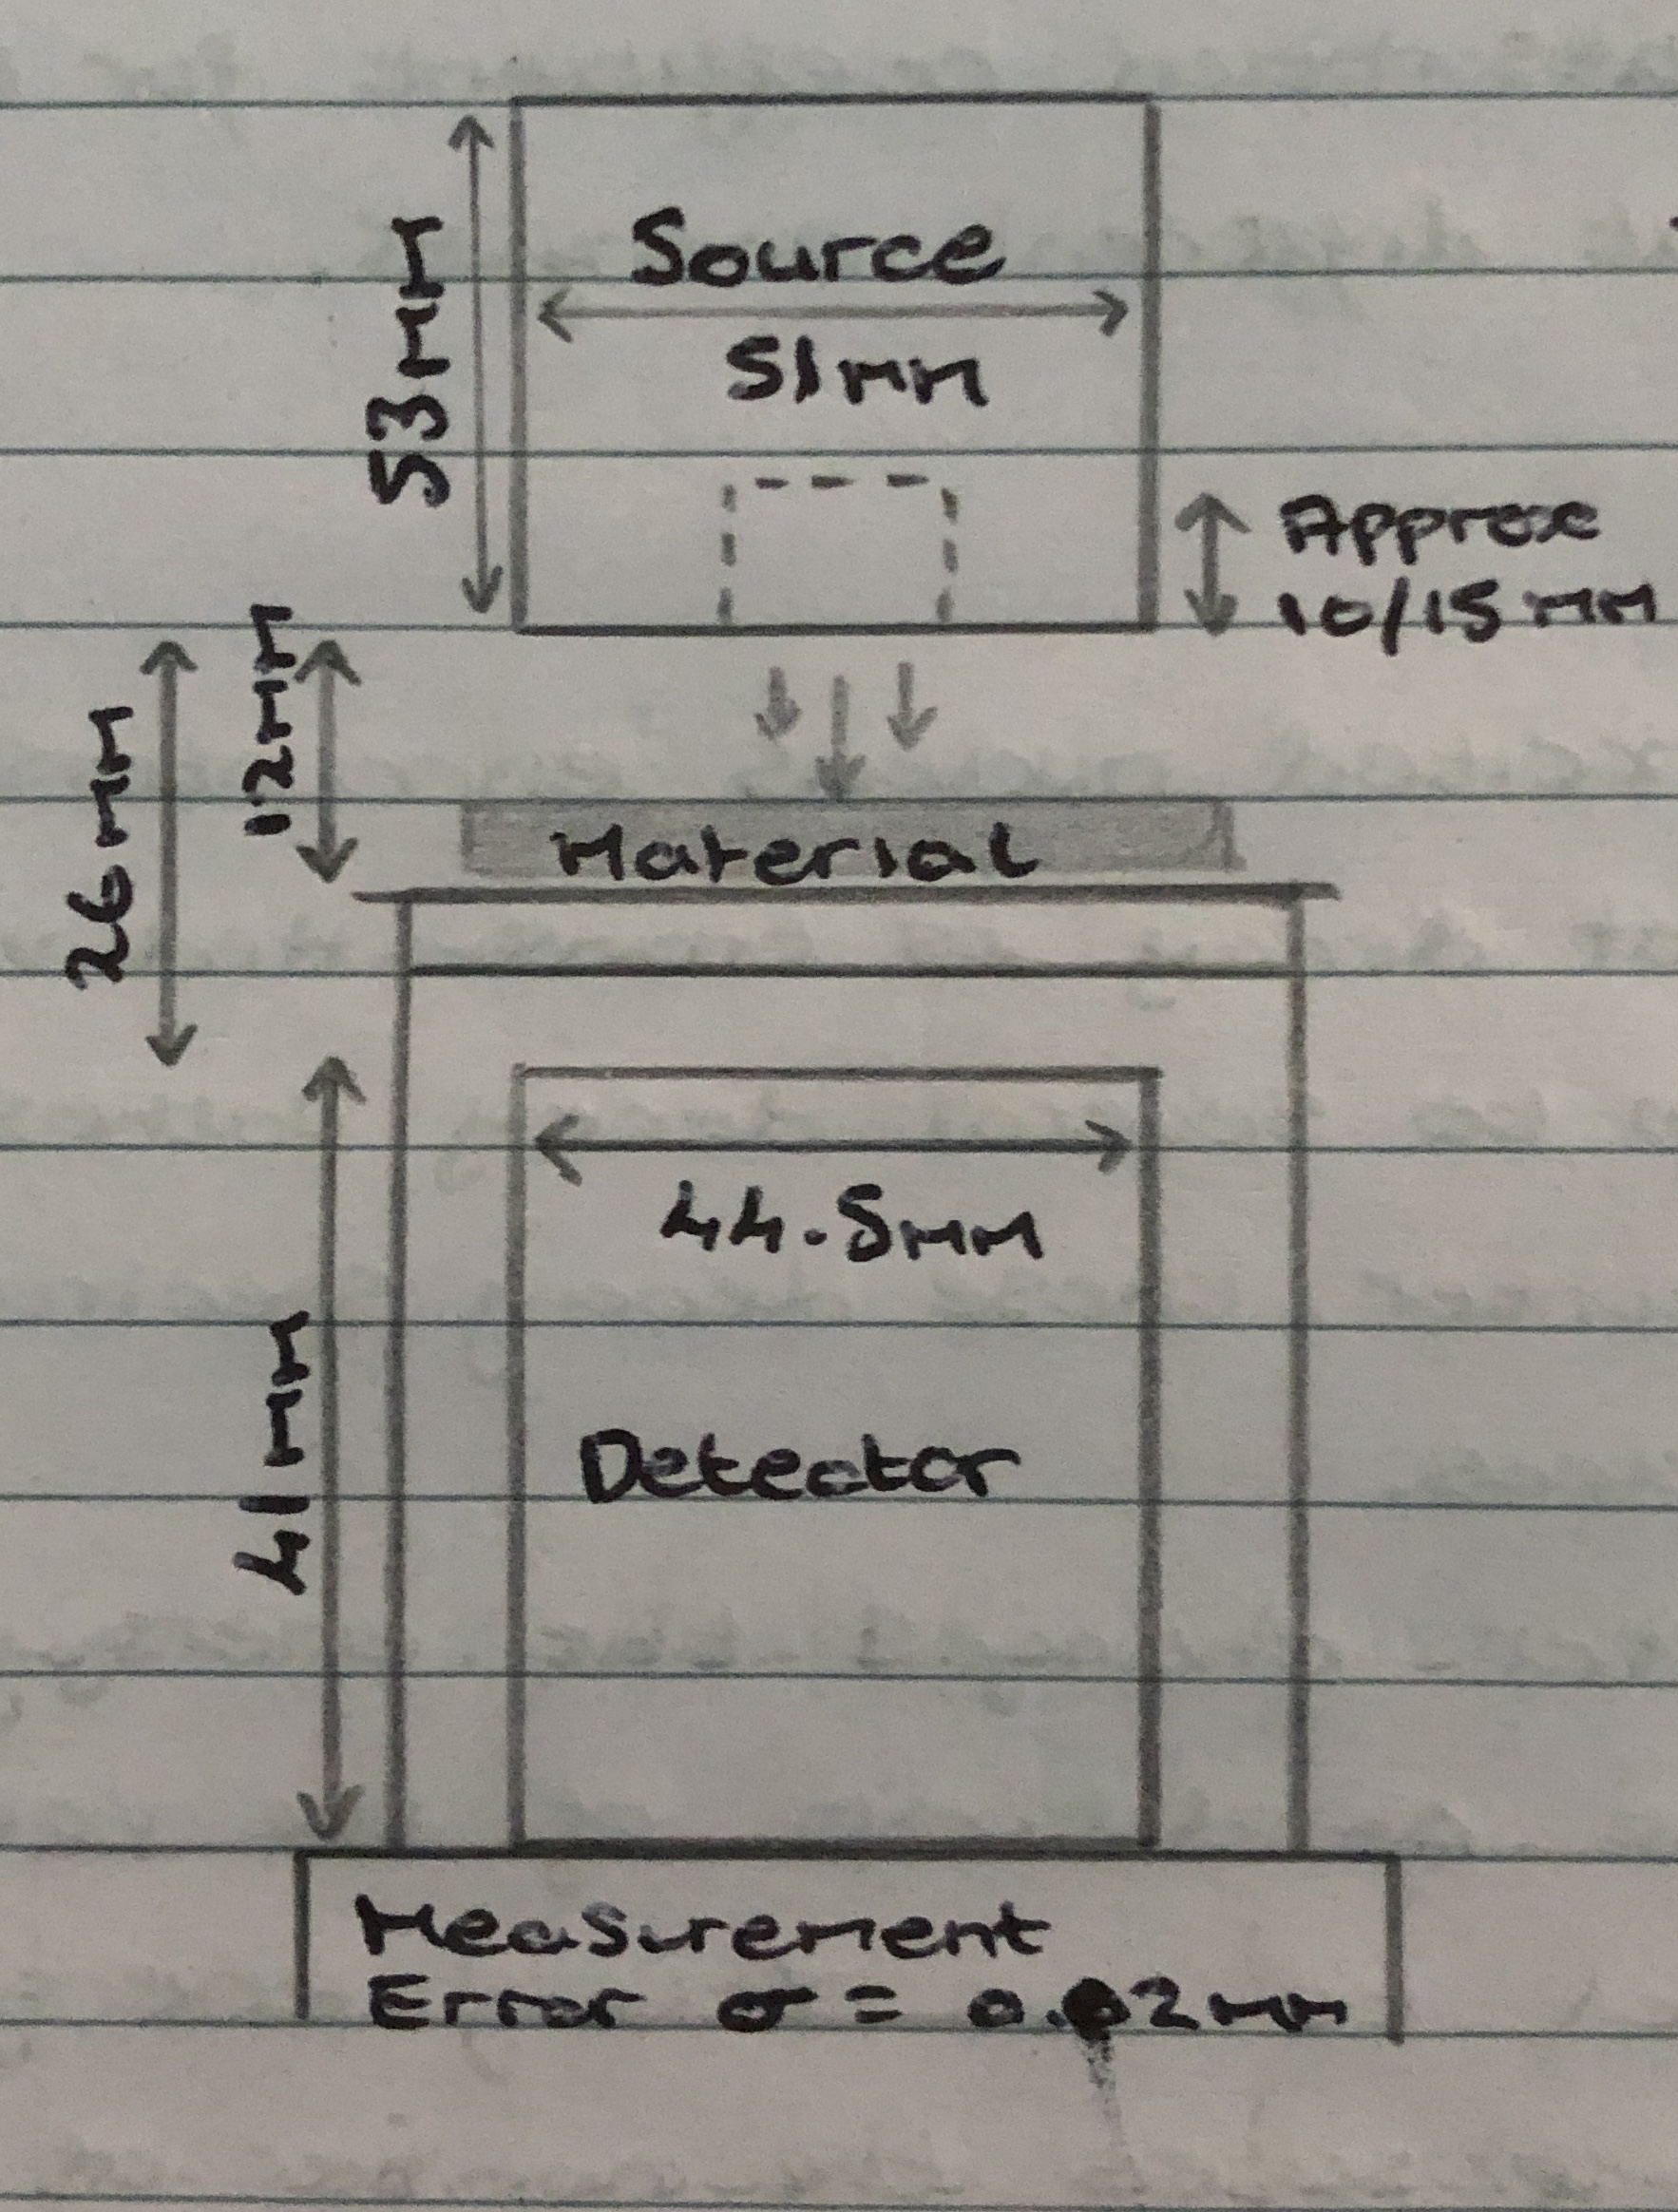
\includegraphics[scale=0.12]{Images/IMG_0338.jpg}
\caption{Setup and measurements of the radioactive material over the detector \cite{Exp.C-Lab_book}}
\label{Setup of Apparatus}
\end{figure}

The experiment begins with calibration of the apparatus so that we have a reference point specified in \cref{Energy Calibration SubSection}. Setting up Cassy to the following parameters \cite{Exp.C-2020} after which CASSY is ready to begin recording the desired measurements:\\
\begin{itemize}
    \item No. of channels is set to 512
    \item Integration time is set to 300s
    \item Check gain box A1 is set to -2
    \item Negative pulse is ticked
    \item Check pulse height is -2500mV
\end{itemize}

%---------------------------------------------------------------------------
%	REPORT & FINDINGS
%---------------------------------------------------------------------------
\section{Results \& Findings}
\label{Results & Findings Section}

%---------------------------------------------------------------------------
\subsection{Energy Calibration}
\label{Energy Calibration SubSection}

\begin{table}[H]
\begin{center}
 \footnotesize
 \begin{tabular}{|c||c||c|c|c||c|c|}
 \hline
  $^{60}Cobalt$ & Compton Count & Peak Count & Peak(N1) & Peak $\sigma$ & Peak Energy (keV) & Peak Energy (keV) $\sigma$\\
 \hline 
  1.17 MeV & 25,155 & 1418 & 0.00192 & $\pm$0.5 & 1172.82 & $\pm$26.67 \\
 \hline
  1.33 MeV & 0.01248 & $\pm$0.000017 & 0.01196 & $\pm$0.00019 & 1.60815 & $\pm$0.00258 \\
 \hline \hline
  $^{137}Cesium$ & Compton Count & Peak Count & Peak(N1) & Peak $\sigma$ & Peak Energy (keV) & Peak Energy (keV) $\sigma$ \\
 \hline
 0.66 MeV & 0.01248 & $\pm$0.000017 & 0.01196 & $\pm$0.00019 & 1.60815 & $\pm$0.00258 \\
 \hline 
 \end{tabular} \\ 
 \caption{Data sourced from Cassy.}
 \label{Calibration Data}
\end{center}
\end{table}

Recording the data without the materials (Lead and Aluminium) in between the radioactive source and the detectors allows for a reference point to be sourced, following the lab script \cite{Exp.C-2020} and sourcing from CASSY the peak to peak area count for all the peaks and the Compton scattering effect peak and peak centres that is displayed in \cref{Calibration Data}. This allows us to see and target the energy levels for each source to their peaks. The large peak is the Compton scattering effect that defines the inelastic collisions between the photons and the loose electrons, when using the radioactive source Cobalt the left peak is associated with the energy 1.17 MeV and the right peak is associated 1.33 MeV whereas the only peak for Cesium is related to the energy level 0.66 MeV.

%---------------------------------------------------------------------------
\subsubsection{Energy resolution}
\label{Energy Resolution SubsubSection}

"The energy resolution is defined as the full width at half maximum of the photo-peak divided by the peak position" \cite{Exp.C-2020} thus the full width half maximum of the photo peaks of the energy levels 1.17 MeV, 1.33 MeV and 0.66 MeV. As stated, the FWHM is defined as:

\begin{equation}
E_R = \dfrac{FWHM (Peak)}{Peak (MeV)}
\label{ER Eq}
\end{equation} 

\begin{table}[H]
\begin{center}
 \footnotesize
 \begin{tabular}{|c||c|c|c|c|}
 \hline
  $^{60}Cobalt$ & FWHM & Peak Energy (keV) & Energy Resolution & $\sigma$ \\
 \hline 
  1.17 MeV & 18.1 & 1172.82 & 0.015 & $\pm$0.003 \\
 \hline
  1.33 MeV & 16.8 & 1328.99 & 0.013 & $\pm$0.006 \\
 \hline \hline
  $^{137}Cesium$ & FWHM & Peak Energy (keV) & Energy Resolution & $\sigma$ \\
 \hline
 0.66 MeV & 12.3 & 661.71 & 0.019 & $\pm$0.001 \\
 \hline 
 \end{tabular} \\ 
 \caption{Energy Resolution data calculated from using \cref{Calibration Data} and putting it through \cref{ER Eq}. }
 \label{ER Data}
\end{center}
\end{table}

%---------------------------------------------------------------------------
\subsubsection{Compton Scattering}
\label{Compton Scattering SubsubSection}

Calculating the amount of gamma rays lost due to the Compton scattering effect shows the amount of inelastic collisions that took place, this allows for more accurate results when targeting the desired energy levels in Cobalt (1.17MeV and 1.33MeV) and Cesium (0.66MeV). Its stated as the peak count over the Compton scatting effect count:

\begin{equation}
C_S = \dfrac{Peak Integral Count}{Compton Integral Count}
\label{CS Eq}
\end{equation} 

\begin{table}[H]
\begin{center}
 \footnotesize
 \begin{tabular}{|c||c|c|c|c|}
 \hline
  $^{60}Cobalt$ & Compton Integral & Peak Integral & Compton $\gamma$-ray lost & $\sigma$ \\
 \hline 
  1.17 MeV & 25155 & 1418 & 0.0564 & $\pm$0.0004 \\
 \hline
  1.33 MeV & 25155 & 1155 & 0.0459 & $\pm$0.0009 \\
  \hline
  Combined & 25155 & 2573 & 0.1023 & $\pm$0.0003 \\
 \hline \hline
  $^{137}Cesium$& Compton Integral & Peak Integral & Compton $\gamma$-ray lost & $\sigma$ \\
 \hline
 0.66 MeV & 224220 & 106899 & 0.4768 & $\pm$0.0007 \\
 \hline 
 \end{tabular} \\ 
 \caption{Compton scattering data calculated from using \cref{Calibration Data} and putting it through \cref{CS Eq}. }
 \label{ER Data}
\end{center}
\end{table}

%---------------------------------------------------------------------------
\subsection{Relative Strength}
\label{rrelative Strength SubSection}

To determine the relative strength, the absolute measure must be calculated first which is the absolute total count that could hit the detector its defined as "absolute measure is the area of the source and detector over a solid angle of $4\pi$ steradians". In \cref{detector} shows the spherical behaviour of the gamma rays as they leave the radioactive source and hit the detector. Using values measured in \cref{Setup of Apparatus} where D = 0.0445m and r-h = 0.026m. \\

\begin{figure}[H]
\centering
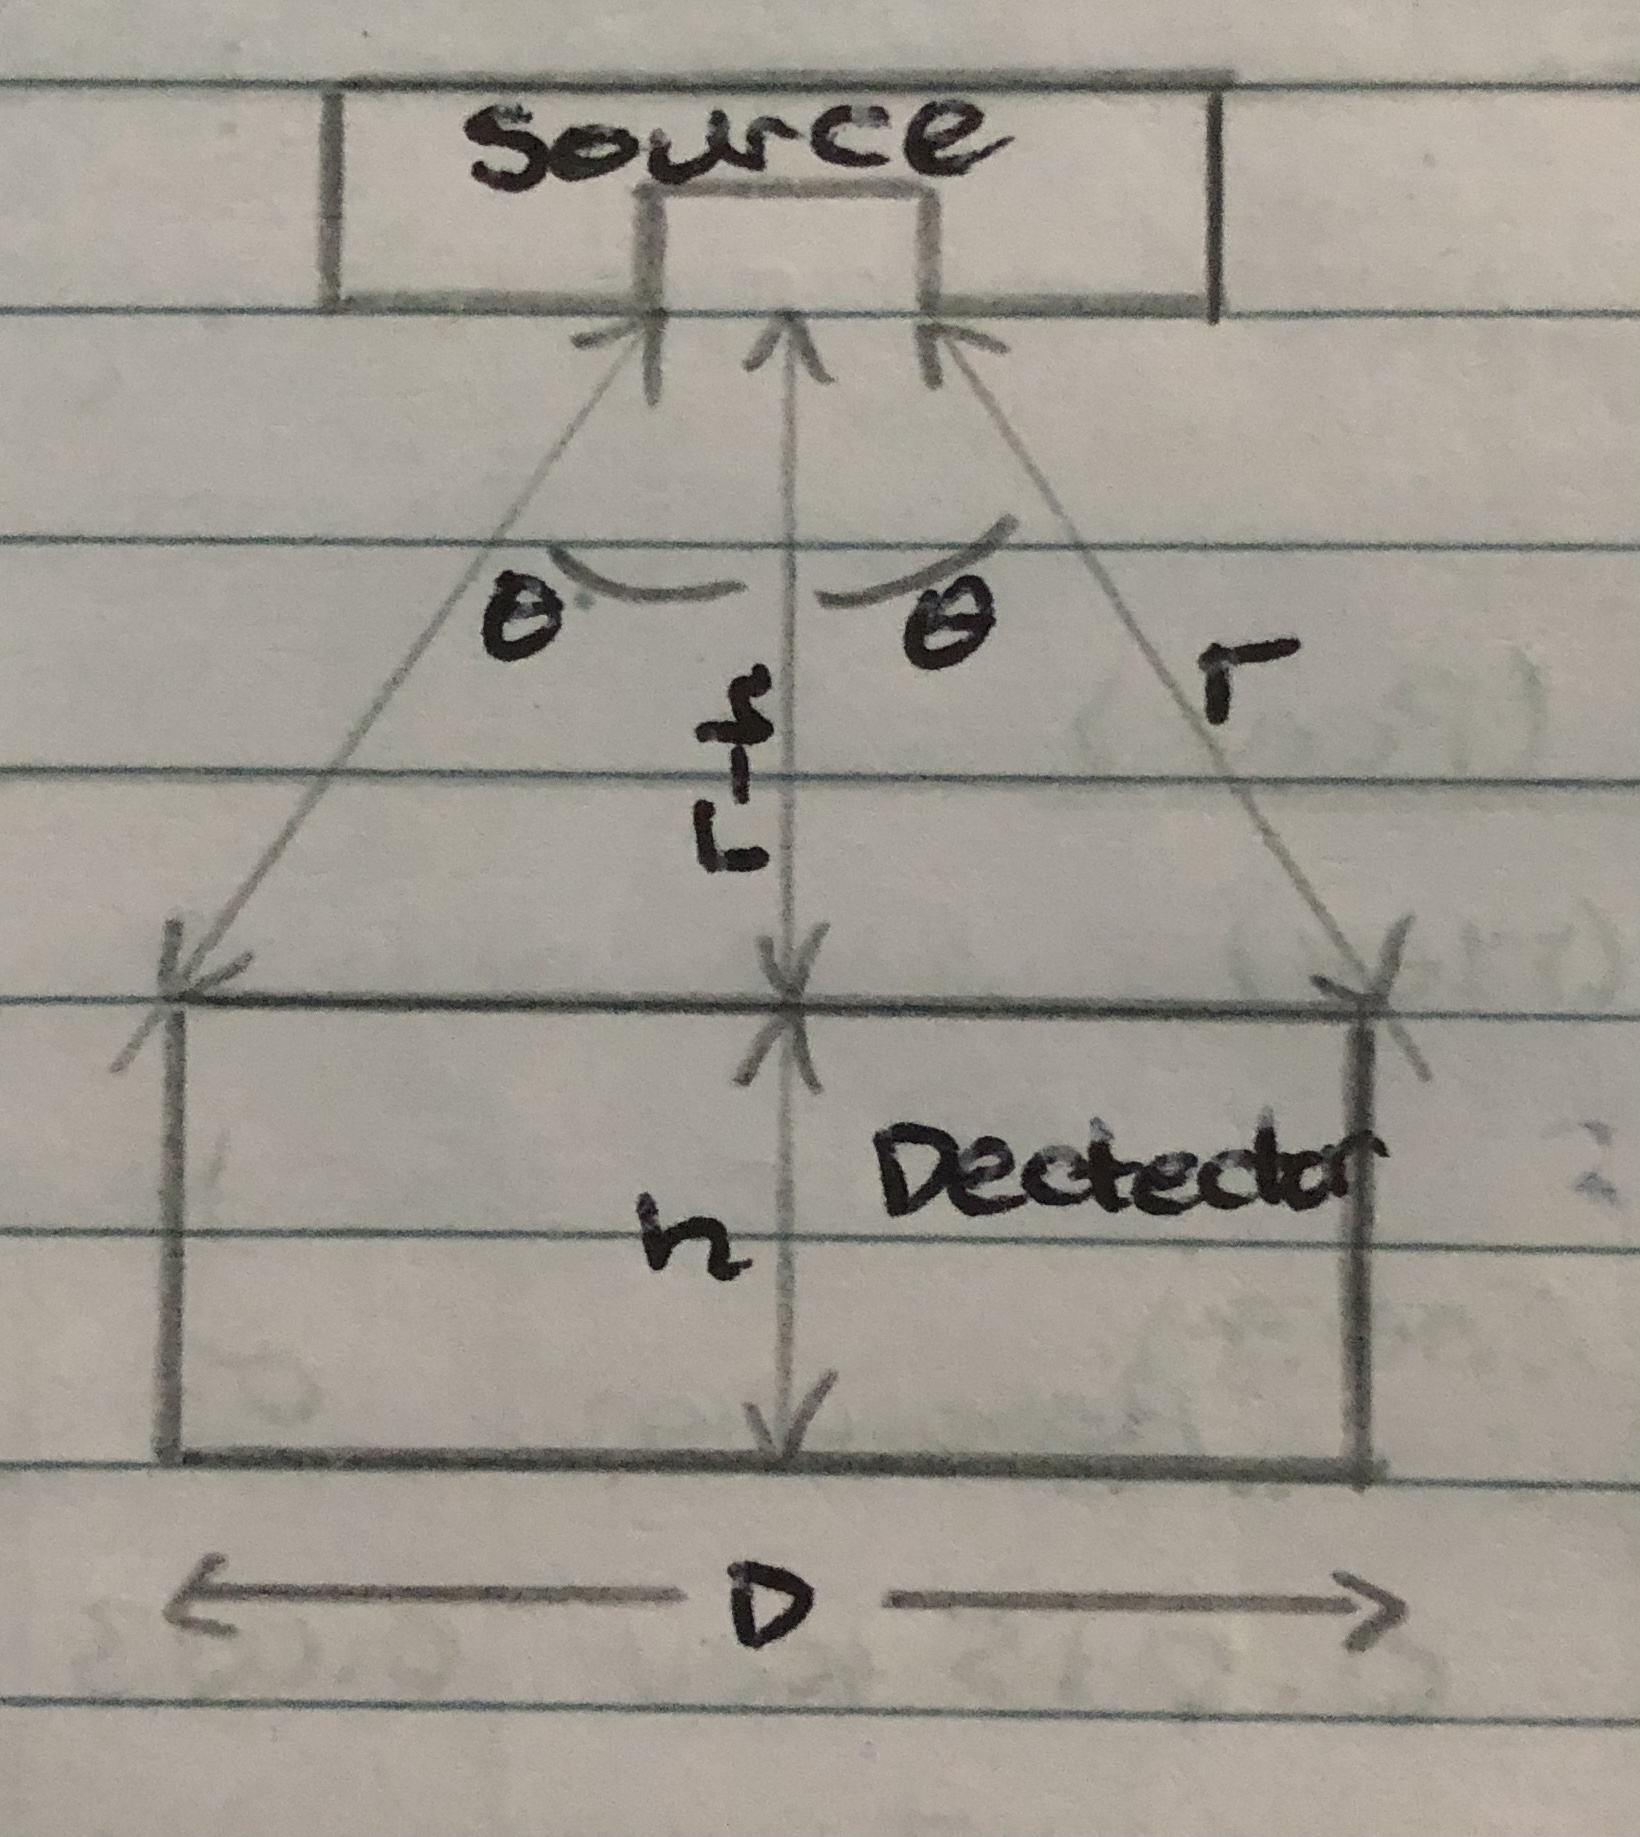
\includegraphics[scale=0.12]{Images/IMG_0339.jpg}
\caption{Graphical representation the sphere of gamma radiation direction around the detector.}
\label{detector}
\end{figure}

Using trigonometry and the law of solid angles r = 0.05242m and $\theta$=1.051 radians. And the Area of the source and the detector are calculated in \cref{A1 Eq} and \cref{A2 Eq} respectively.\\

\begin{equation}
A_1 = Source = \dfrac{r\theta}{4\pi} 
\label{A1 Eq}
\end{equation} 

\begin{equation}
A_2 = Source = \dfrac{r^2}{4\pi} 
\label{A2 Eq}
\end{equation} 

These equations output the $A_1$=0.00438$m^2$ and $A_2$=0.000219$m^2$, which then can be inputted in \cref{AM Eq} which takes into account the count per seconds where the total counts are used from \cref{Calibration Data}.\\

\begin{equation}
A_M = \dfrac{\dfrac{A_1}{A_2}* Total Counts}{Time}
\label{AM Eq}
\end{equation} 

\cref{AM Eq} outputs $AM_{Cobalt}$ = 1848.53 and $AM_{Cesium}$ = 22,074.6 \\

The relative strength is calculated as one source over the other, so the relative strength of Cobalt is the absolute measure of Cobalt over Cesium and the relative strength of Cesium is the absolute measure of Cesium over Cobalt.\\

So:
\begin{equation}
RS_{Cesium} = 0.0837 \pm0.001
\label{RSCO Eq}
\end{equation}
\begin{equation}
RS_{Cesium} = 11.9417 \pm0.001
\label{RSCE Eq}
\end{equation}

%---------------------------------------------------------------------------
\subsection{Absorption of $\gamma$-rays in matter.}
\label{Absorption SubSection}

Performing a series of measurements with CASSY where there is placed between the radioactive source and the detector various thicknesses of Lead and Aluminium and the graphs above show. Plotting all the thicknesses against each other while segregation the different materials and including graphs of the original count and the energy level vs counts allows for further analysis n how various thicknesses of materials interfere with the gamma rays penetration.\\


\begin{multicols}{2}
\begin{figure}[H]
\centering
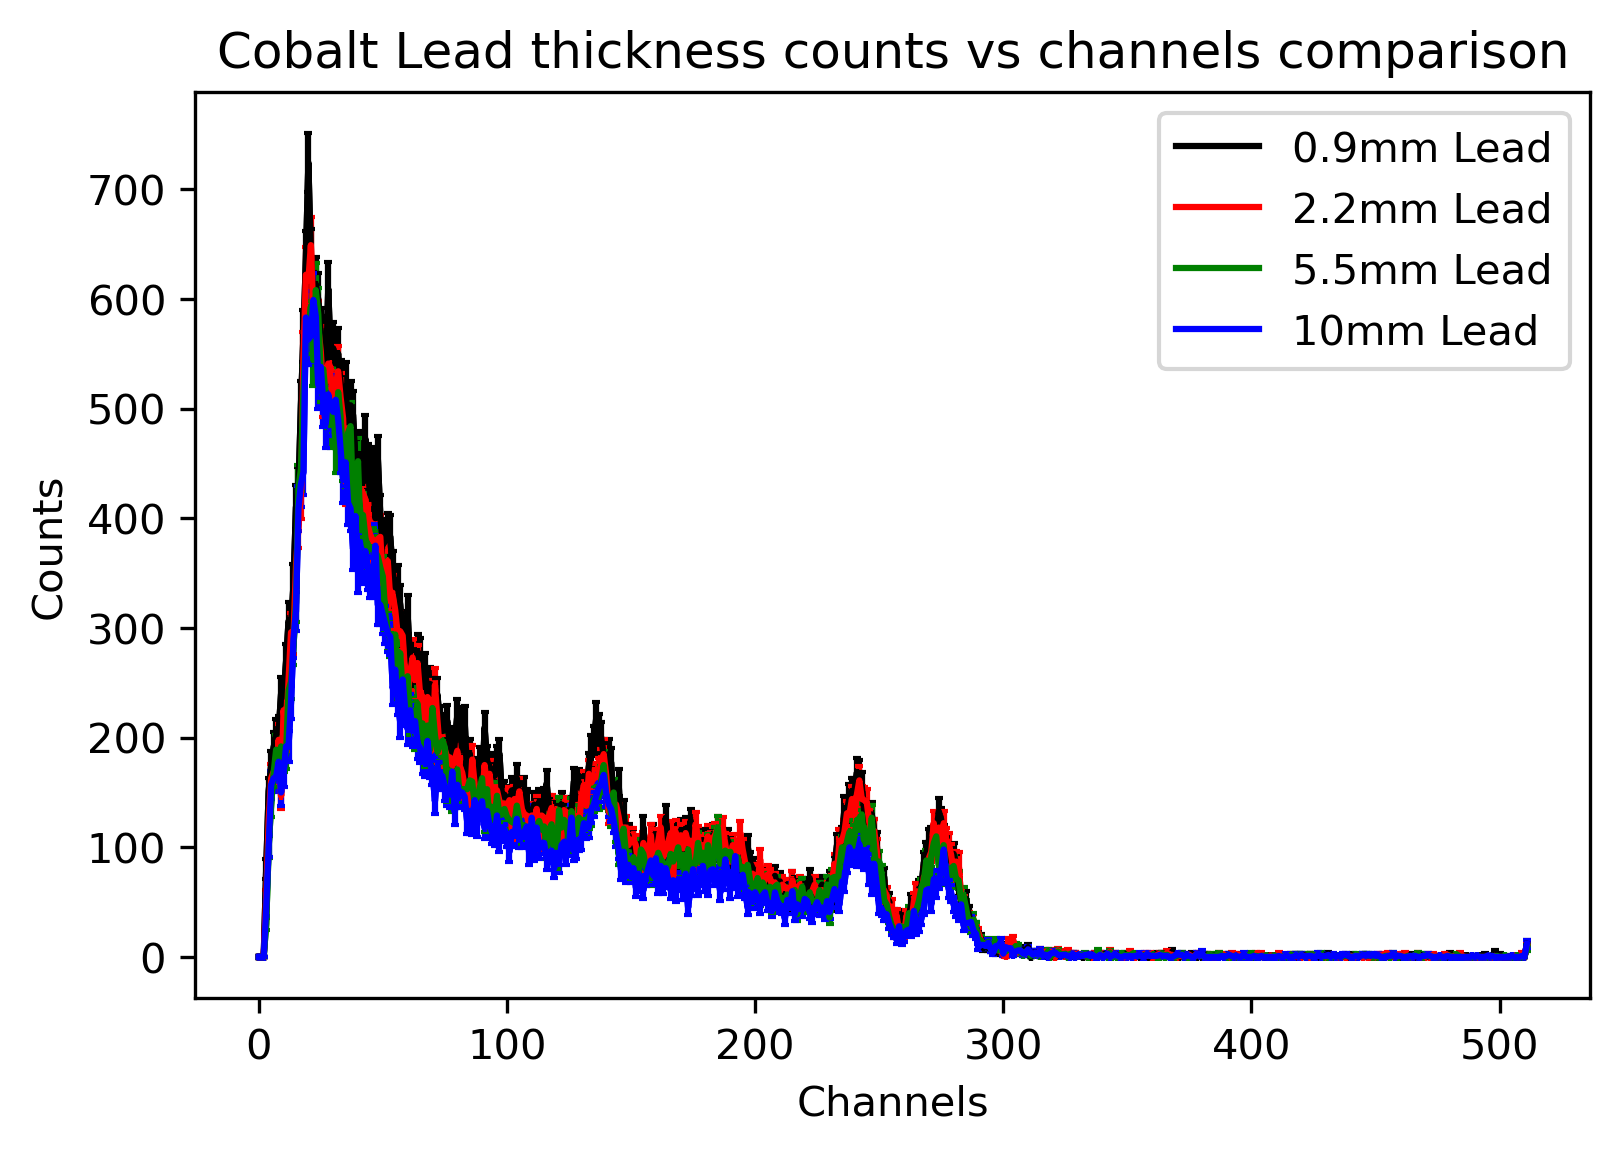
\includegraphics[scale=0.6]{Images/CobaltLeadCounts.png}
\caption{Graphical representation of raw data sourced from Cassy showing Lead thickness counts of Cobalt.}
\label{Cobalt Lead Counts}
\end{figure}

\begin{figure}[H]
\centering
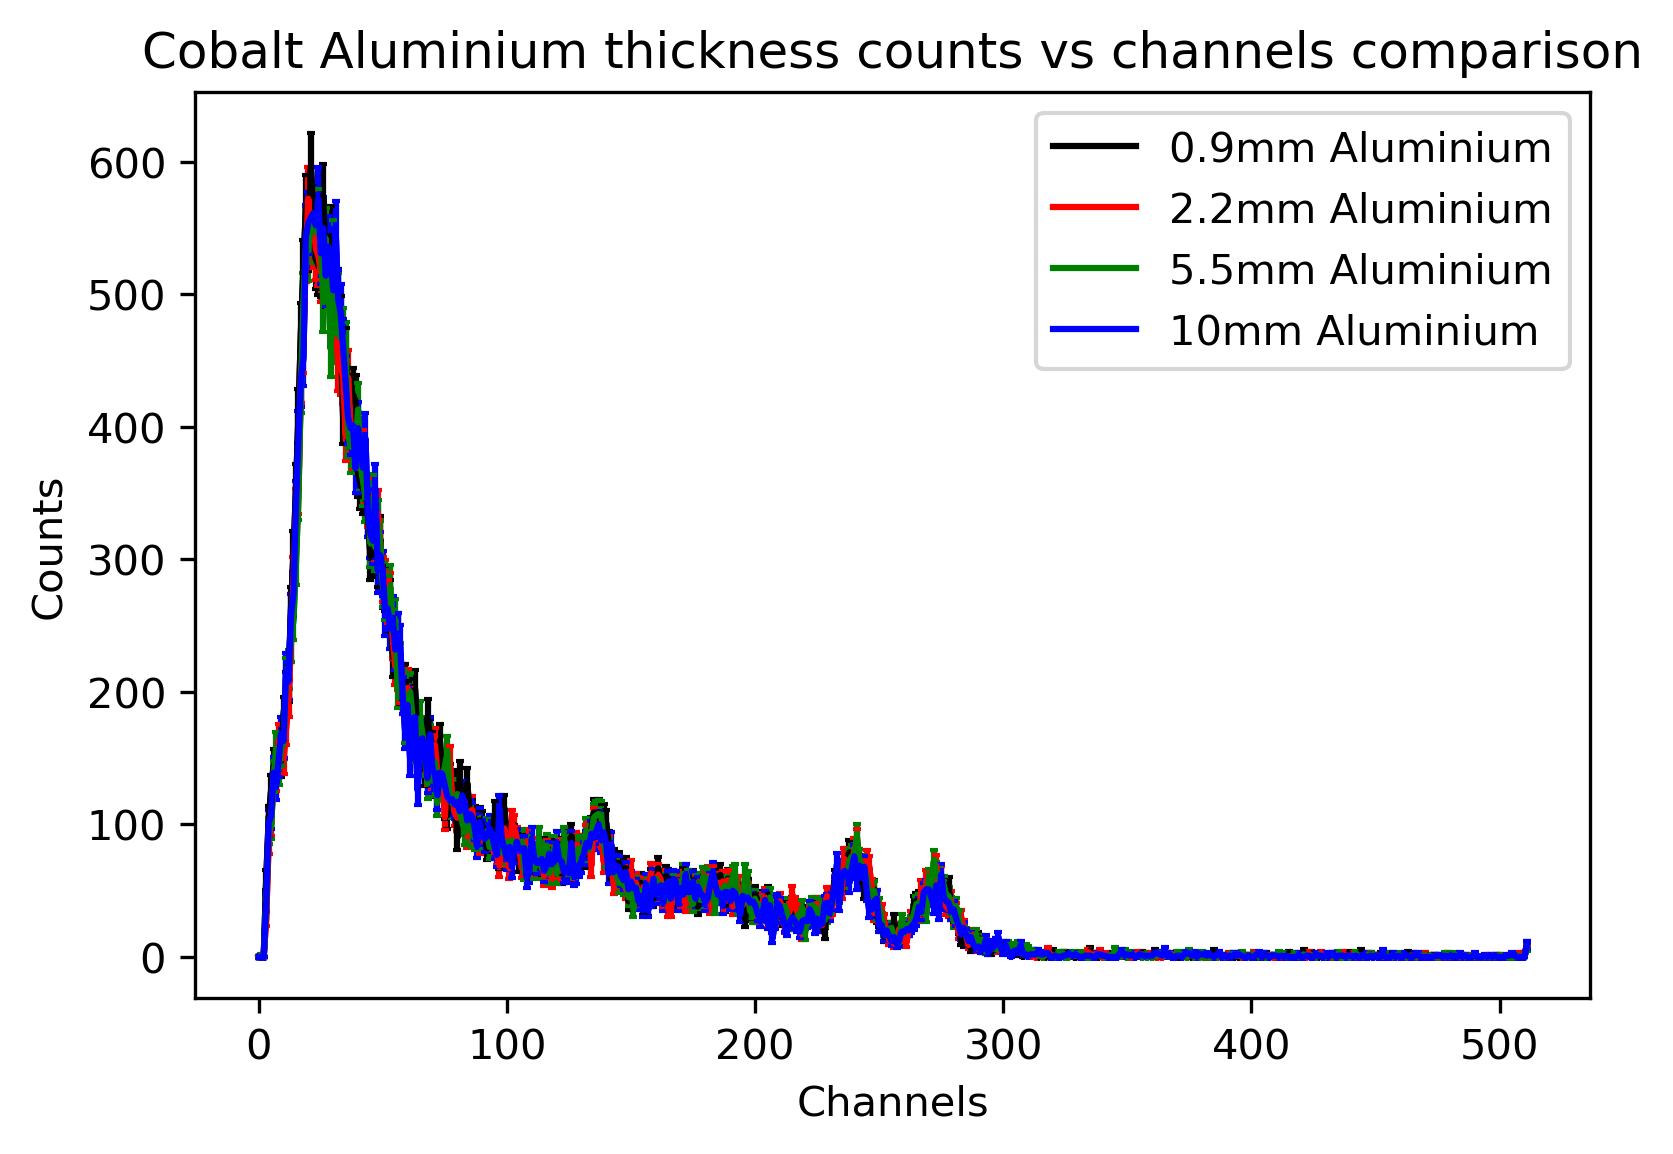
\includegraphics[scale=0.6]{Images/CobaltAluminiumCounts.png}
\caption{Graphical representation of raw data sourced from Cassy showing Aluminium thickness counts of Cobalt.}
\label{Cobalt Alu Counts}
\end{figure}
\end{multicols}
\newpage
\begin{multicols}{2}
\begin{figure}[H]
\centering
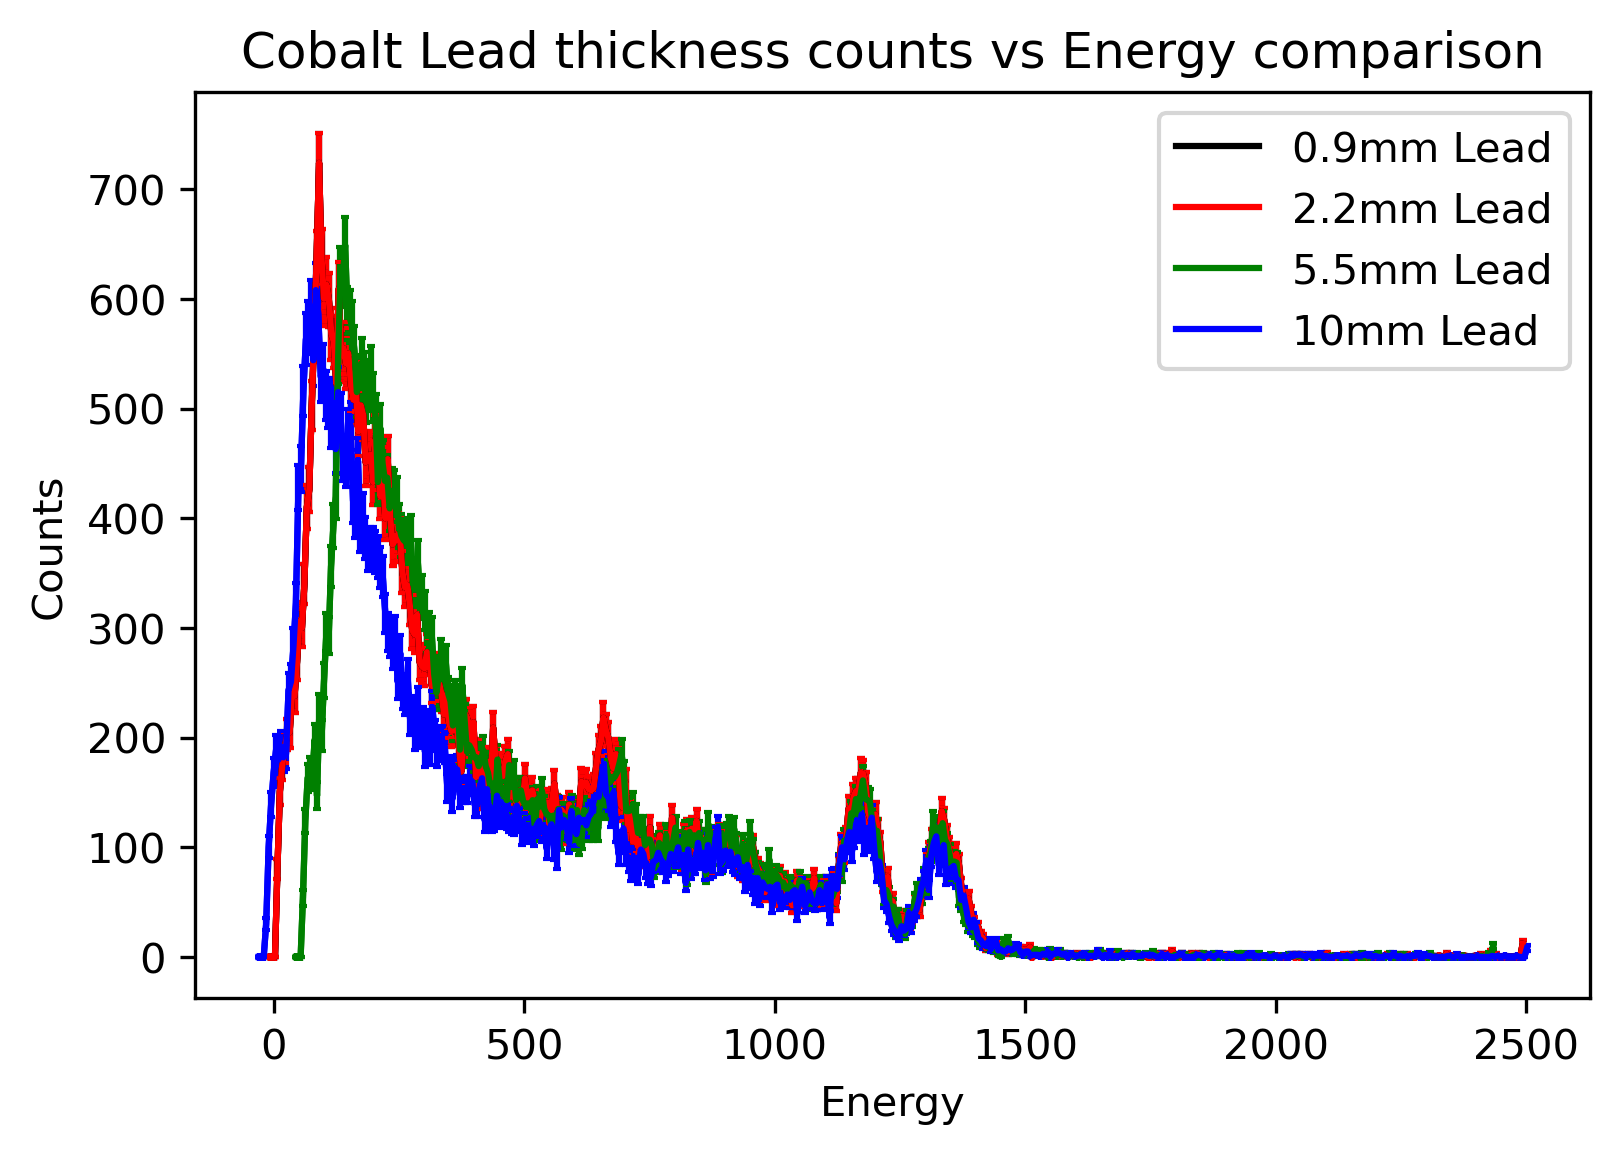
\includegraphics[scale=0.6]{Images/CobaltLeadEnergyCounts.png}
\caption{Graphical representation of raw data sourced from Cassy showing Lead thickness counts vs energy of Cobalt.}
\label{Cobalt Lead Energy Counts}
\end{figure}

\begin{figure}[H]
\centering
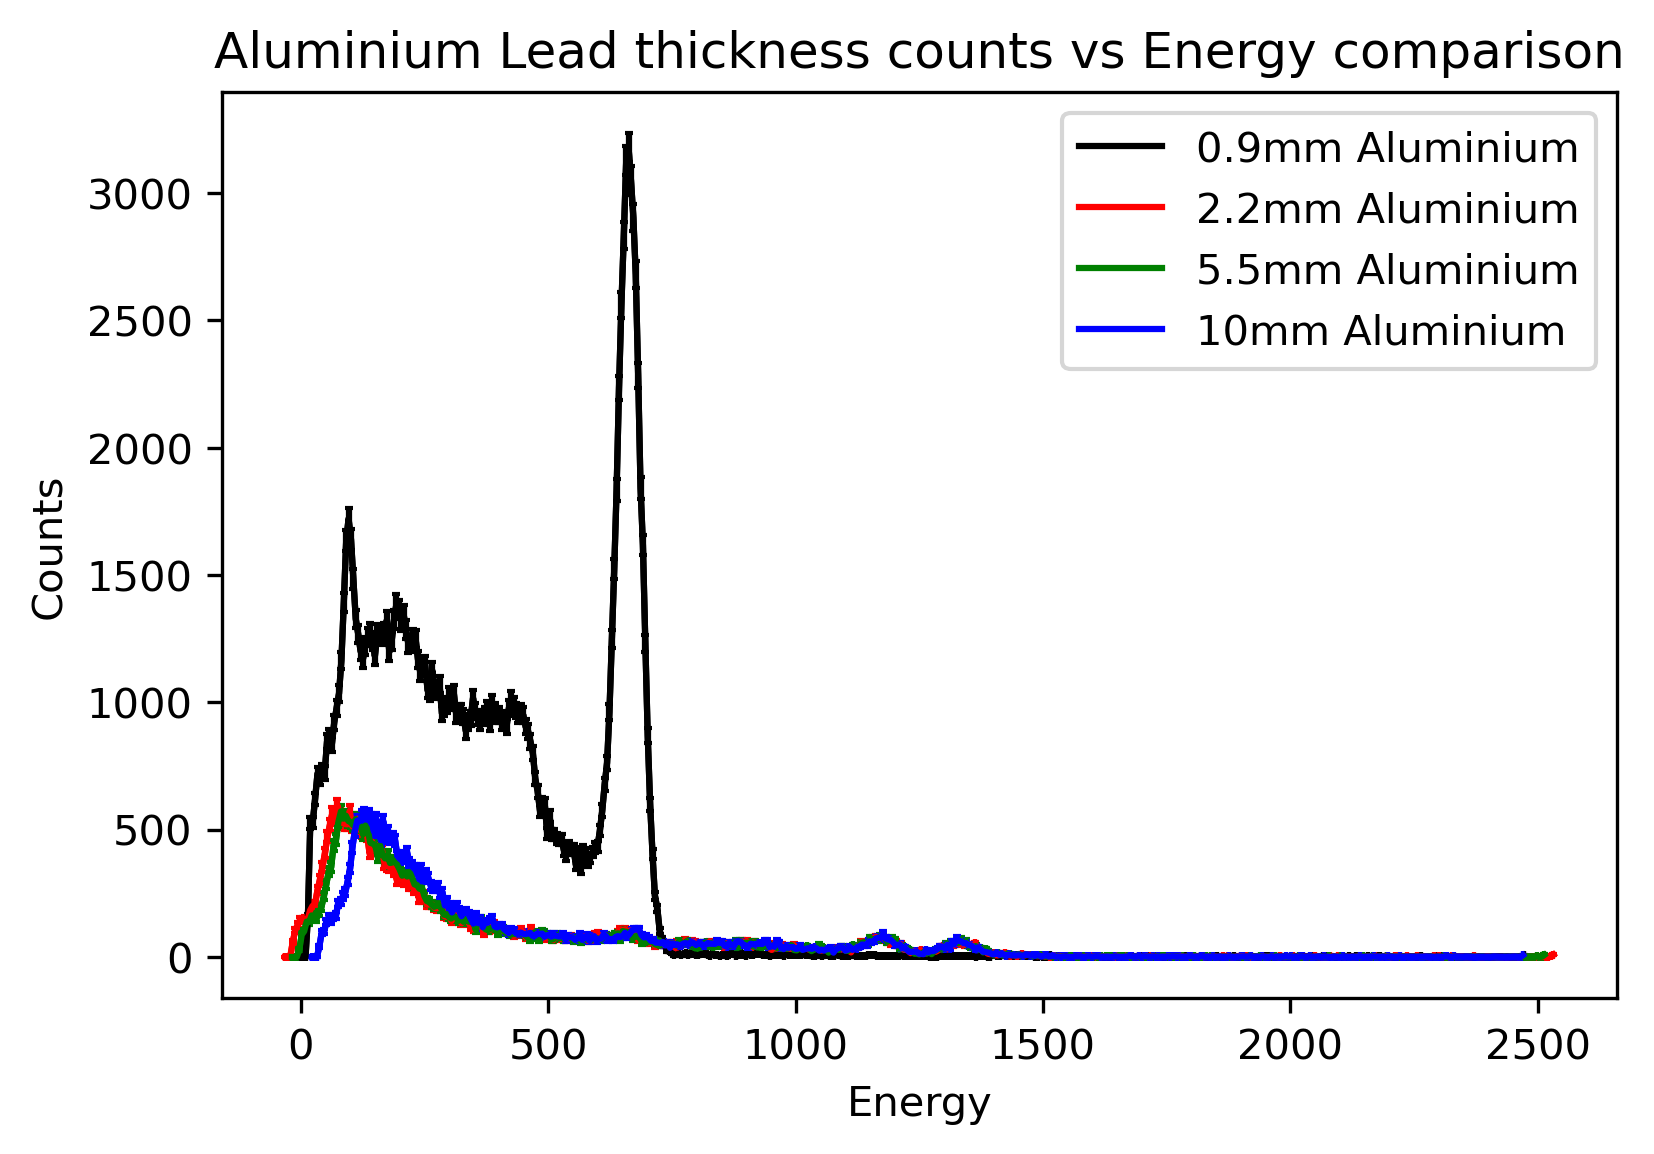
\includegraphics[scale=0.6]{Images/CobaltAluminiumEnergyCounts.png}
\caption{Graphical representation of raw data sourced from Cassy showing Aluminium thickness counts vs energy of Cobalt.}
\label{Cobalt Alu Energy Counts}
\end{figure}
\end{multicols}



\begin{multicols}{2}
\begin{figure}[H]
\centering
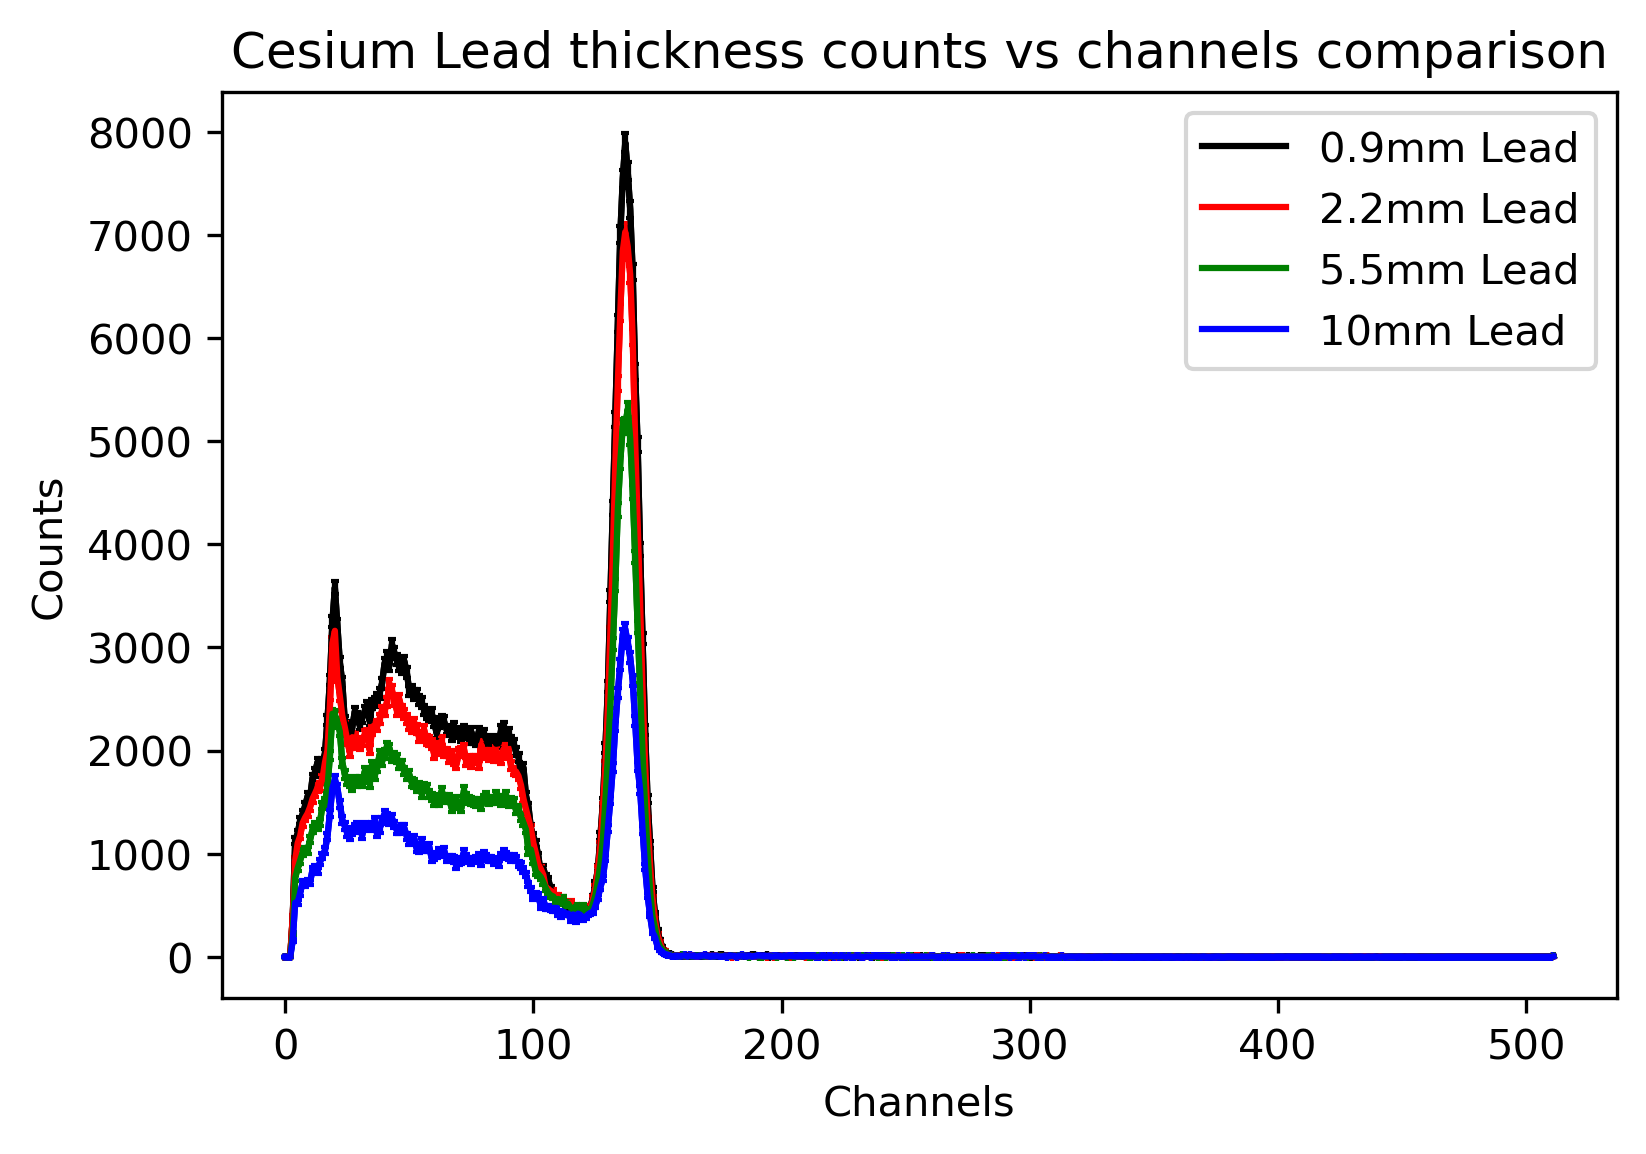
\includegraphics[scale=0.6]{Images/CesiumLeadCounts.png}
\caption{Graphical representation of raw data sourced from Cassy showing Lead thickness counts of Cesium.}
\label{Cesium Lead Counts}
\end{figure}

\begin{figure}[H]
\centering
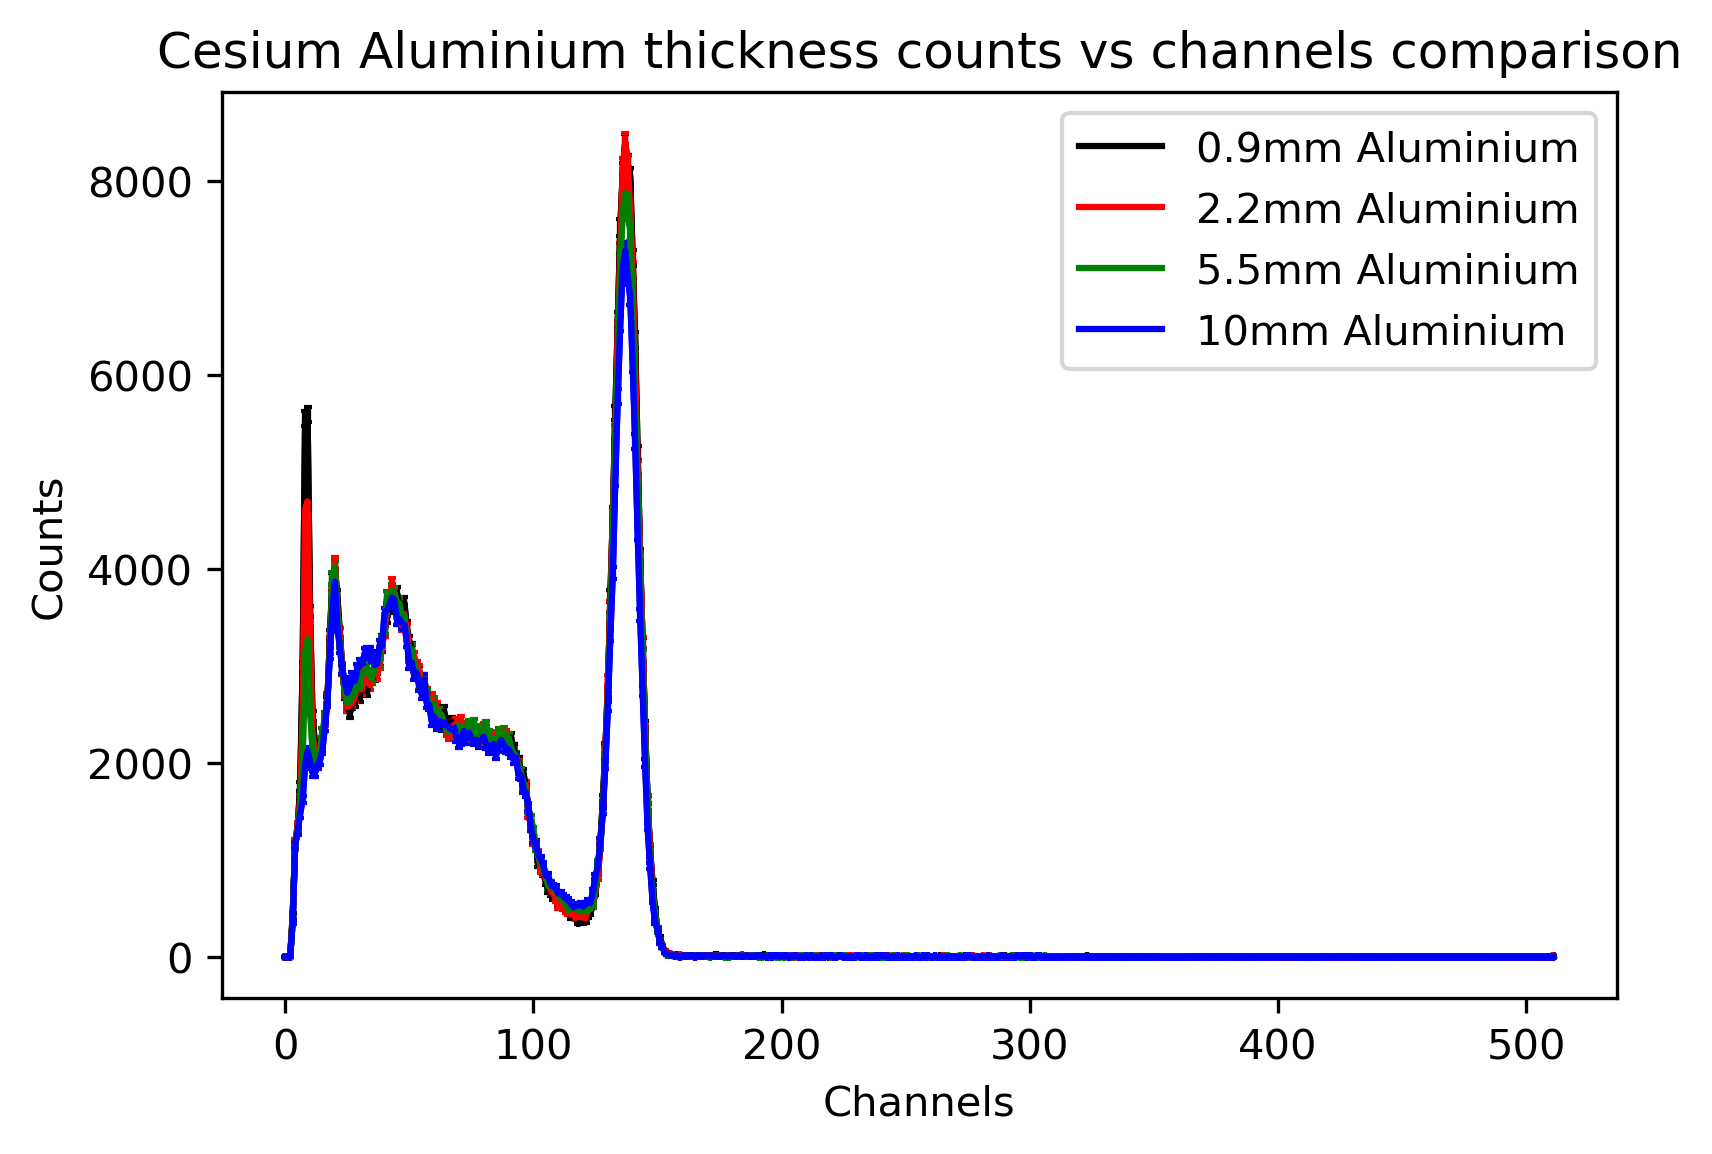
\includegraphics[scale=0.6]{Images/CesiumAluminiumCounts.png}
\caption{Graphical representation of raw data sourced from Cassy showing Aluminium thickness counts of Cesium.}
\label{Cesium Alu Counts}
\end{figure}
\end{multicols}
\newpage
\begin{multicols}{2}
\begin{figure}[H]
\centering
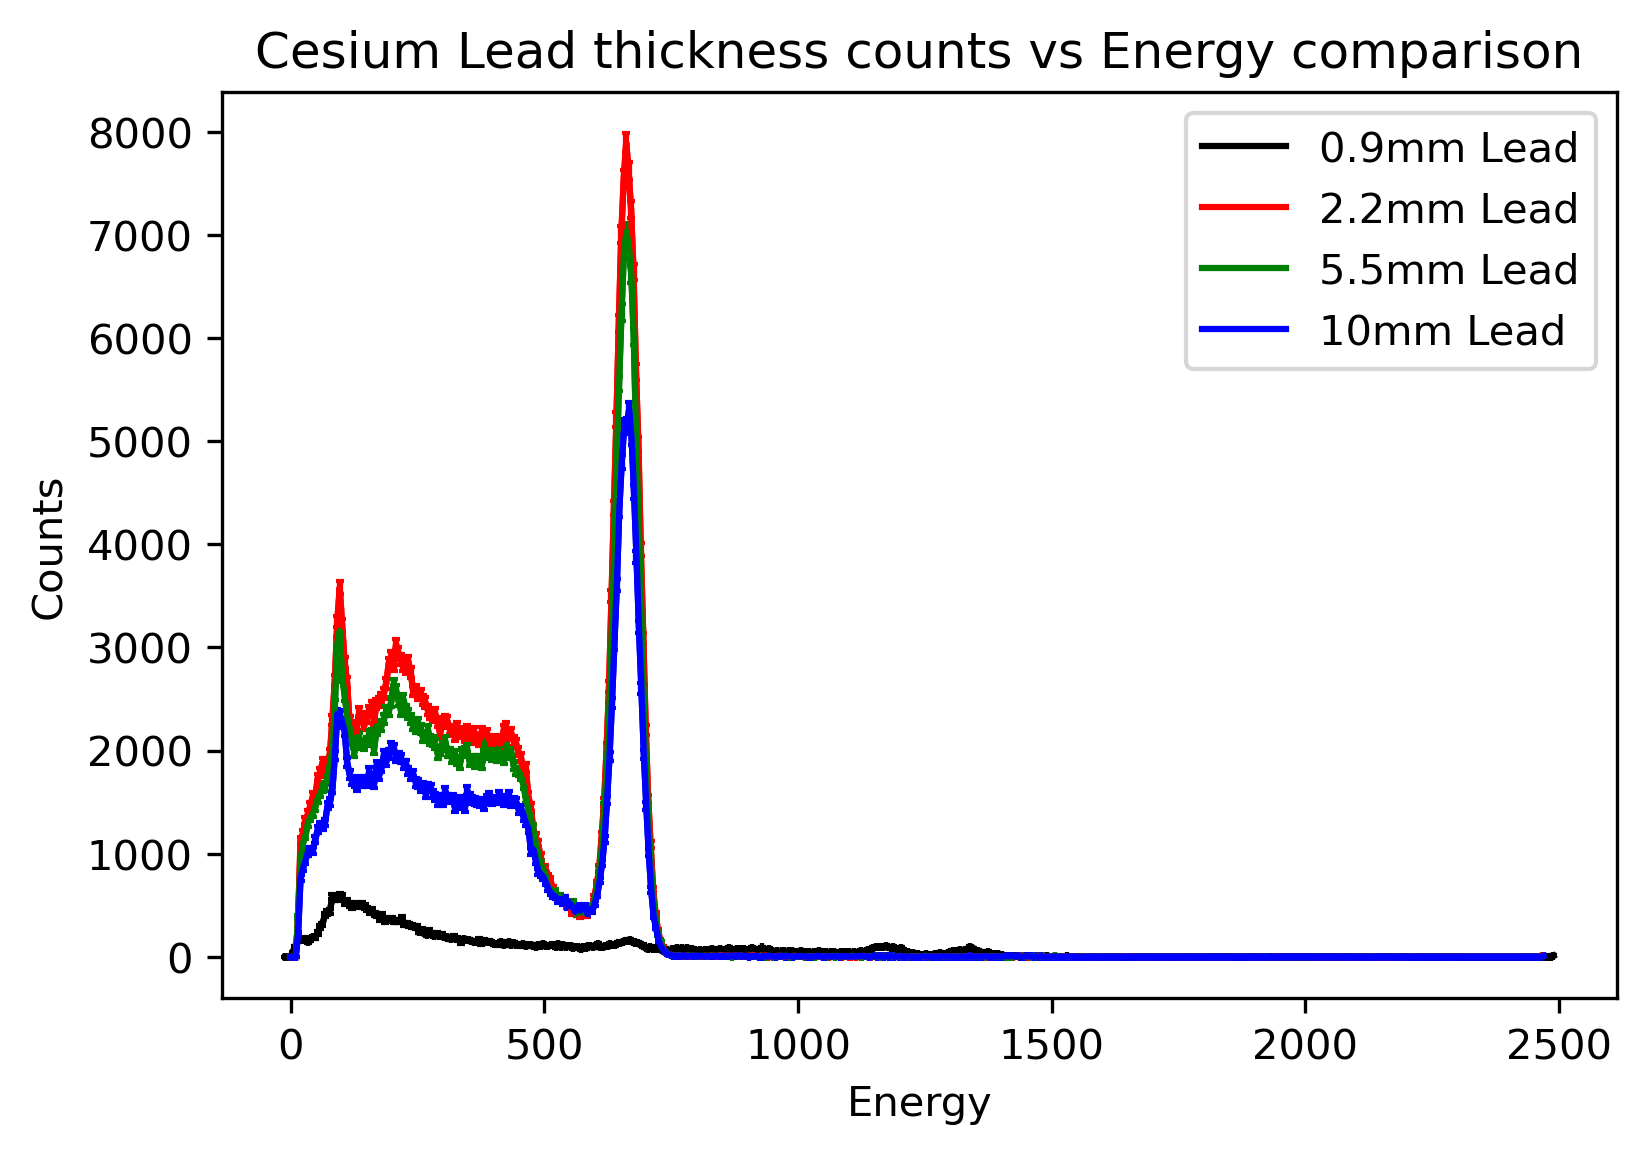
\includegraphics[scale=0.6]{Images/CesiumLeadEnergyCounts.png}
\caption{Graphical representation of raw data sourced from Cassy showing Lead thickness counts vs energy of Cesium.}
\label{Cesium Lead Energy Counts}
\end{figure}

\begin{figure}[H]
\centering
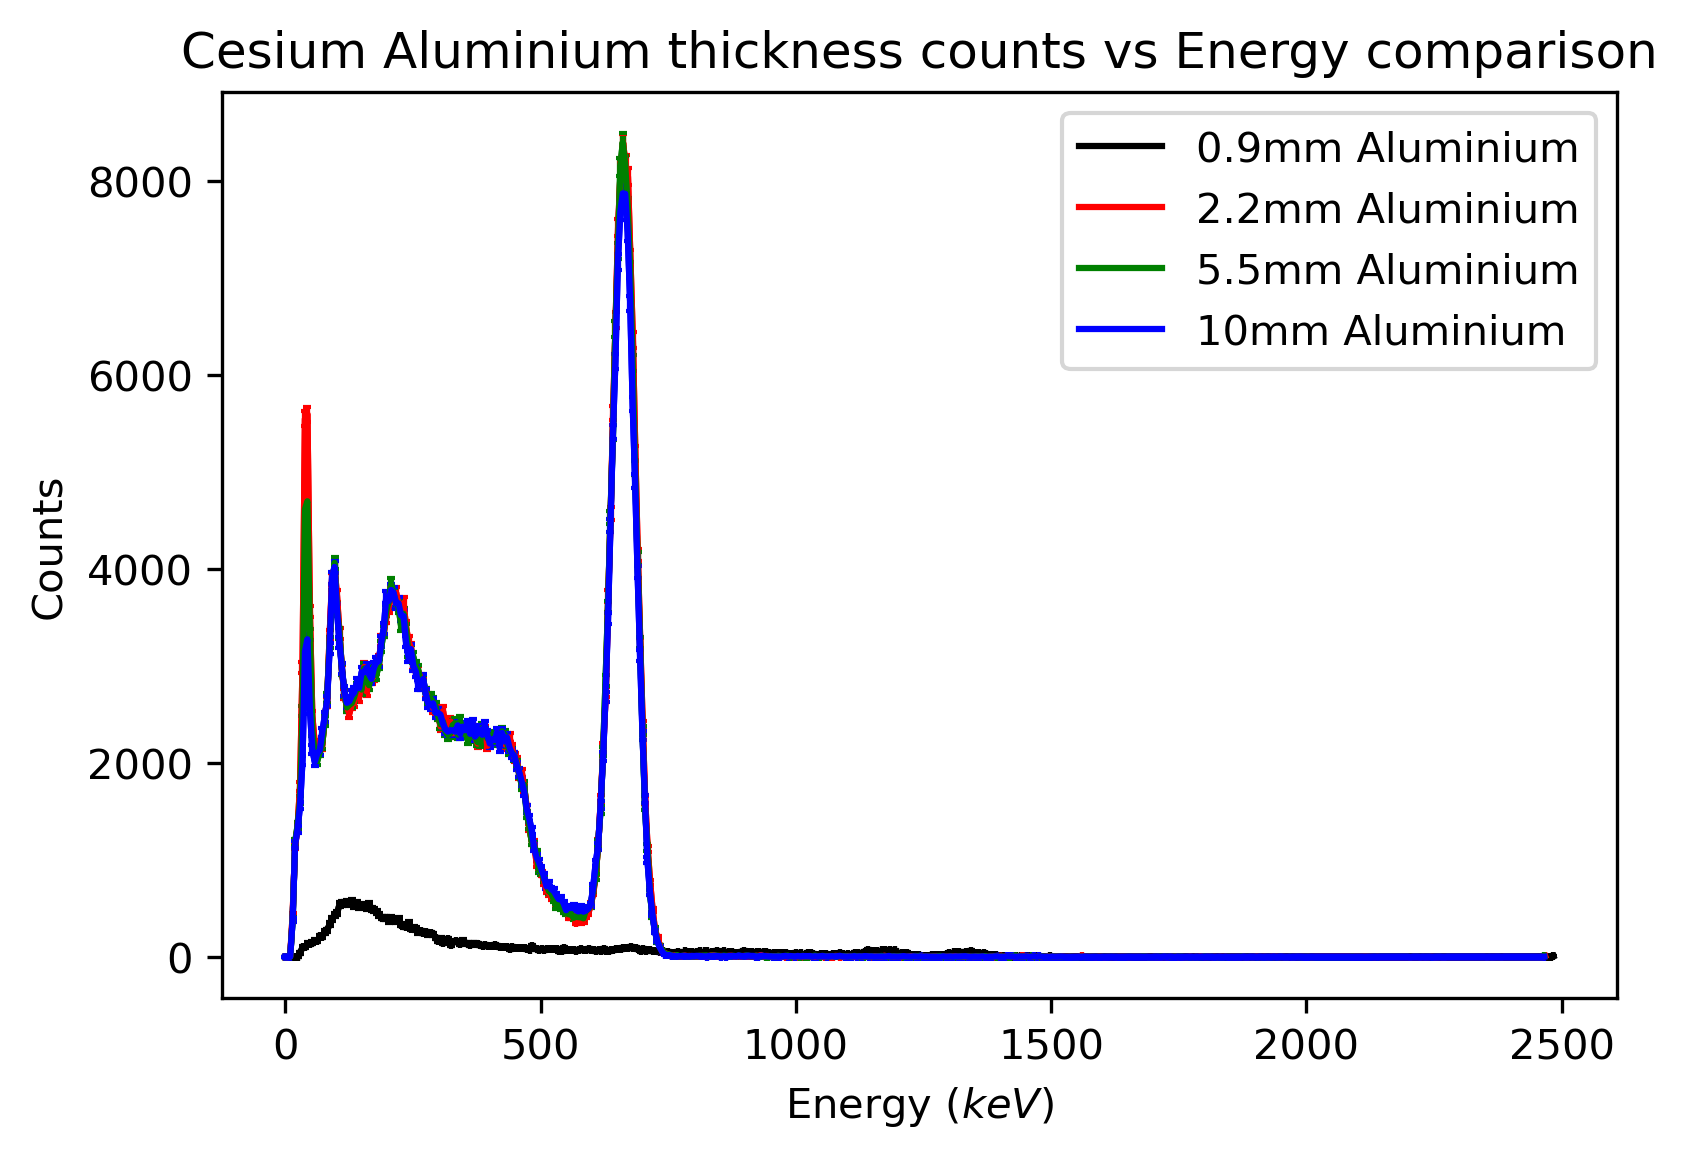
\includegraphics[scale=0.6]{Images/CesiumAluminiumEnergyCounts.png}
\caption{Graphical representation of raw data sourced from Cassy showing Aluminium thickness counts vs energy of Cesium.}
\label{Cesium Alu Energy Counts}
\end{figure}
\end{multicols}

Analysing the above graphs show that as thickness increases the counts also decrease stating that not as many gamma rays and penetrating the material which is to be expected as more atoms are in the way of the travelling gamma rays. Though in Cobalt aluminium counts \cref{Cobalt Alu Counts} it shows very little intensity degradation compared to the Cobalt lead counts \cref{Cobalt Lead Counts} indicating that gamma rays cannot penetrate through thick amounts of lead. The Cesium replicates the statement above when it the gamma ray intensity count is lower in lead than in the aluminium.\\

\begin{table}[H]
\begin{center}
 \footnotesize
 \begin{tabular}{|c||c||c|c|c|c||c|c|c|c|}
 \hline
 \multicolumn{10}{|c|}{Table of data for different material thicknesses against Cobalt} \\
 \hline \hline
 \multicolumn{1}{|c||}{} & \multicolumn{1}{|c||}{$^{60}Cobalt$} & \multicolumn{4}{|c||}{Lead} & \multicolumn{4}{c|}{Aluminium} \\
 \hline
  Energy & Thickness & 0.0009m & 0.0022m & 0.0055m & 0.017m & 0.0009m & 0.0022m & 0.0055m & 0.017m\\
 \hline \hline
  (MeV)& Compton Count & 87482 & 87016 &76745 & 72851 & 94683 & 92657 & 90142 & 84850 \\
 \hline \hline
 1.17 Mev & Peak Count & 241.3 & 241.2 & 242.9 & 242.0 & 240.1 & 240.4 & 240.1 & 239.7 \\
 \hline
 1.17 Mev & Peak Count $\sigma$ & $\pm$3.1 & $\pm$4.3 & $\pm$4.1 & $\pm$3.7 & $\pm$5.2 & $\pm$5.8 & $\pm$5.3 & $\pm$5.4 \\
 \hline
 1.17 Mev & Peak Integral & 1063 & 942 & 935 & 897 & 1450 & 1387 & 1356 & 1348 \\
 \hline
 1.17 Mev & Energy (keV) & 1170.84 & 1171.13 & 1170.90 & 1171.74 & 1170.48 & 1172.96 & 1172.61 & 1170.73 \\
 \hline
 1.17 Mev & Energy $\sigma$ (keV) & $\pm$14.35 & $\pm$14.90 & $\pm$15.82 & $\pm$14.71 & $\pm$27.19 & $\pm$28.88 & $\pm$24.76 & $\pm$27.10 \\
 \hline \hline
 1.33 Mev & Peak Count & 273.8 & 275.4 & 275.0 & 274.5 & 272.2 & 272.5 & 273.3 & 273.6 \\
 \hline
 1.33 Mev & Peak Count $\sigma$ & $\pm$4.0 & $\pm$4.2 & $\pm$4.4 & $\pm$2.7 & $\pm$5.1 & $\pm$5.2 & $\pm$4.6 & $\pm$6.3 \\
 \hline
 1.33 Mev & Peak Integral & 963 & 912 & 901 & 894 & 1035 & 1028 & 1014 & 932 \\
 \hline
 1.33 Mev & Energy (keV) & 1328.96 & 1330.55 & 1329.59 & 1331.84 & 1334.04 & 1331.78 & 1327.30 & 1333.05 \\
 \hline
 1.33 Mev & Energy $\sigma$ (keV) & $\pm$12.7 & $\pm$14.3 & $\pm$13.7 & $\pm$13.2 & $\pm$27.2 & $\pm$26.2 & $\pm$21.8 & $\pm$29.5 \\
 \hline
 \end{tabular} \\ 
 \caption{Table of data for different material thicknesses against Cobalt}
 \label{Cobalt Data}
\end{center}
\end{table} 

\begin{table}[H]
\begin{center}
 \footnotesize
 \begin{tabular}{|c||c||c|c|c|c||c|c|c|c|}
 \hline
 \multicolumn{10}{|c|}{Table of data for different material thicknesses against Cesium} \\
 \hline \hline
 \multicolumn{1}{|c||}{} & \multicolumn{1}{|c||}{$^{137}Cesium$} & \multicolumn{4}{|c||}{Lead} & \multicolumn{4}{c|}{Aluminium} \\
 \hline
  Energy & Thickness & 0.0009m & 0.0022m & 0.0055m & 0.017m & 0.0009m & 0.0022m & 0.0055m & 0.017m\\
 \hline \hline
  (MeV) & Compton Count & 189,472 & 1118,483 & 114,820 & 109,907 & 271,476 & 266,016 & 263,875 & 257,334 \\
 \hline \hline
 0.66 & Peak Count & 137.1 & 137.0 & 136.9 & 136.8 & 137.0 & 137.1 & 137.1 & 137.0 \\
 \hline
 0.66 & Peak Count $\sigma$ & $\pm$4.6 & $\pm$4.4 & $\pm$4.3 & $\pm$4.2 & $\pm$4.5 & $\pm$4.4 & $\pm$4.4 & $\pm$4.3 \\
 \hline
 0.66 & Peak Integral & 98,622 & 86,728 & 66,829 & 40,956 & 103912 & 101986 & 98697 & 90533 \\
 \hline
 0.66 & Energy (keV) & 661.66 & 661.82 & 661.84 & 661.53 & 662.07 & 661.46 & 661.81 & 661.33 \\
 \hline
 0.66 & Energy $\sigma$ (keV) & $\pm$22.35 & $\pm$21.31 & $\pm$20.93 & $\pm$20.36 & $\pm$21.43 & $\pm$21.66 & $\pm$21.18 & $\pm$20.92 \\
 \hline
 \end{tabular} \\ 
 \caption{Table of data for different material thicknesses against Cesium}
 \label{Cobalt Data}
\end{center}
\end{table}

Though as stated earlier the gamma rays interfere with the materials atoms as they pass through getting absorbed or destroyed and as both the materials lead and aluminium have different densities and atomic structure, this must be taken into account by determining the linear and mass attenuation co-efficient.

%---------------------------------------------------------------------------
\subsubsection{Linear Attenuation Co-efficient}
\label{LAC SubsubSection}

The linear attenuation co-efficient is calculated by\cite{Exp.C-2020}:

\begin{equation}
I = I_0 e^{-\mu*x} 
\label{I1 Eq}
\end{equation}

\begin{equation}
In(I) = In(I_0) + In(e^{-\mu*x})
\label{I2 Eq}
\end{equation} 

\begin{equation}
In(I) = In(I_0) -\mu*x \xrightarrow{} -\mu*x + In(I_0)
\label{I3 Eq}
\end{equation} 

\begin{equation}
In(I) = -\mu*x + In(I_0) \xrightarrow{} y=mx+c
\label{I4 Eq}
\end{equation} 

By changing the linear attenuation co-efficient equation into a linear scale instead of a log scale, the similarities between the L.A.C. equation and straight line equation of y=mx+c. As shown in \cref{LACgraph} the linear attenuation co-efficient $\mu$ is negative in the equation, the simplified assumption is that this negative sign is ignored as the value of m is the target that displays as the linear attenuation co-efficient. These gradient values are sourced as a values of m and turned positive to to display as the linear attenuation co-efficient. \\

\begin{figure}[H]
\centering
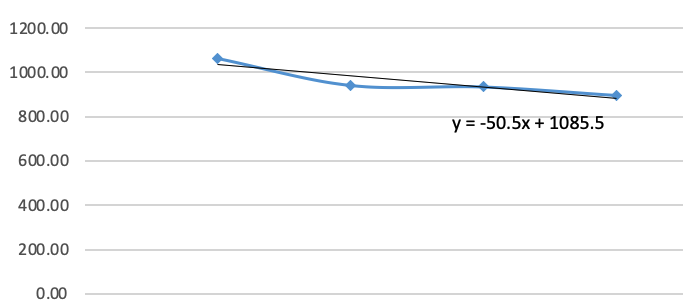
\includegraphics[scale=0.6]{Images/LAC.png}
\caption{Gradient of absorption data that translates into the linear attenuation coefficient.}
\label{LACgraph}
\end{figure}

\begin{table}[H]
\begin{center}
 \footnotesize
 \begin{tabular}{|c||c|c|c|c||c|c|}
 \hline
 \multicolumn{1}{|c||}{L.A.C} & \multicolumn{4}{|c||}{Cobalt} & \multicolumn{2}{c|}{Cesium} \\
 \hline
  DATA & 1.17 MeV & 1.17 MeV $\sigma$ & 1.33 MeV & 1.33 MeV $\sigma$ & 0.66 MeV & 0.66 MeV $\sigma$\\
 \hline \hline
  Lead & 50.5 & $\pm$0.0875 & 21.8 & $\pm$0.358 & 19398 & $\pm$37.365 \\
 \hline \hline
  Aluminium & 33.7 & $\pm$0.451 & 32.8 & $\pm$0.514 & 4342 & $\pm$6.9592 \\
 \hline
 \end{tabular} \\ 
 \caption{L.A.C. data collected from \cref{I4 Eq}}
 \label{LAC Data}
\end{center}
\end{table}

%---------------------------------------------------------------------------
\subsubsection{Mass Attenuation Co-efficient}
\label{MAC SubsubSection}

As the linear attenuation co-efficient for each material and energy peak is calculated the mass attenuation co-efficient is then calculated taking into account a difference between the materials lead and aluminium which is their densities. The linear attenuation co-efficient $\mu$ is taken from \cref{LAC Data} and taking the density $\rho$ for lead as 11340$kg/m^3$ and for aluminium is 2700$kg/m^3$ where these values are plugged into \cref{MAC Eq} and outputted in \cref{MAC Data}.

\begin{equation}
\mu_m = \dfrac{\mu}{\rho}
\label{MAC Eq}
\end{equation} 

\begin{table}[H]
\begin{center}
 \footnotesize
 \begin{tabular}{|c||c|c|c|c||c|c|}
 \hline
 \multicolumn{1}{|c||}{M.A.C} & \multicolumn{4}{|c||}{Cobalt} & \multicolumn{2}{c|}{Cesium} \\
 \hline
  DATA & 1.17 MeV & 1.17 MeV $\sigma$ & 1.33 MeV & 1.33 MeV $\sigma$ & 0.66 MeV & 0.66 MeV $\sigma$\\
 \hline \hline
  Lead & 0.00445 & $\pm$0.00007 & 0.00192 & $\pm$0.0003 & 1.71058 & $\pm$0.00329 \\
 \hline
 Aluminium & 0.01248 & $\pm$0.000017 & 0.01196 & $\pm$0.00019 & 1.60815 & $\pm$0.00258 \\
 \hline
 \end{tabular} \\ 
 \caption{}
 \label{MAC Data}
\end{center}
\end{table}
 
%---------------------------------------------------------------------------
\subsubsection{Corrected Results}
\label{Corrected Results SubsubSection}

Using \cref{I4 Eq} the values of data sourced in \cref{Absorption SubSection} is recalculated and tabulated in \cref{Corrected Data} displayed graphically below. 
 
\begin{table}[H]
\begin{center}
 \footnotesize
 \begin{tabular}{|c||c|c|c|c|}
 \hline
 $^{60}Cobalt$ Lead & 0.0009m & 00022m & 0.0055m & 0.017m \\
 \hline
 1.17 MeV Intensity & 3.07 & 3.09 & 3.25 & 3.81 \\
 \hline
 1.17 MeV Intensity $\sigma$ & 0.51 & 0.49 & 0.49 & 0.49 \\
 \hline
 1.33 MeV Intensity & 3.00 & 3.01 & 3.07 & 3.32 \\
 \hline
 1.33 MeV Intensity $\sigma$ & 0.49 & 0.48 & 0.48 & 0.48 \\
 \hline \hline
  $^{60}Cobalt$ Alu & 0.0009m & 00022m & 0.0055m & 0.017m \\
 \hline
 1.17 MeV Intensity & 3.19 & 3.22 & 3.32 & 3.70 \\
 \hline
 1.17 MeV Intensity $\sigma$ & 0.58 & 0.57 & 0.57 & 0.57 \\
 \hline
 1.33 MeV Intensity & 3.04 & 3.08 & 3.18 & 3.52 \\
 \hline
 1.33 MeV Intensity $\sigma$ & 0.51 & 0.51 & 0.51 & 0.49 \\
 \hline \hline
  $^{137}Cesium$ Lead & 0.0009m & 00022m & 0.0055m & 0.017m \\
 \hline
 0.66 MeV Intensity & 22.45 & 47.61 & 111.51 & 334.37 \\
 \hline
 0.66 MeV Intensity $\sigma$ & 2.53 & 2.55 & 2.62 & 2.94 \\
 \hline \hline
 $^{137}Cesium$ Alu & 0.0009m & 00022m & 0.0055m & 0.017m \\
 \hline
 0.66 MeV Intensity & 8.92 & 14.56 & 28.88 & 78.77 \\
 \hline
 0.66 MeV Intensity $\sigma$ & 2.51 & 2.52 & 2.54 & 2.60 \\
 \hline
 \end{tabular} \\ 
 \caption{Tabulated data of the corrected values of \cref{Absorption SubSection}}
 \label{Corrected Data}
\end{center}
\end{table}

\begin{multicols}{2}
\begin{figure}[H]
\centering
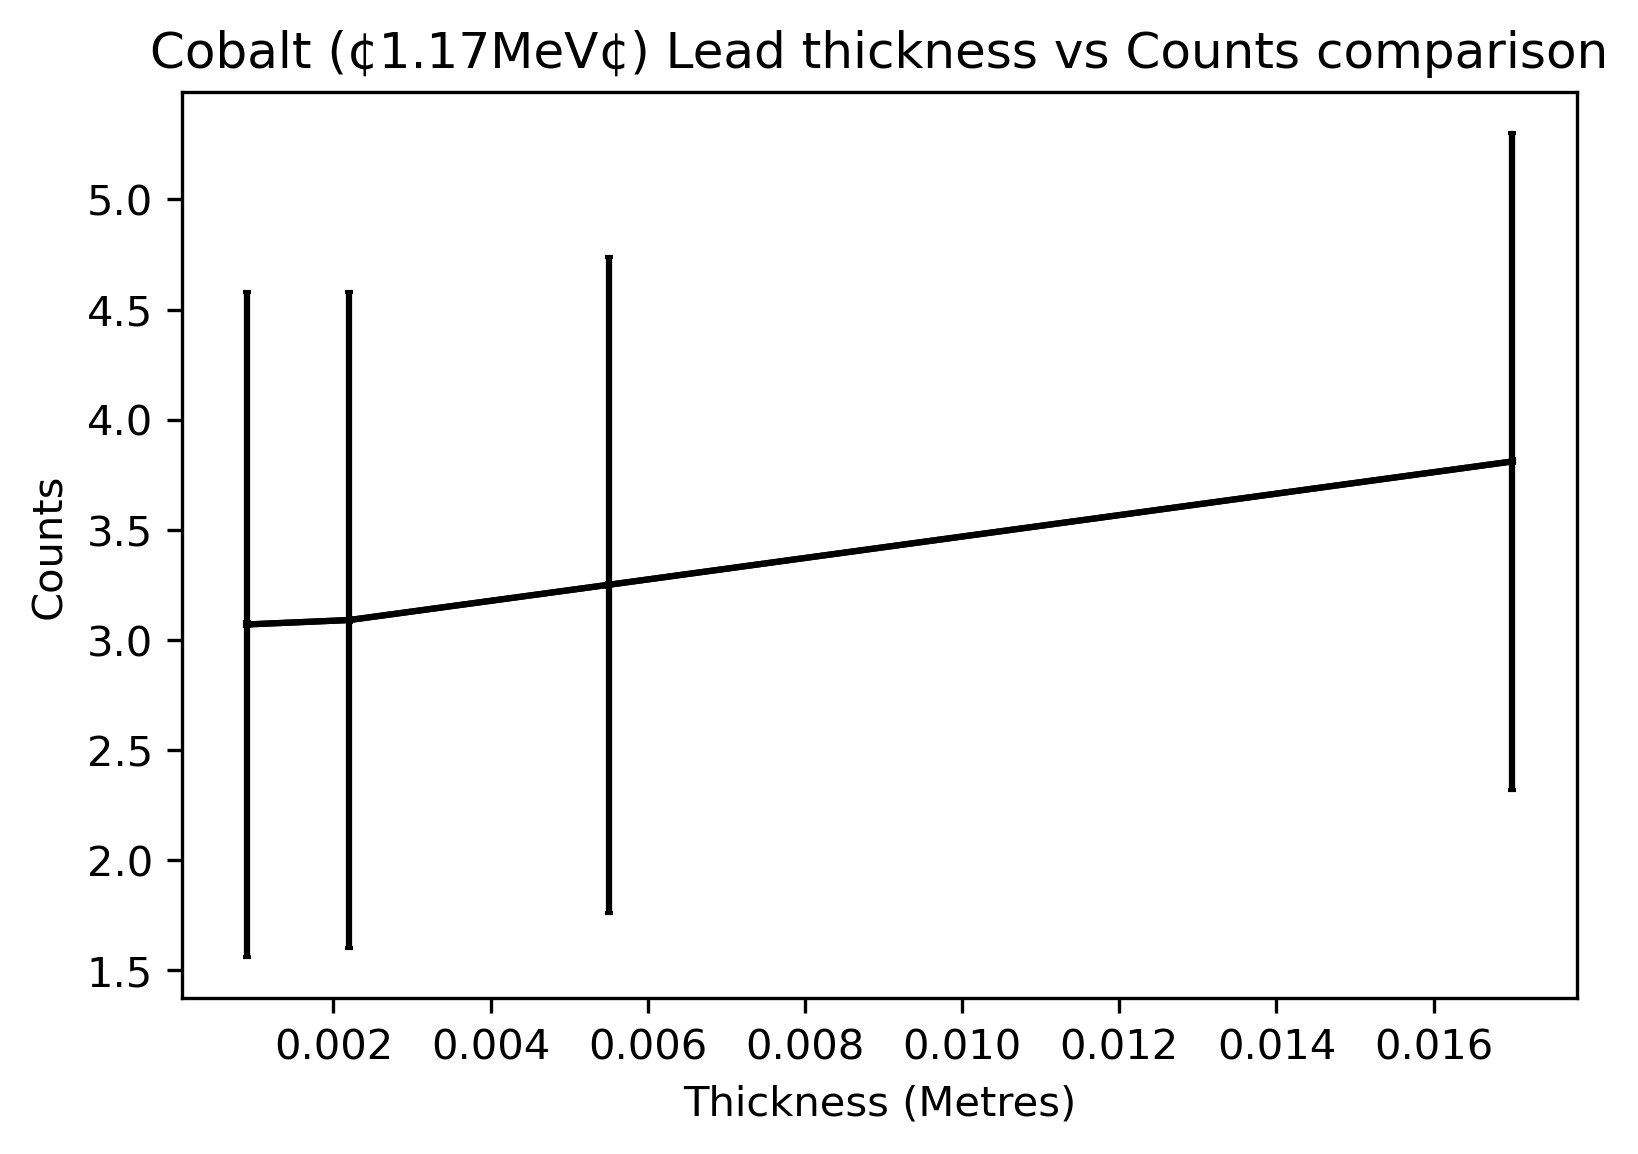
\includegraphics[scale=0.6]{Images/CobaltLead117Final.png}
\caption{Graphical representation of \cref{Corrected Data} for Lead thickness in Cobalt (1.17 MeV).}
\label{Cobalt 117 Lead Final Counts}
\end{figure}

\begin{figure}[H]
\centering
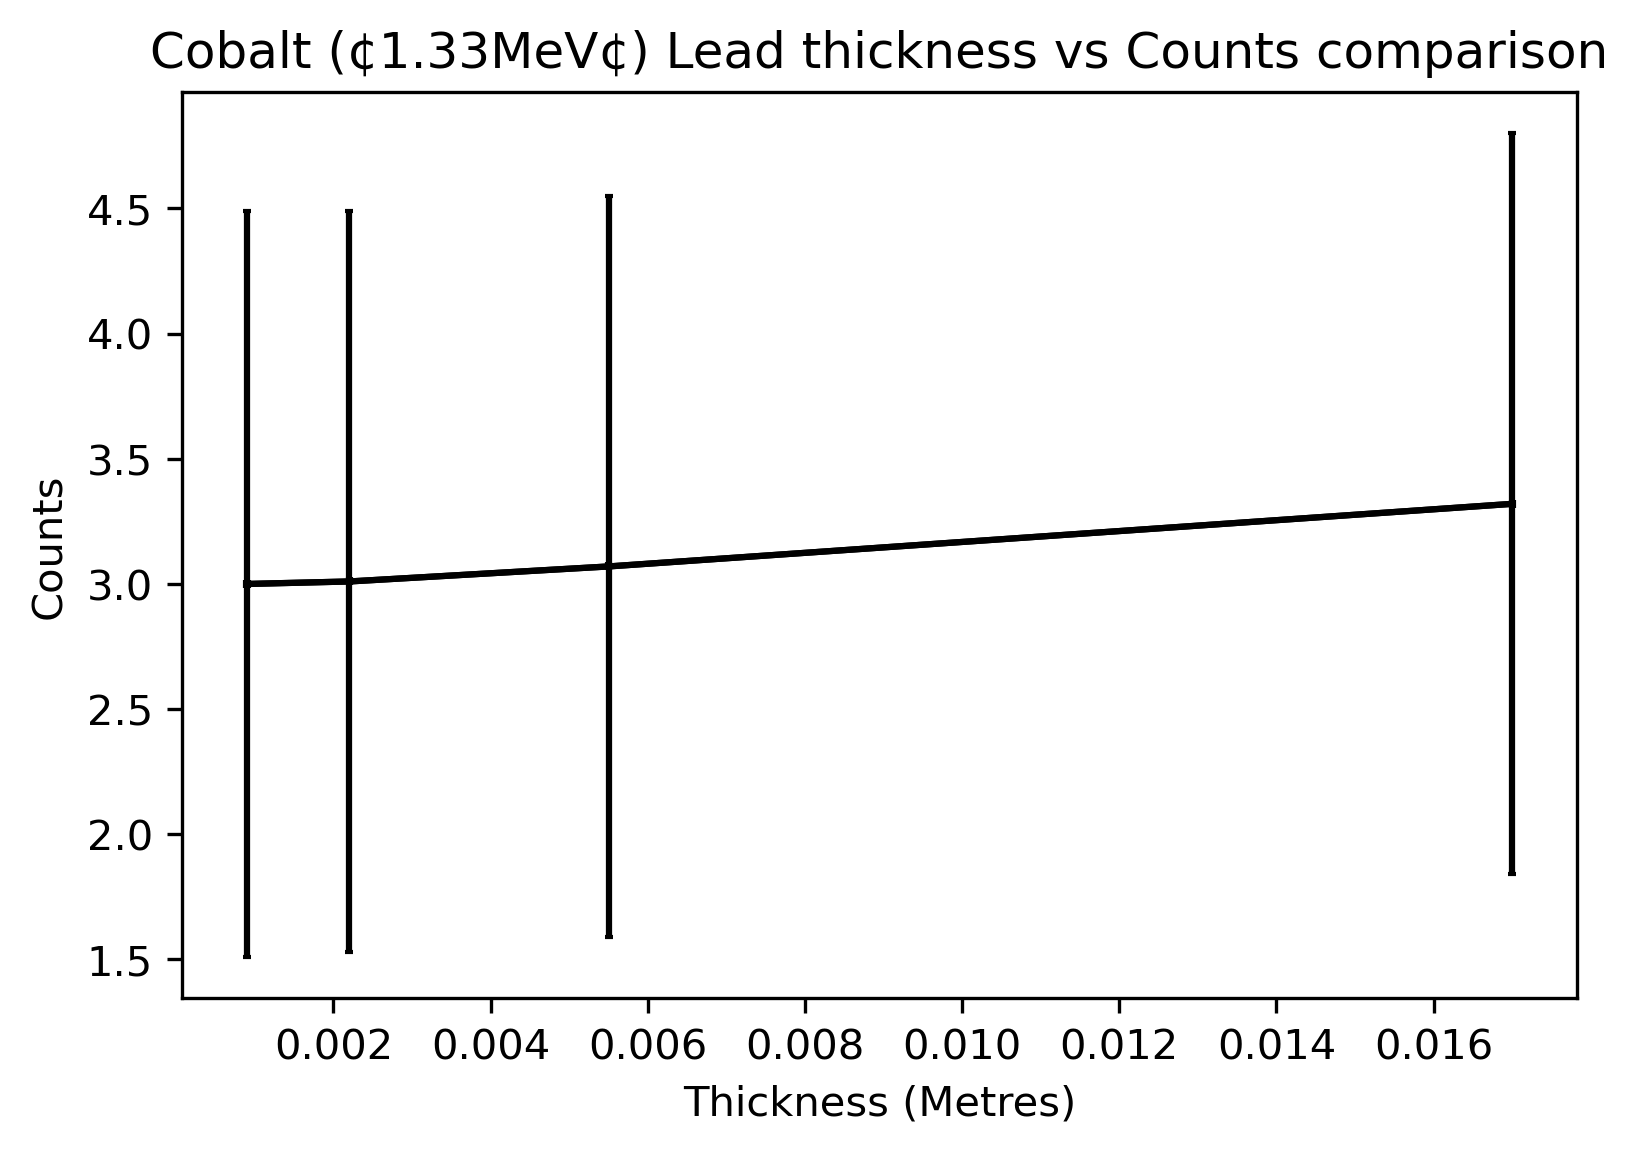
\includegraphics[scale=0.6]{Images/CobaltLead133Final.png}
\caption{Graphical representation of \cref{Corrected Data} for Lead thickness in Cobalt (1.33 MeV).}
\label{Cobalt 133 Lead Final Counts}
\end{figure}
\end{multicols}
\newpage
\begin{multicols}{2}
\begin{figure}[H]
\centering
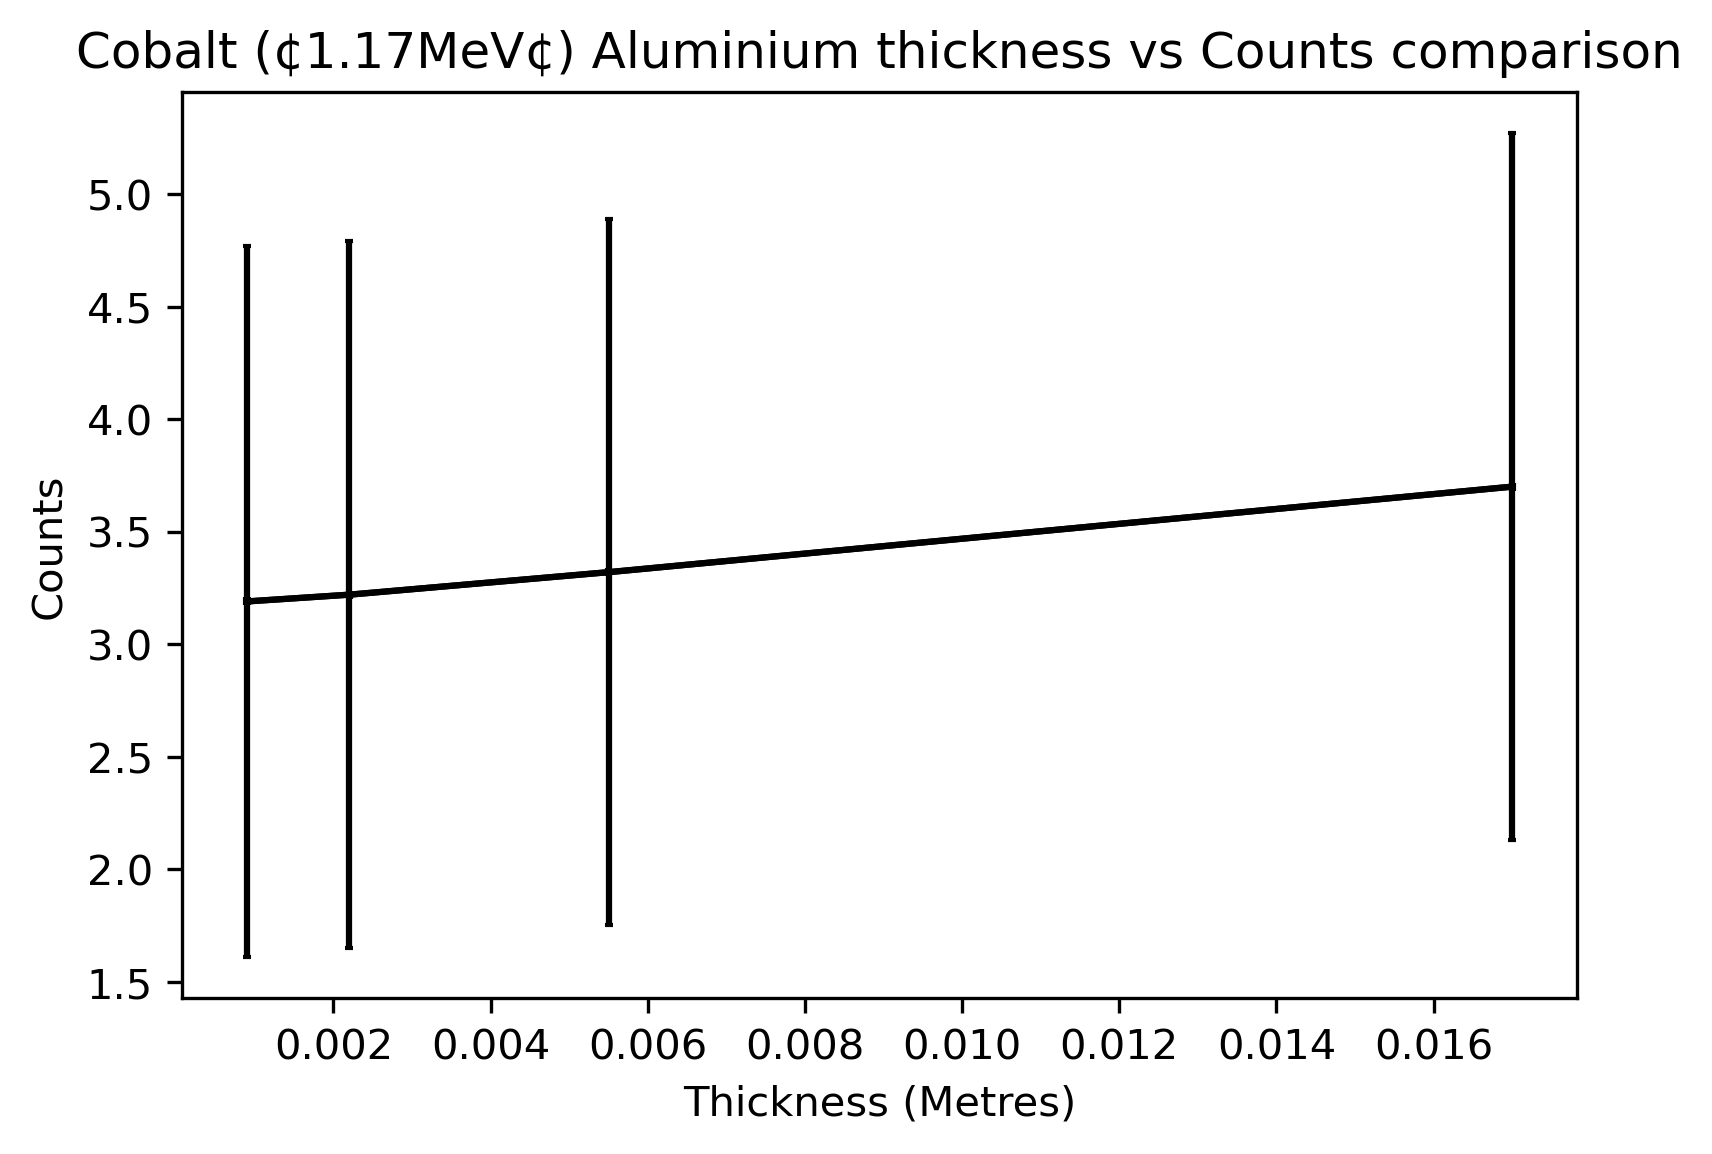
\includegraphics[scale=0.6]{Images/CobaltAlu117Final.png}
\caption{Graphical representation of \cref{Corrected Data} for Aluminium thickness in Cobalt (1.17 MeV).}
\label{Cobalt 117 Alu Final Counts}
\end{figure}

\begin{figure}[H]
\centering
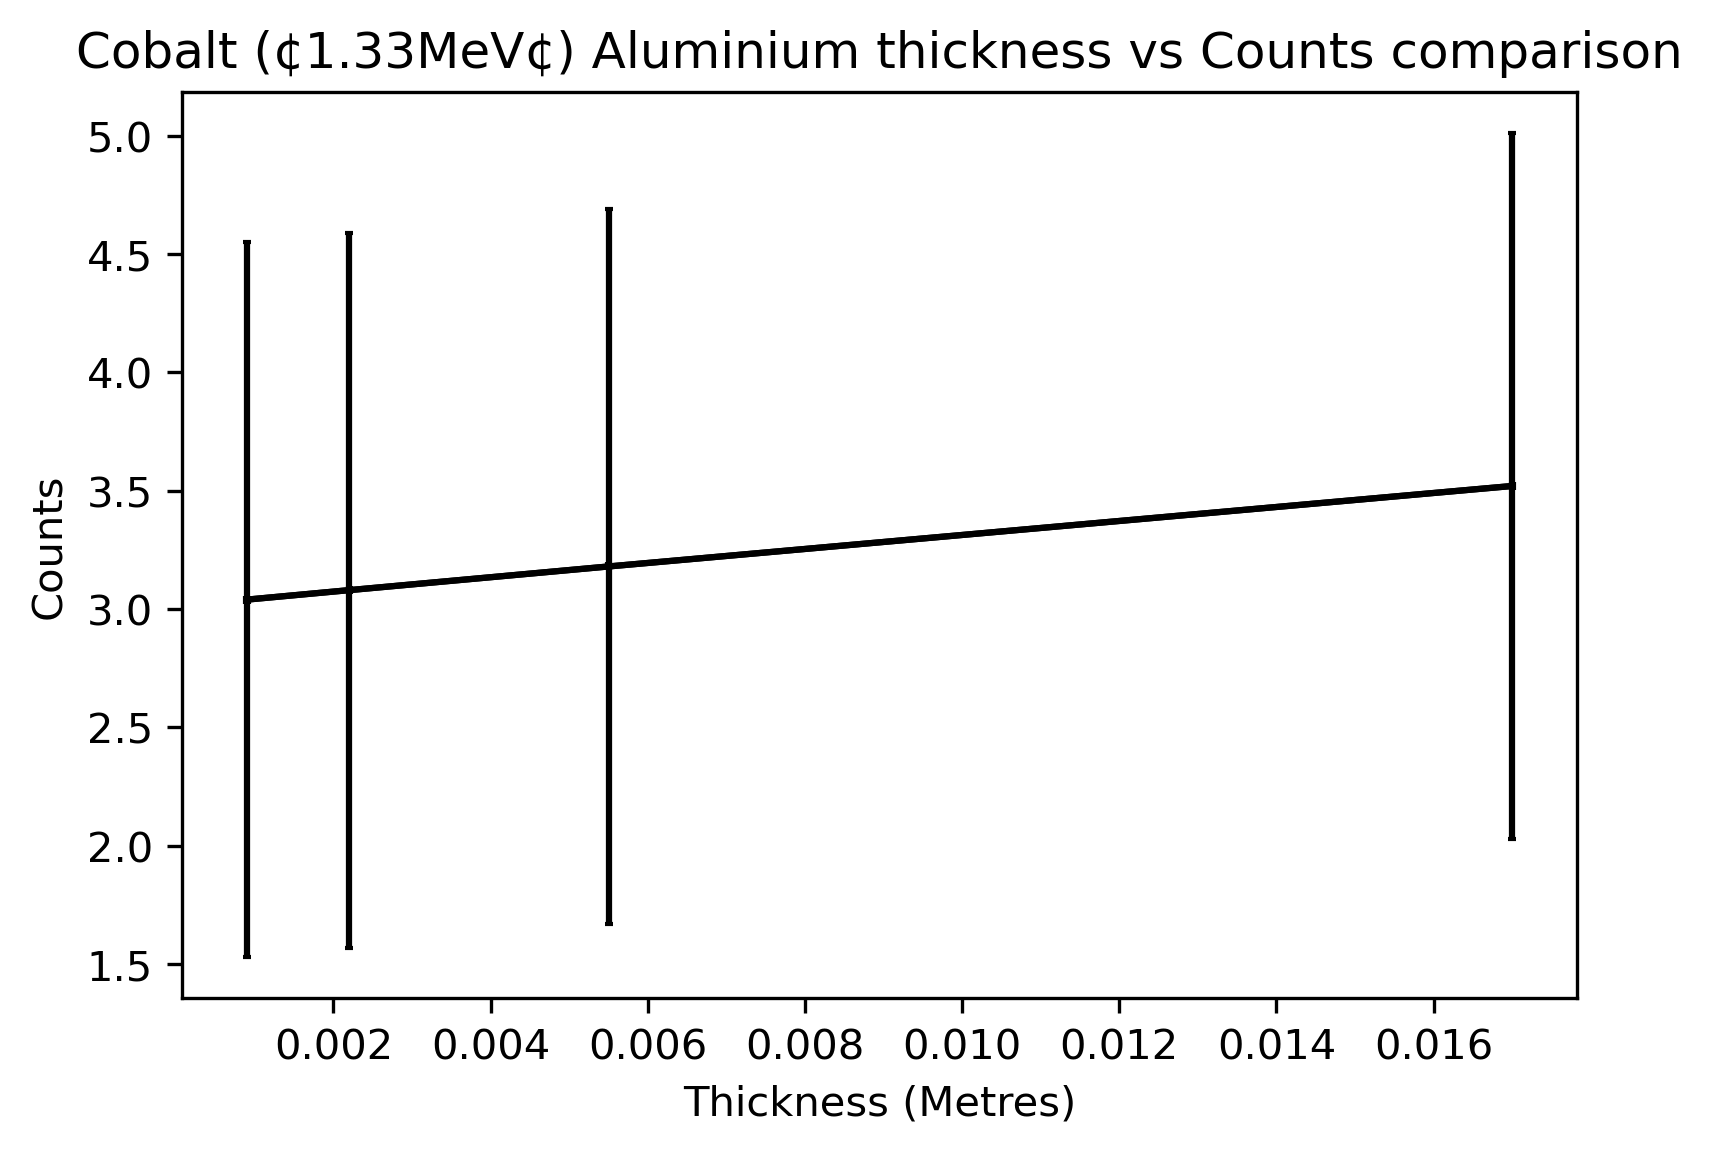
\includegraphics[scale=0.6]{Images/CobaltAlu133Final.png}
\caption{Graphical representation of \cref{Corrected Data} for Aluminium thickness in Cobalt (1.33 MeV).}
\label{Cobalt 133 Alu Final Counts}
\end{figure}
\end{multicols}

\begin{multicols}{2}
\begin{figure}[H]
\centering
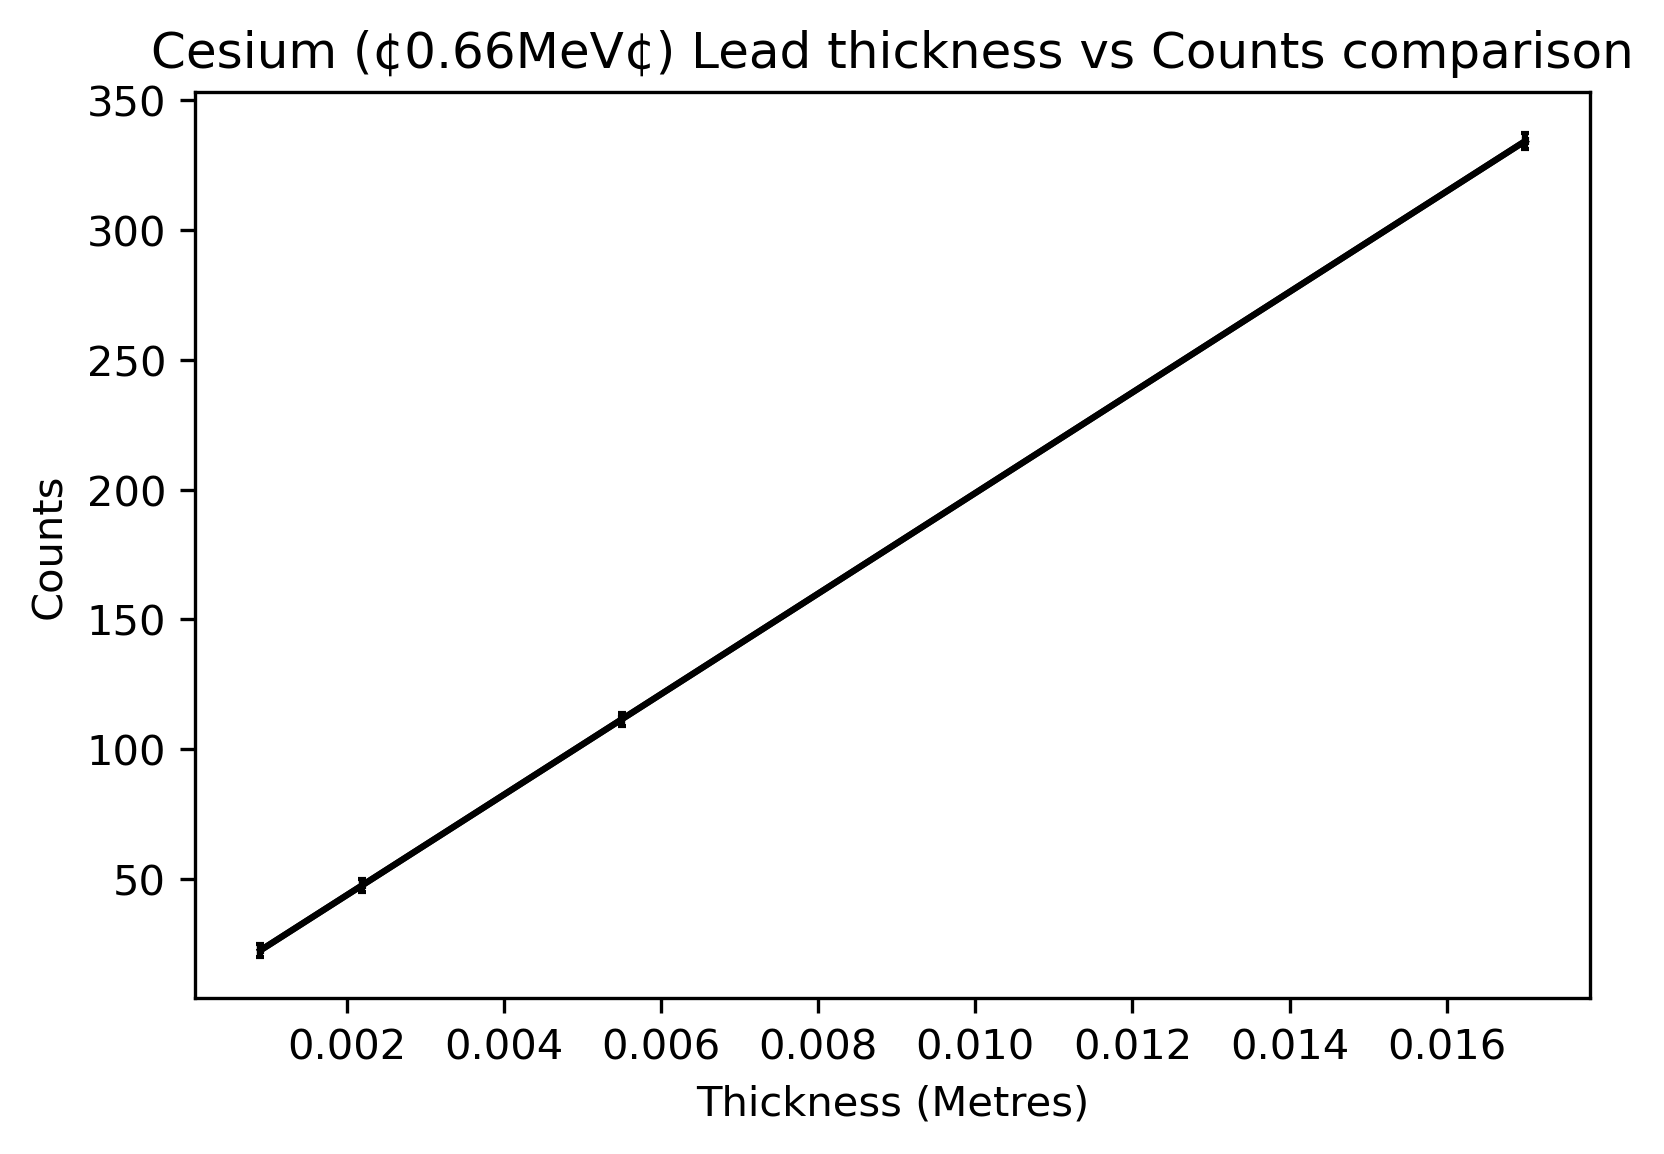
\includegraphics[scale=0.6]{Images/CesiumLead066Final.png}
\caption{Graphical representation of \cref{Corrected Data} for Lead thickness in Cesium (0.66 MeV).}
\label{Cesium 066 Lead Counts}
\end{figure}

\begin{figure}[H]
\centering
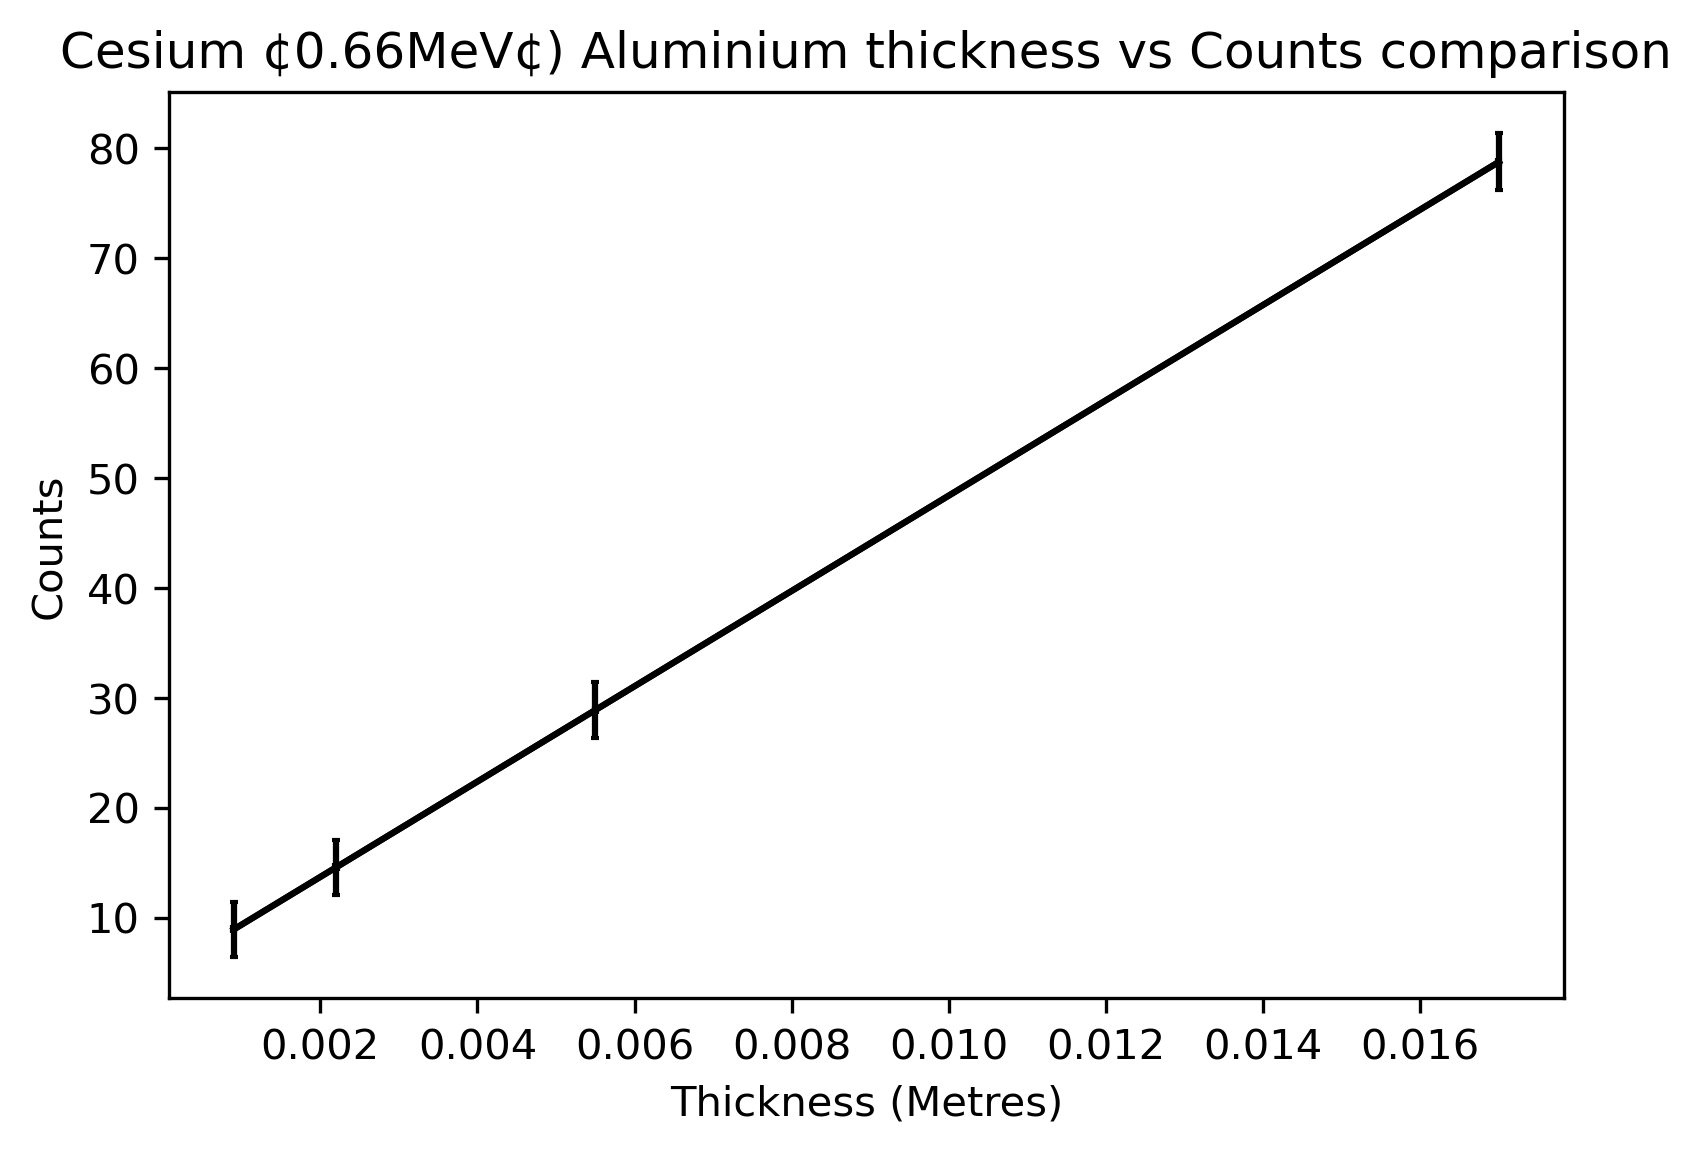
\includegraphics[scale=0.6]{Images/CesiumAlu066Final.png}
\caption{Graphical representation of \cref{Corrected Data} for Aluminium thickness in Cesium (0.66 MeV).}
\label{Cesium 066 Alu Counts}
\end{figure}
\end{multicols}

By analysing these graphs it can be seen that there is a significant linear relationship in regard to the Cesium source and both the lead and aluminium materials with minor error values. Whereas the Cobalt source shows again significant linear similarities with both materials and both of the Cobalt's energy levels but yet the error values are too great to deem a linear relationship between them.

%---------------------------------------------------------------------------
%	DISCUSSION
%---------------------------------------------------------------------------
\newpage
\section{Discussion}
\label{Disscussion Section}

Within this experiment there were many values of raw data each with different errors, where the overstated error bars in the Lead graphs of corrected results seem to large, large enough to not accurately state a definitive result. The linear attenuation co-efficient calculation could be to blame as the values for cesium are to far apart. \\

But the initial counts show that lead absorbs gamma rays better than aluminium regardless of the radioactive source which is backed with the knowledge that lead is used in nuclear reactors due to this effect it was anticipated that lead would have low gamma rays counts against the aluminium but also as the thickness of lead increased. More radioactive sources would have been useful to solidify this conclusion and possibly more different types of materials that could exploring the penetration of the gamma rays.

%---------------------------------------------------------------------------
%	CONCLUSION
%---------------------------------------------------------------------------
\section{Conclusion}
\label{Conclusion Section}

In conclusion, this experiment proved that one material is better than another at absorbing gamma rays and this is due to their different atomic layout, measuring the penetrated gamma ray counts for different thicknesses proved this and shows how gamma rays travel though the different materials. The intensities for both the Cobalt and Cesium remained linear showing a direct correlation between the gamma ray counts and the various thicknesses. Now looking back at the aims of this experiment the energy resolution was found by identifying key features of the spectra as the radioactive sources were measured, though the calculated values for the liner and mass attenuation co-efficient caused the final corrected error values to be too big this experiment has met all of its aims.

%---------------------------------------------------------------------------
%	APPENDIX
%---------------------------------------------------------------------------
\newpage
\section{Lab Book}
\label{Lab BookSection}

\begin{figure}[H]
\centering
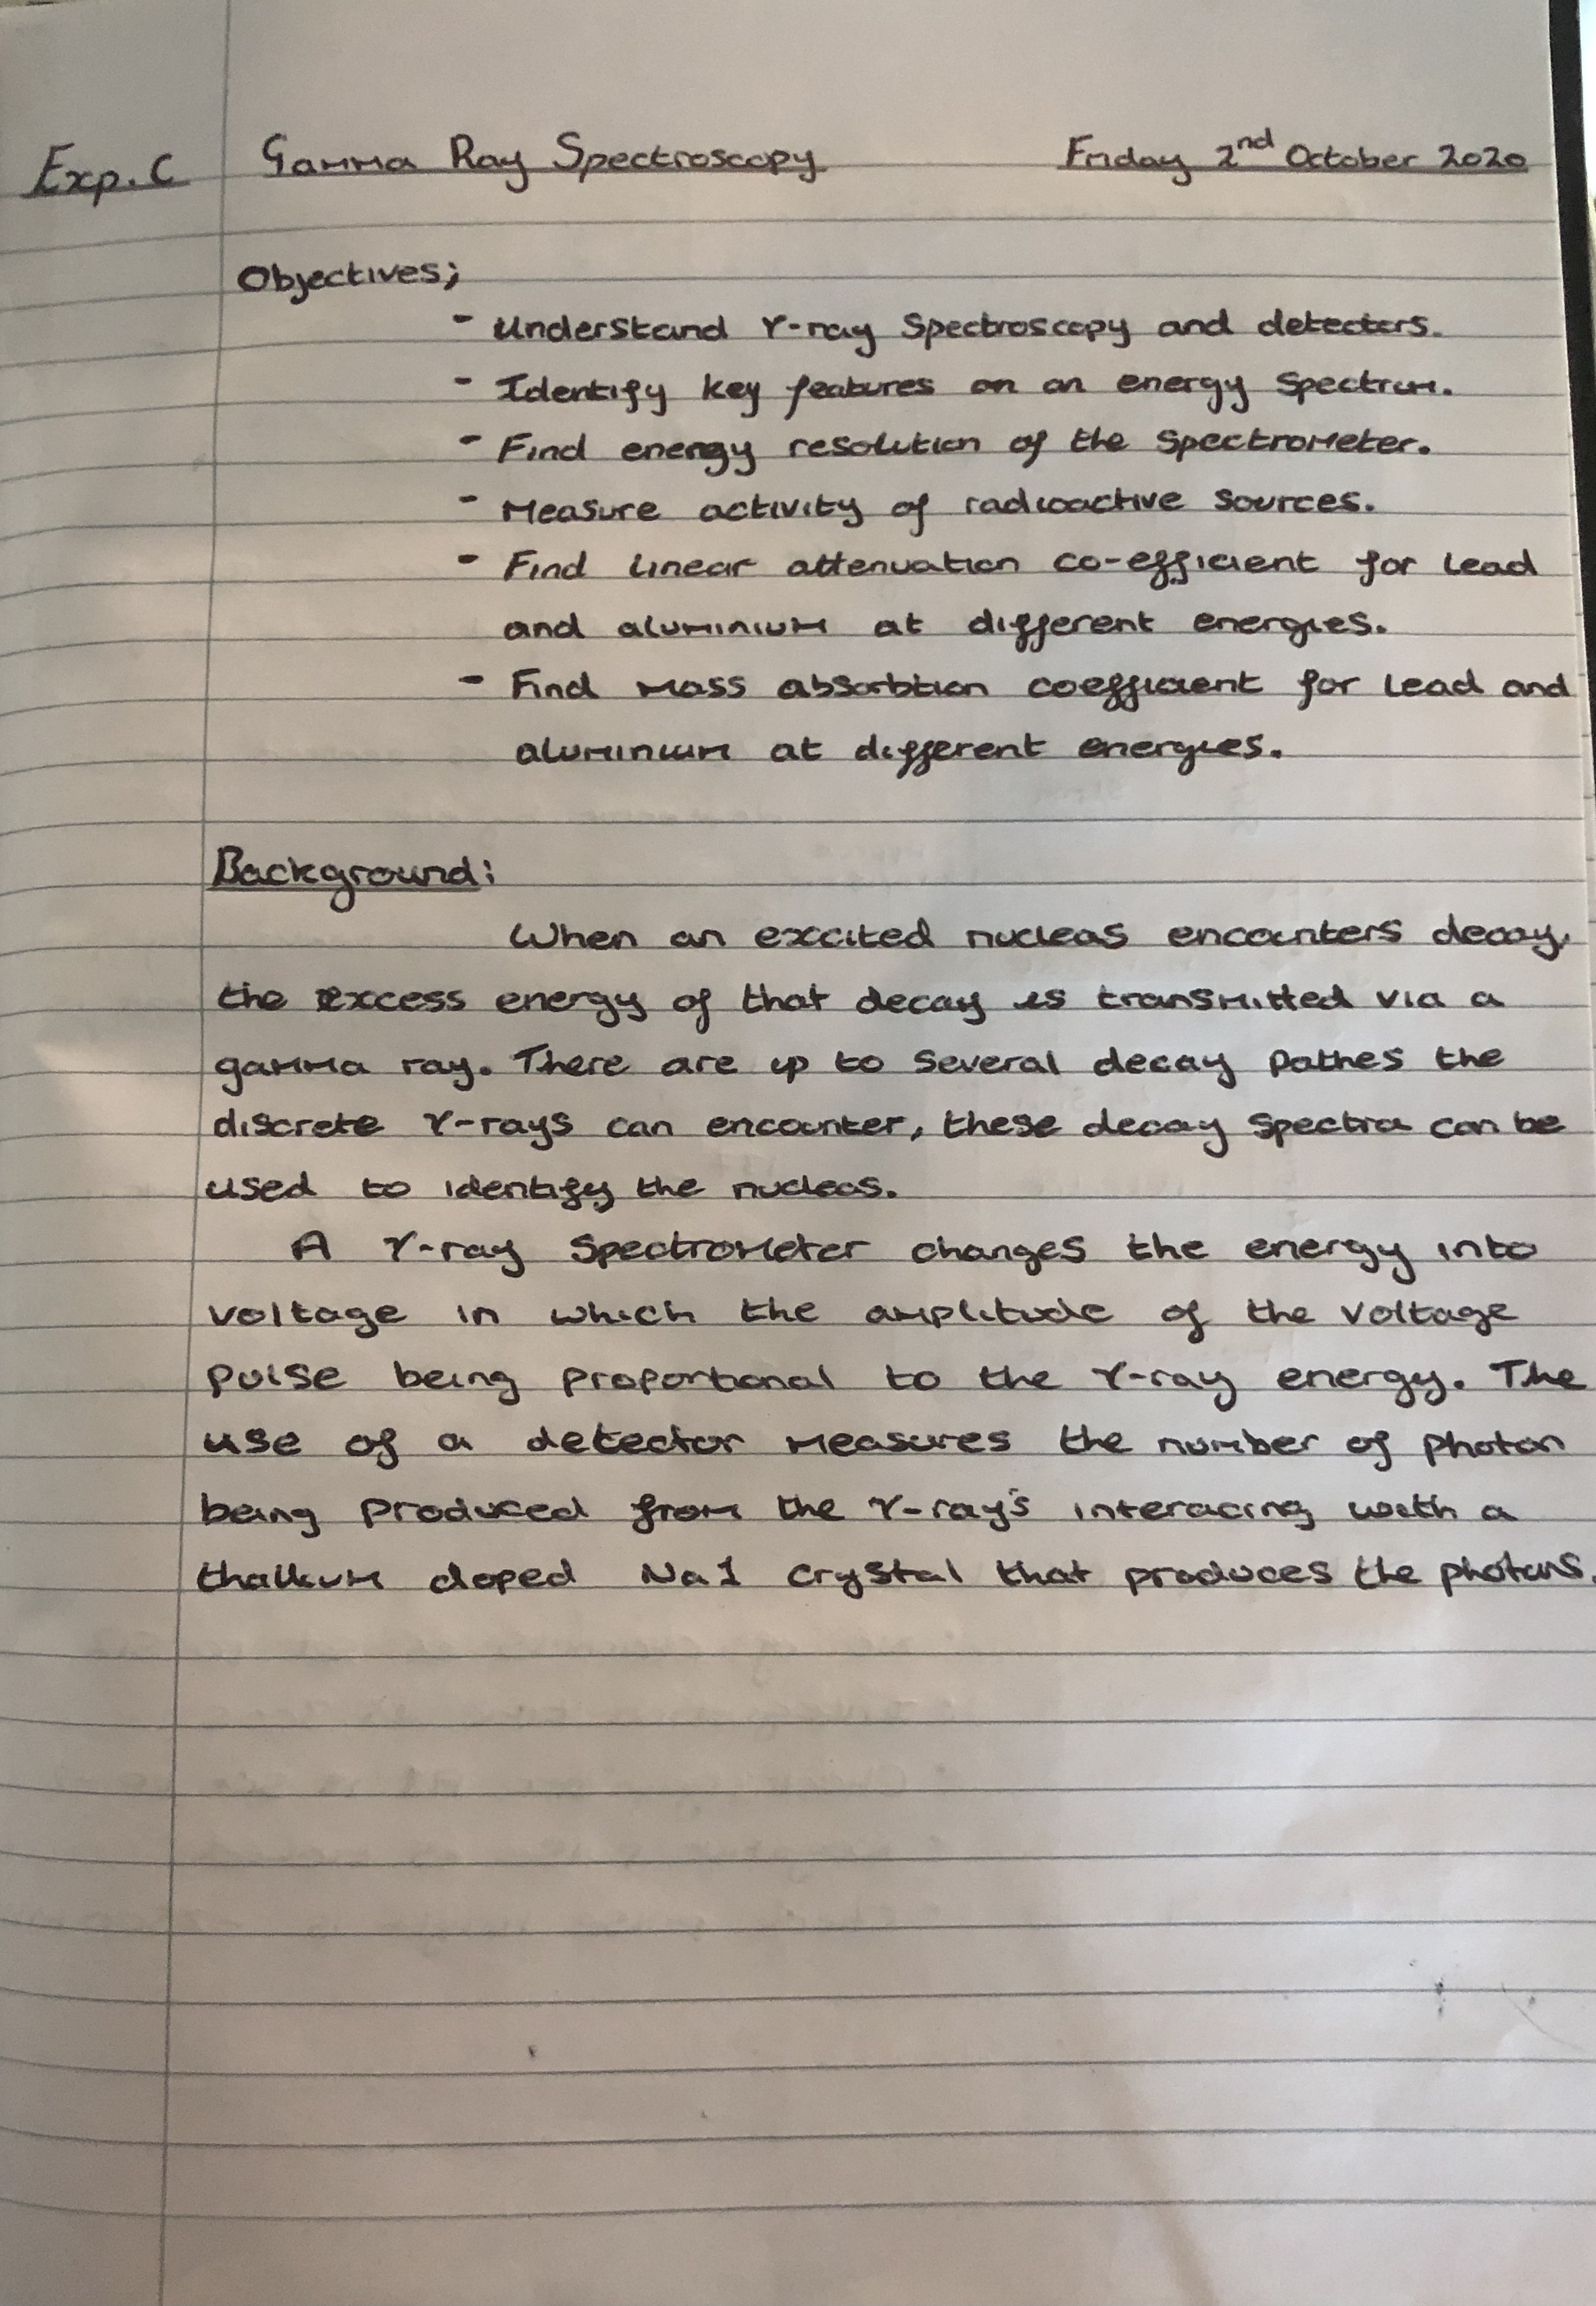
\includegraphics[scale=0.18]{Images/IMG_0330.JPG}
\end{figure}
\newpage
\begin{figure}[H]
\centering
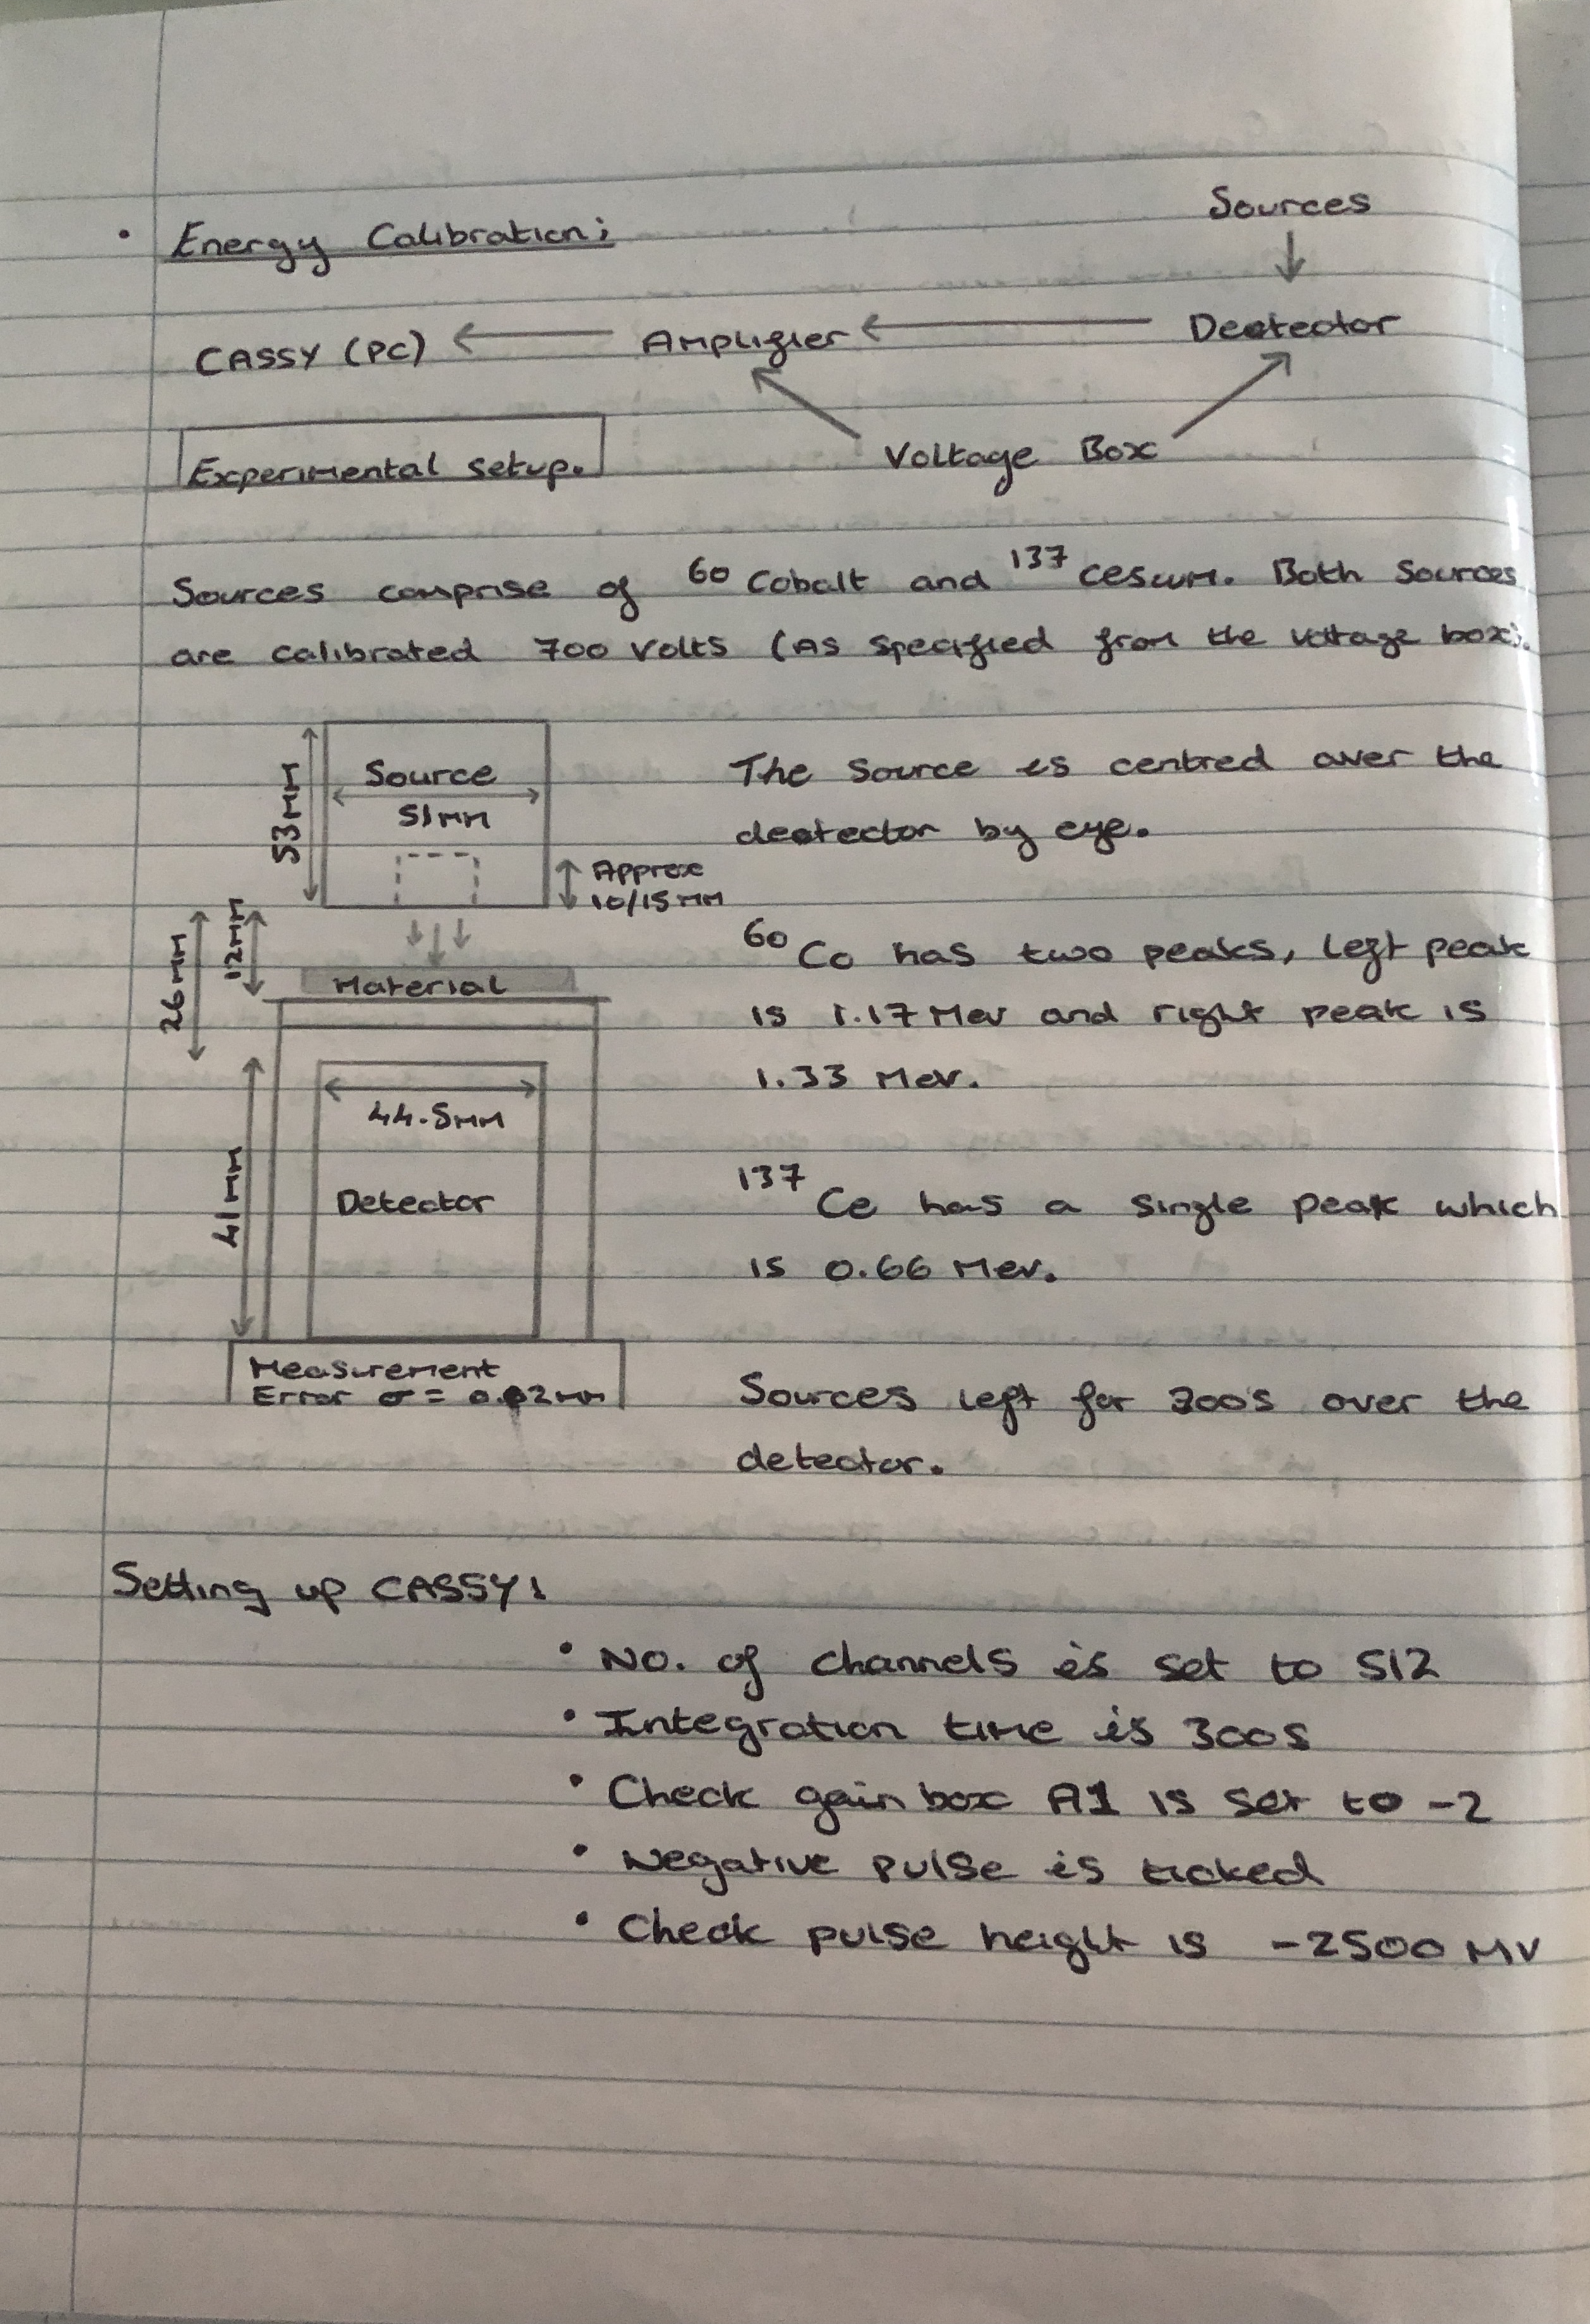
\includegraphics[scale=0.175]{Images/IMG_0331.JPG}
\end{figure}
\newpage
\begin{figure}[H]
\centering
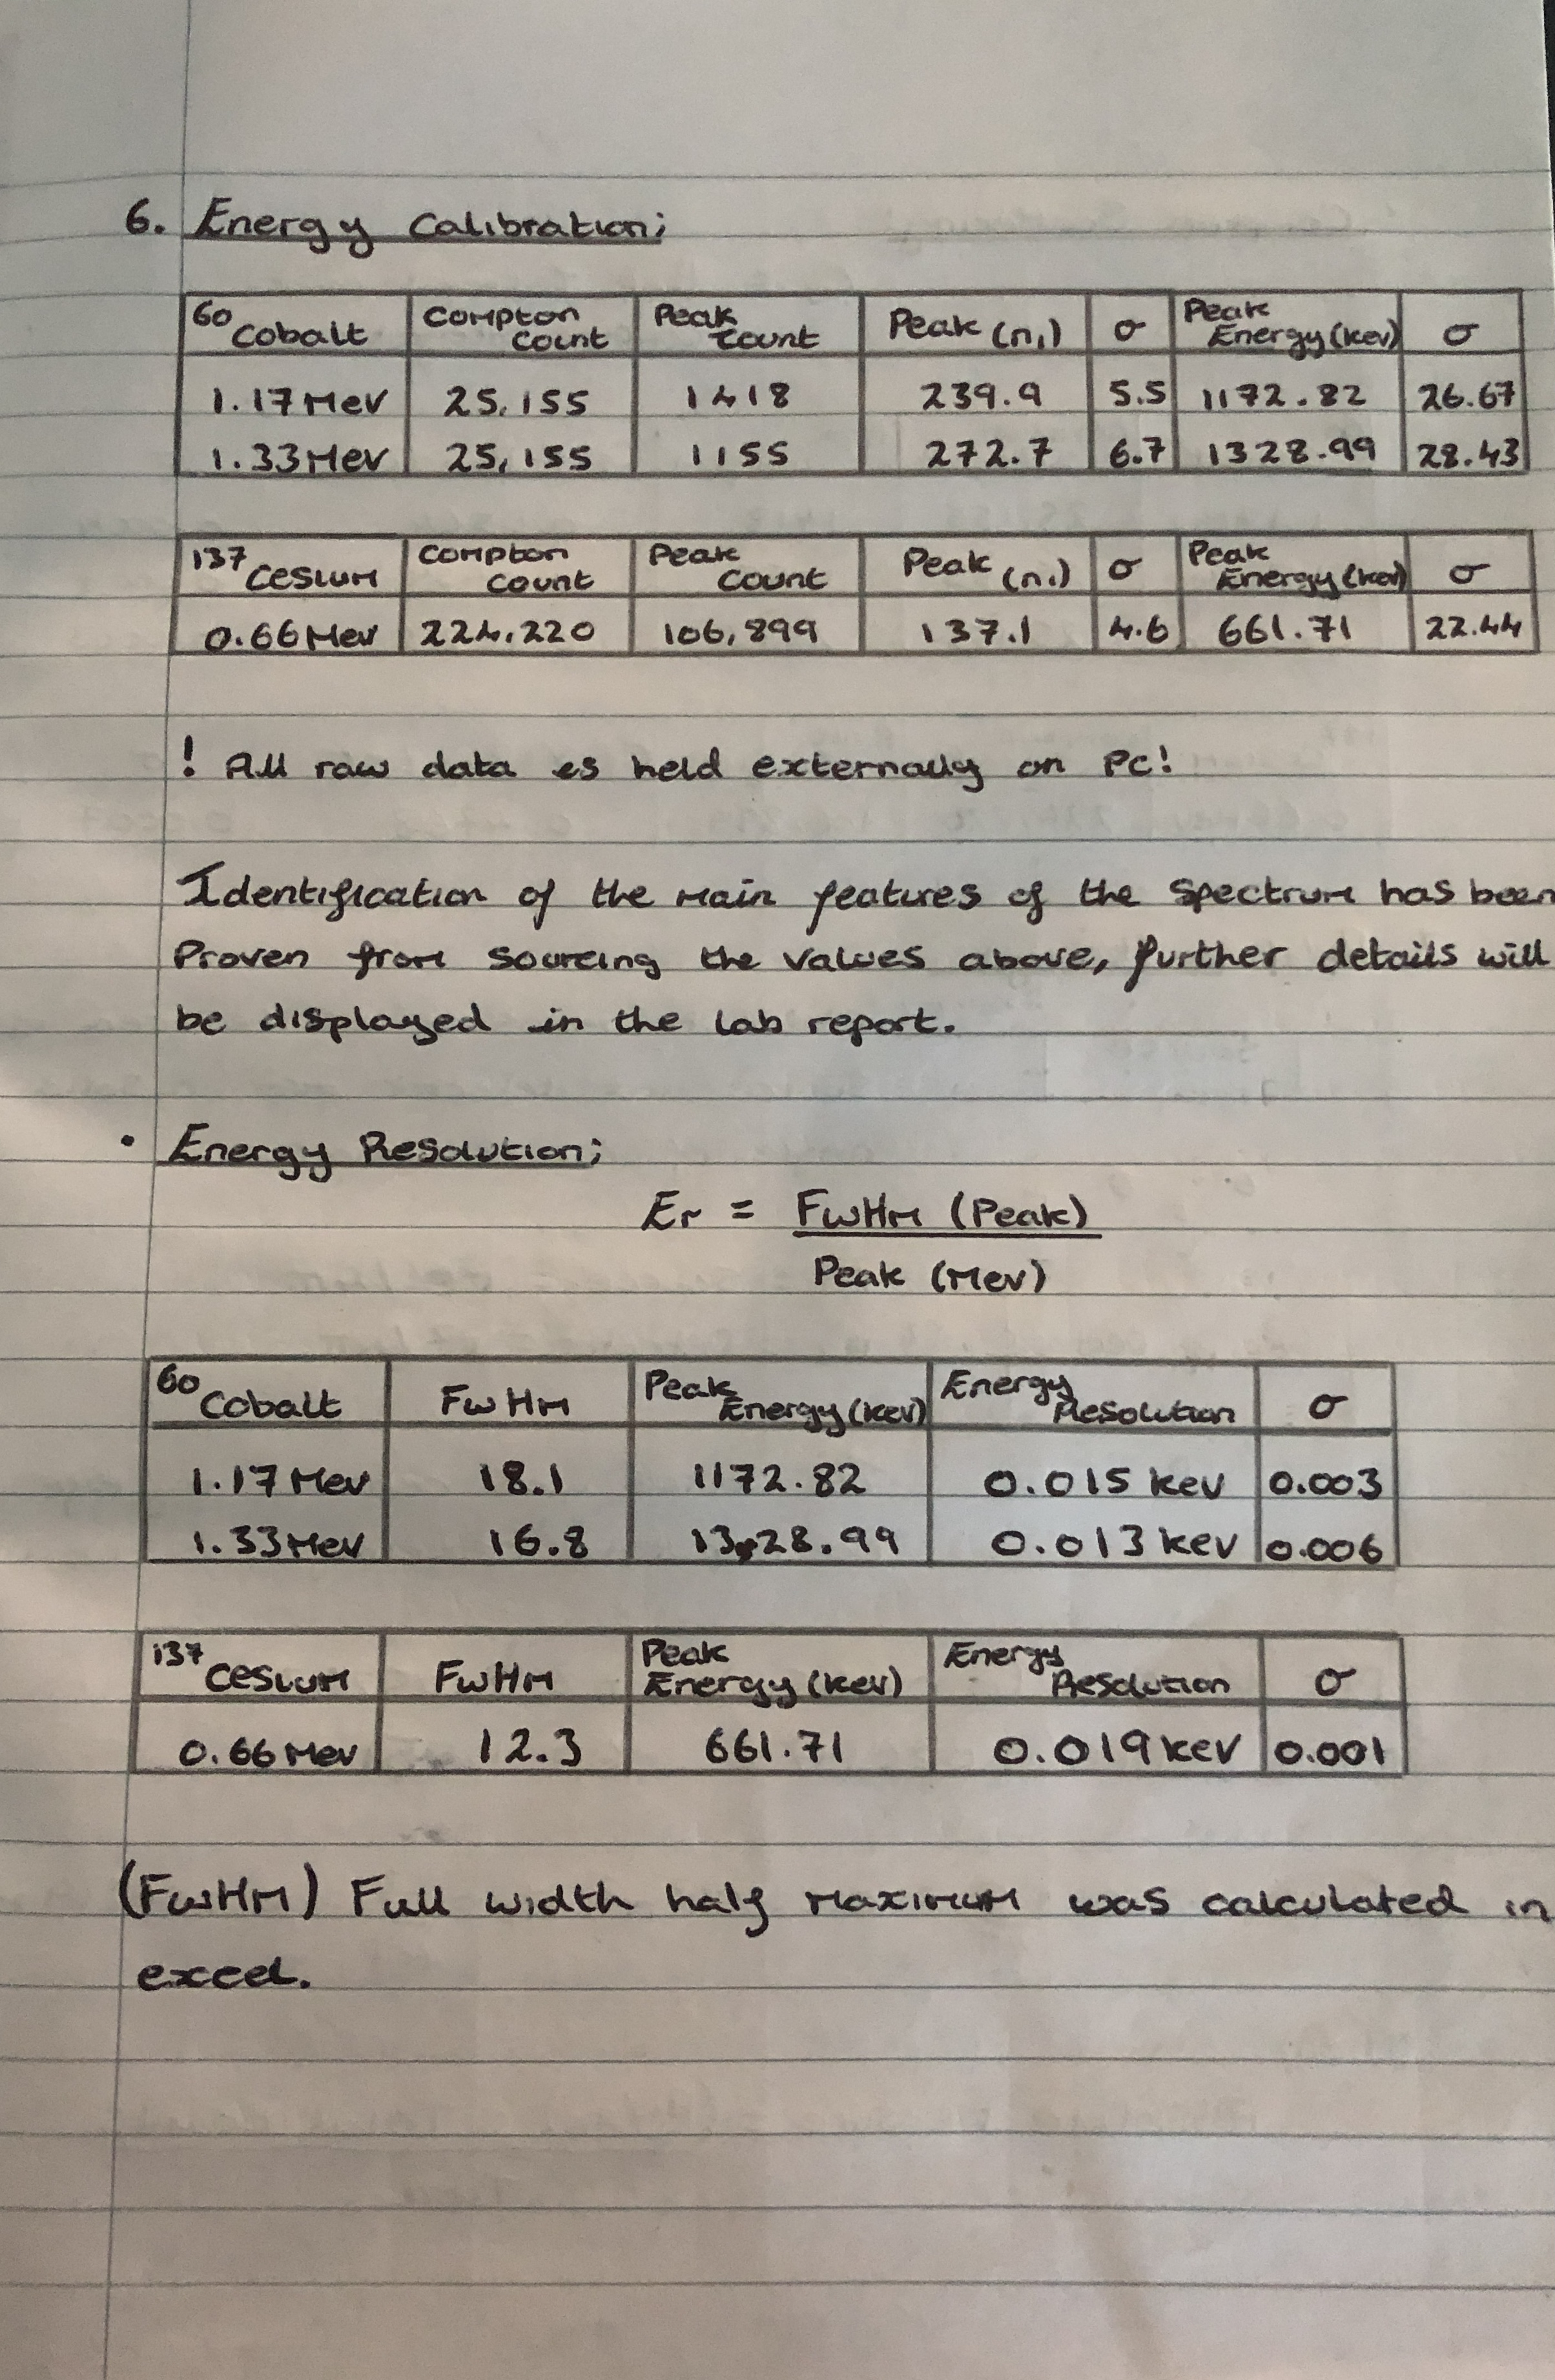
\includegraphics[scale=0.175]{Images/IMG_0332.JPG}
\end{figure}
\newpage
\begin{figure}[H]
\centering
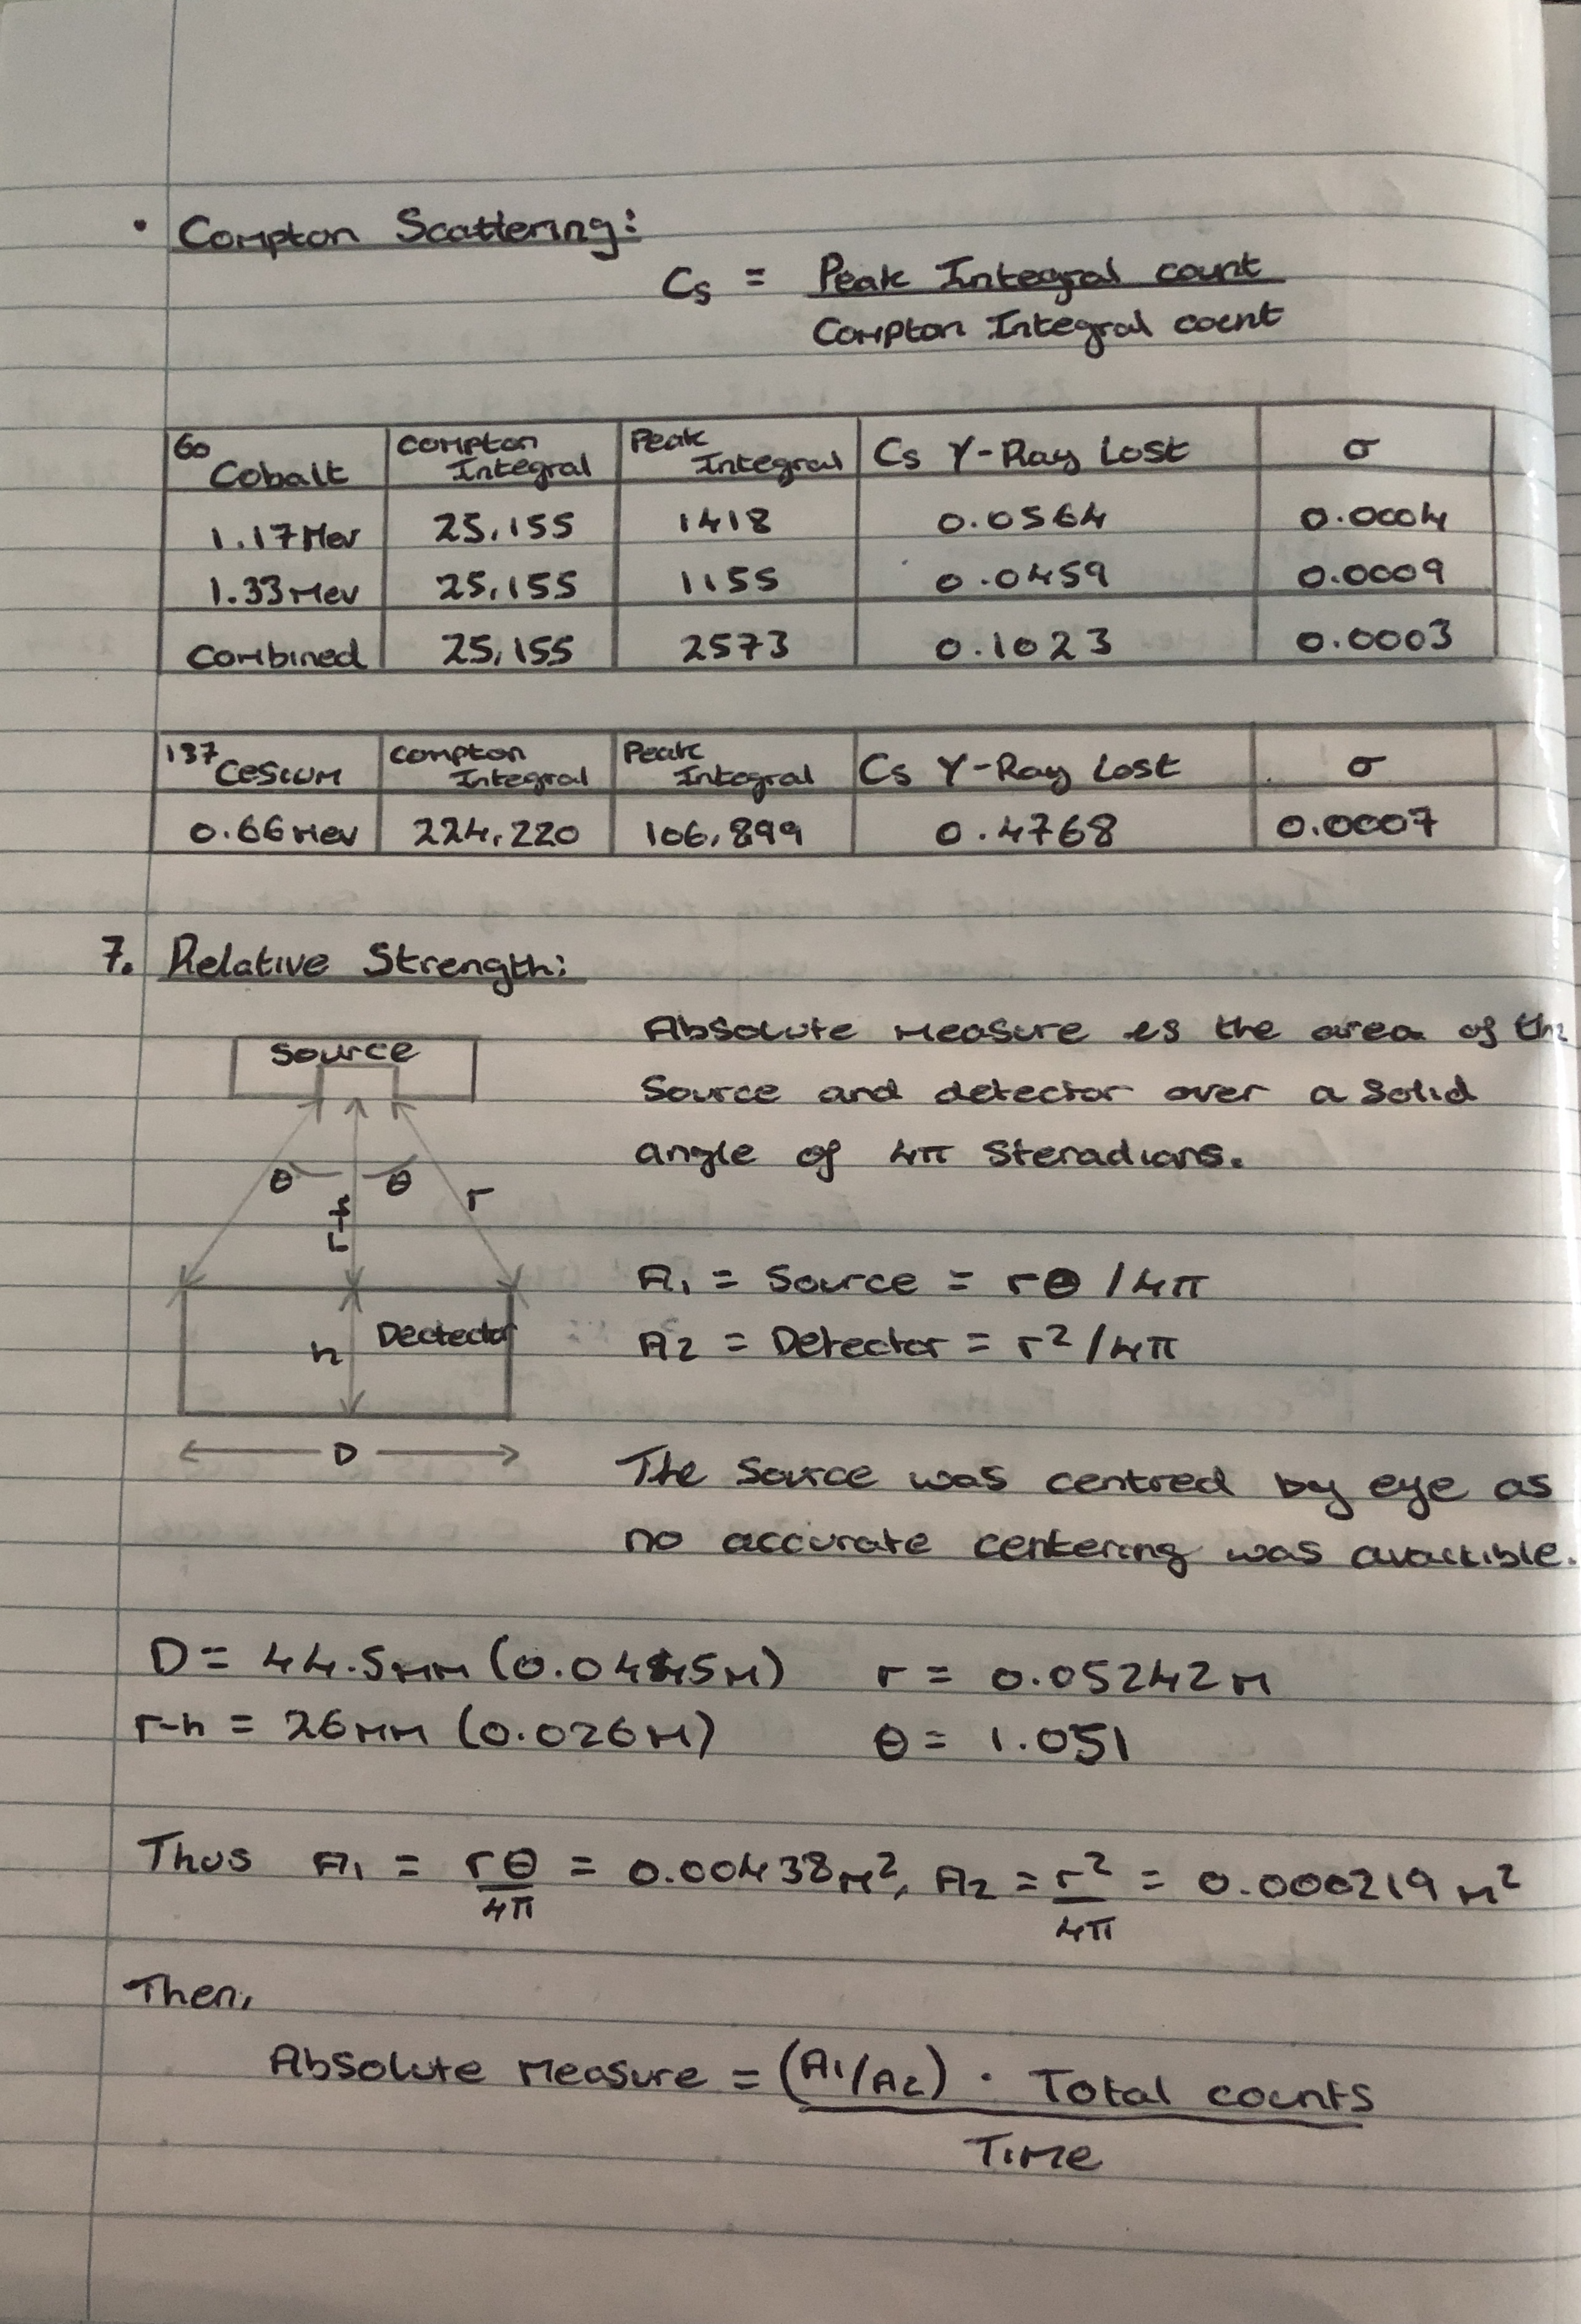
\includegraphics[scale=0.175]{Images/IMG_0333.JPG}
\end{figure}
\newpage
\begin{figure}[H]
\centering
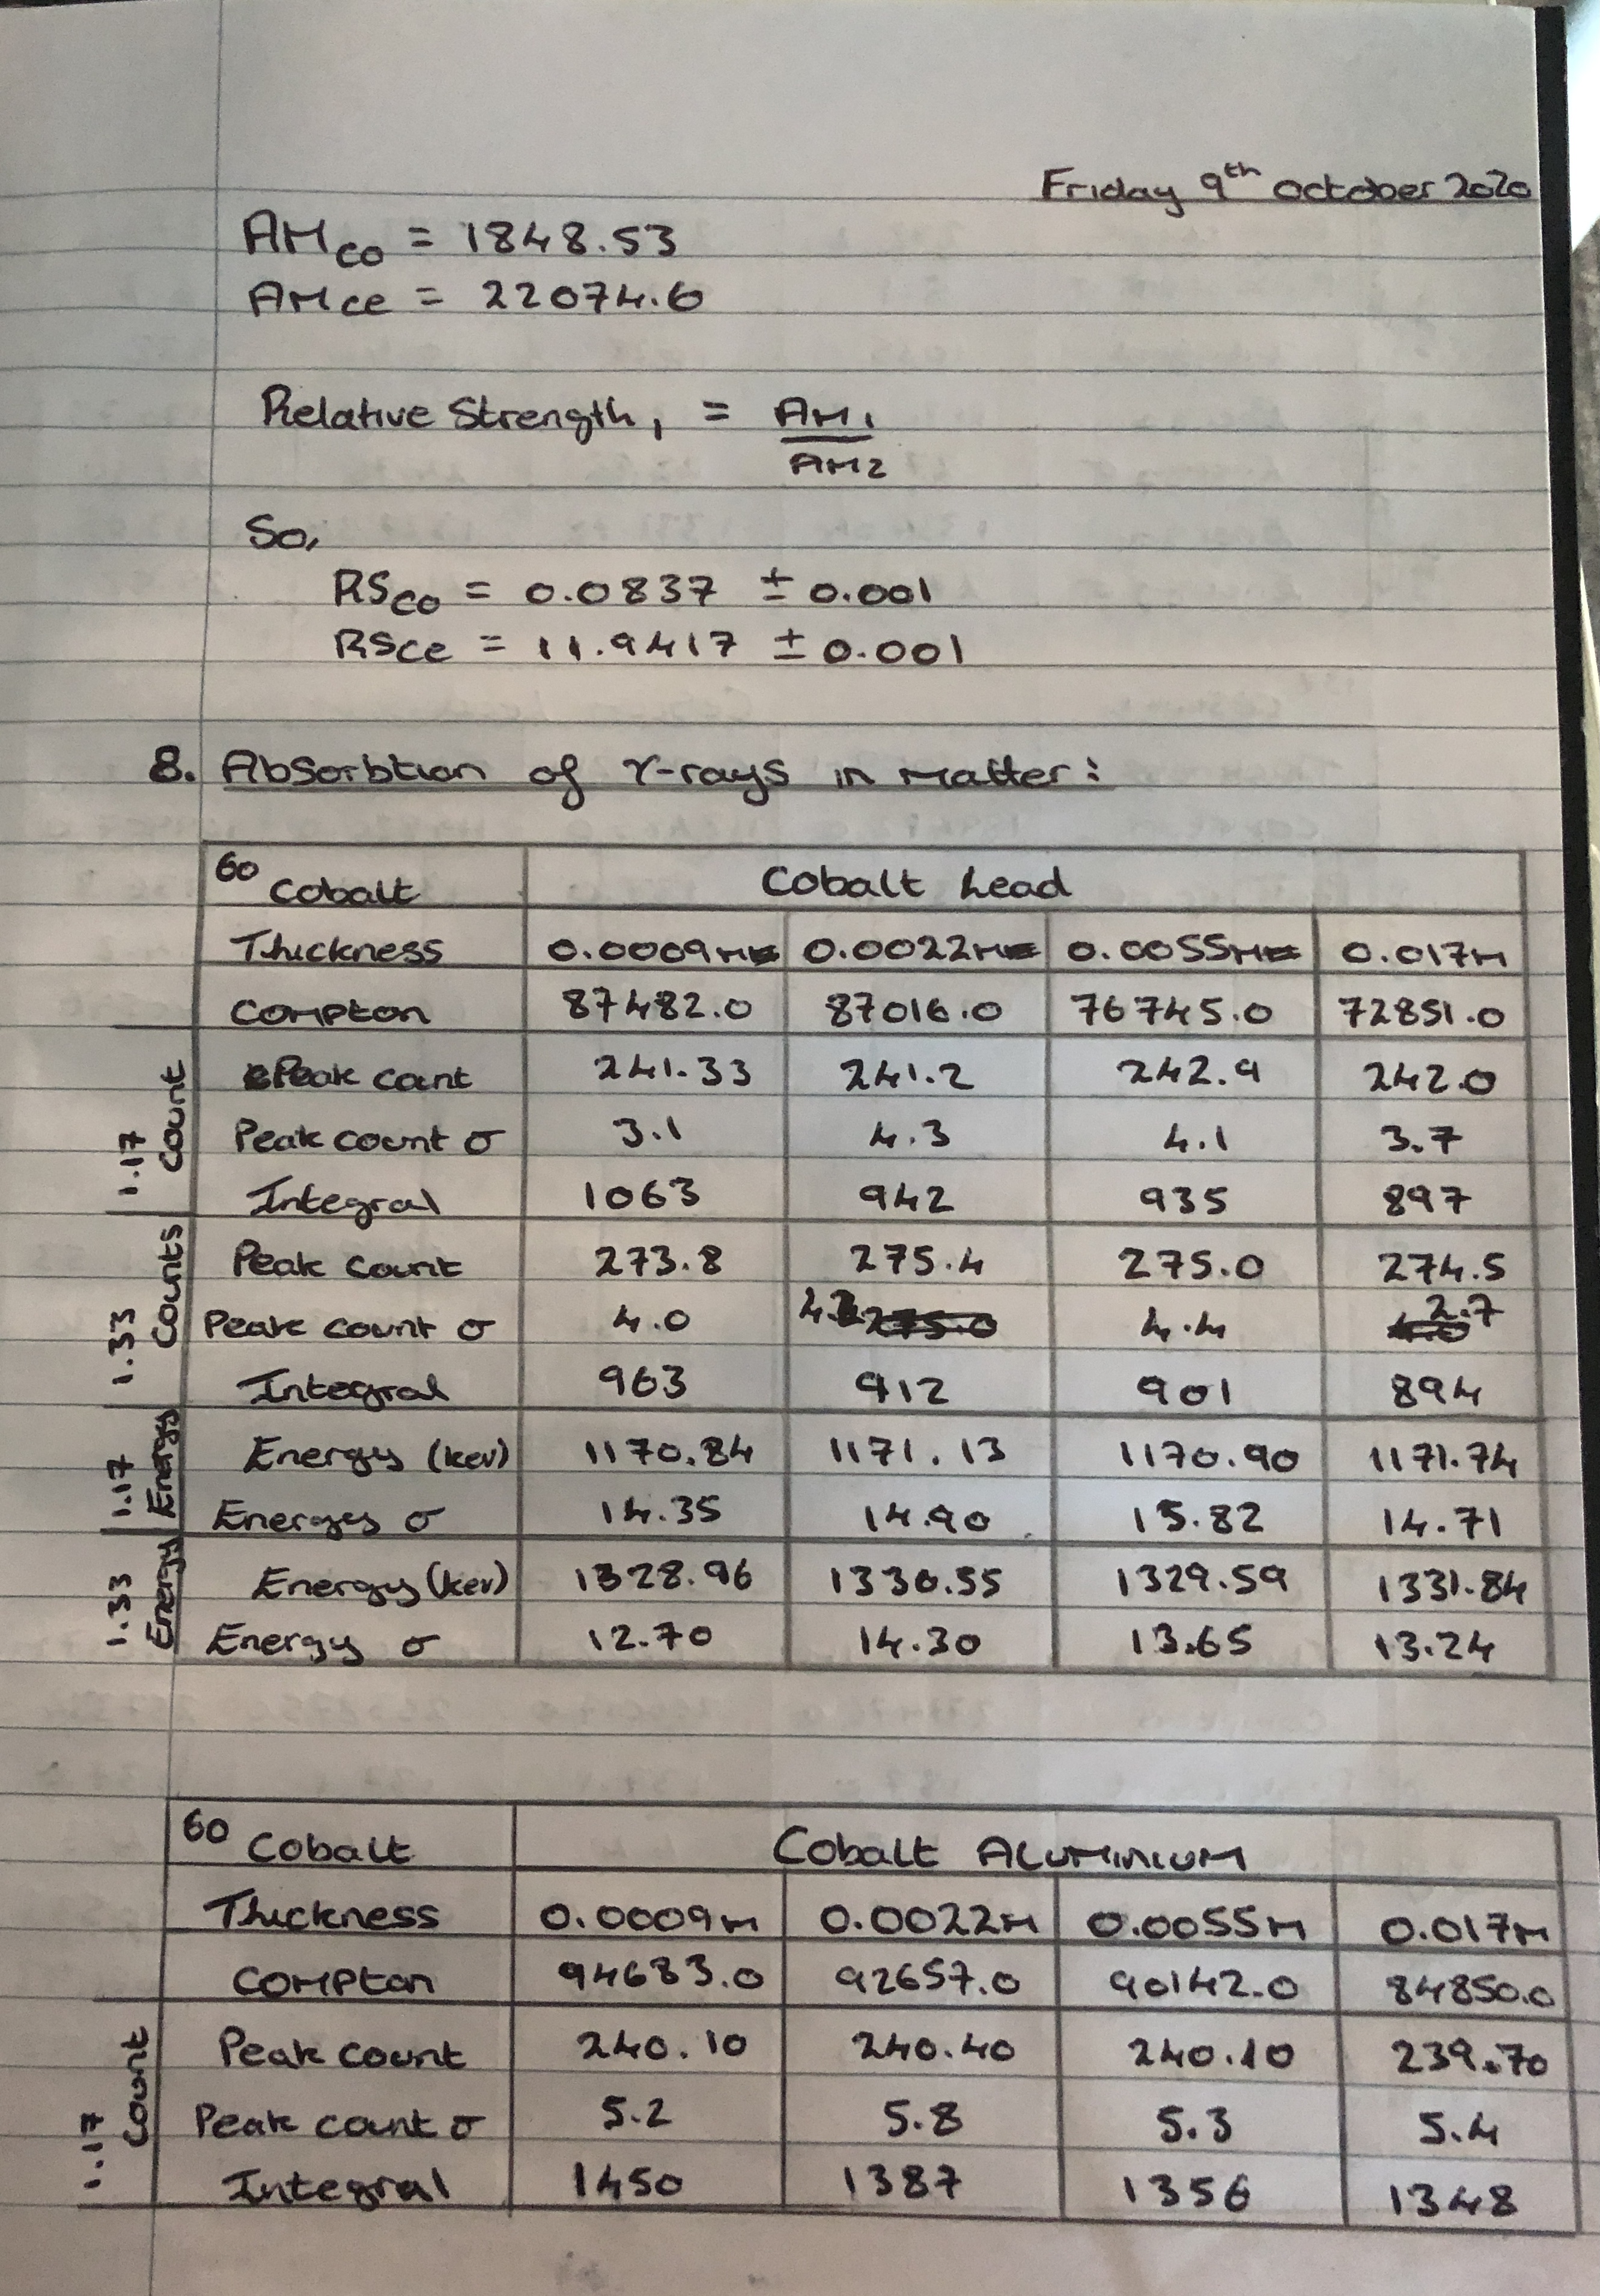
\includegraphics[scale=0.17]{Images/IMG_0334.JPG}
\end{figure}
\newpage
\begin{figure}[H]
\centering
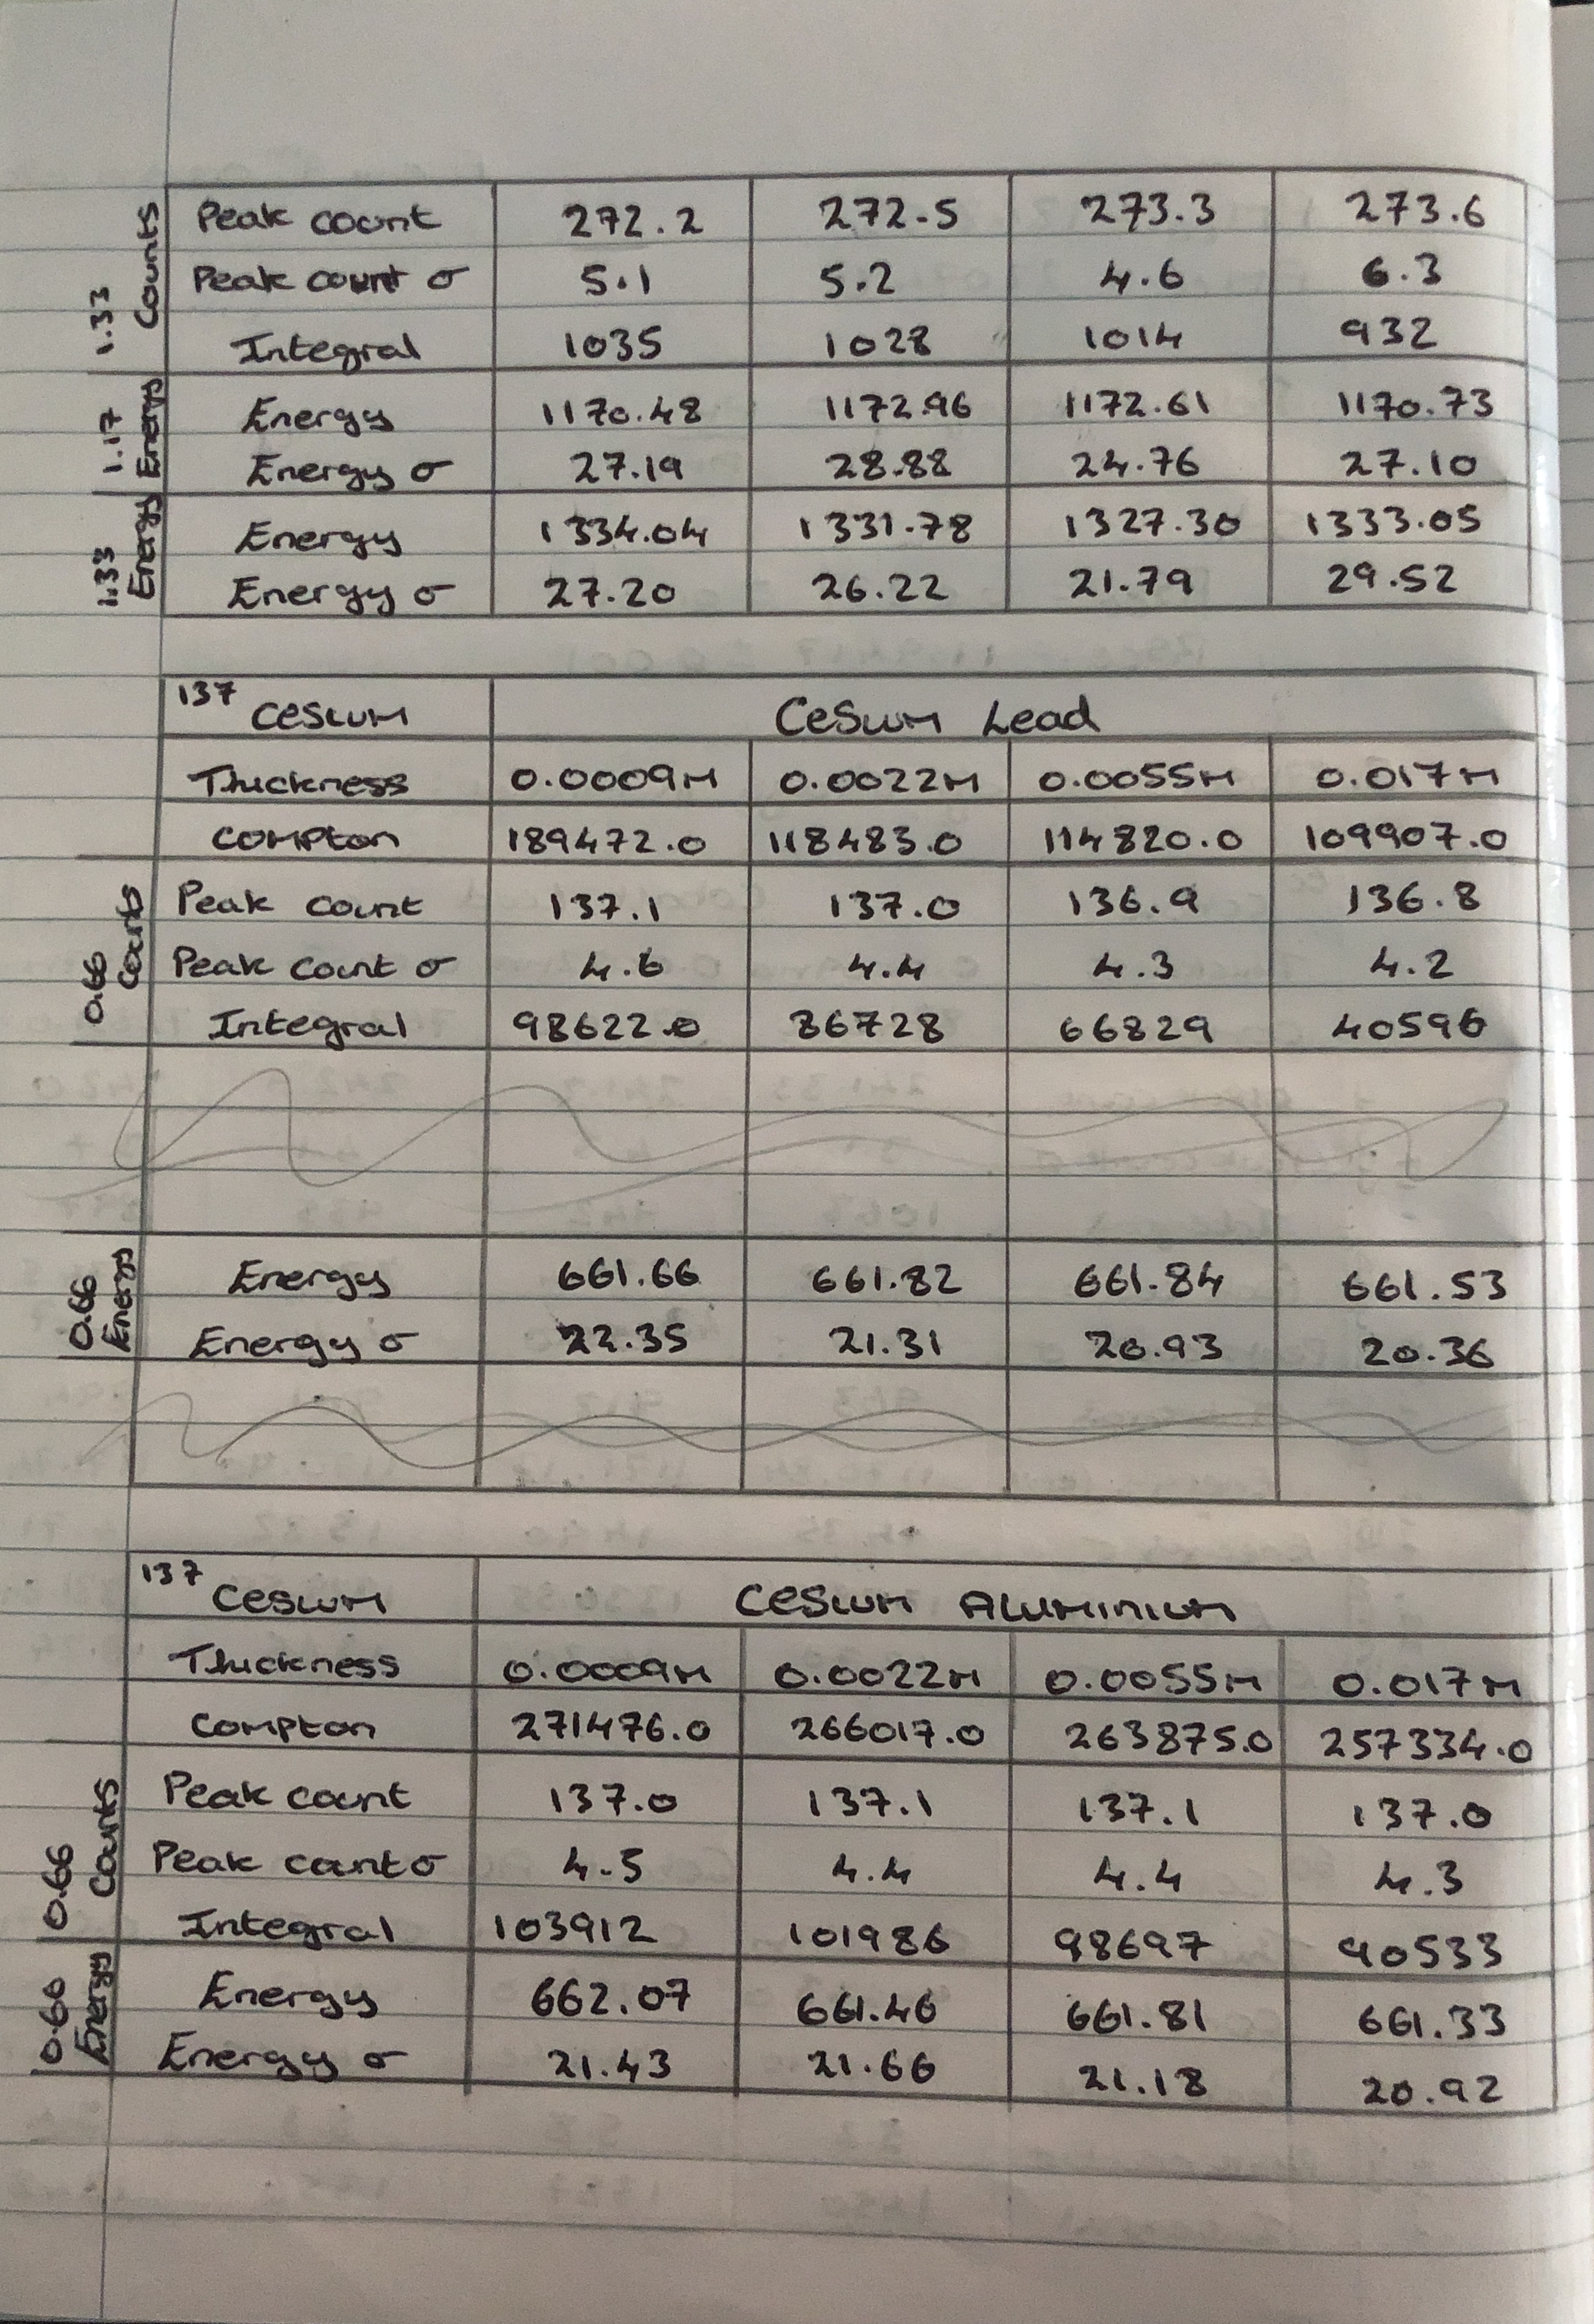
\includegraphics[scale=0.175]{Images/IMG_0335.JPG}
\end{figure}
\newpage
\begin{figure}[H]
\centering
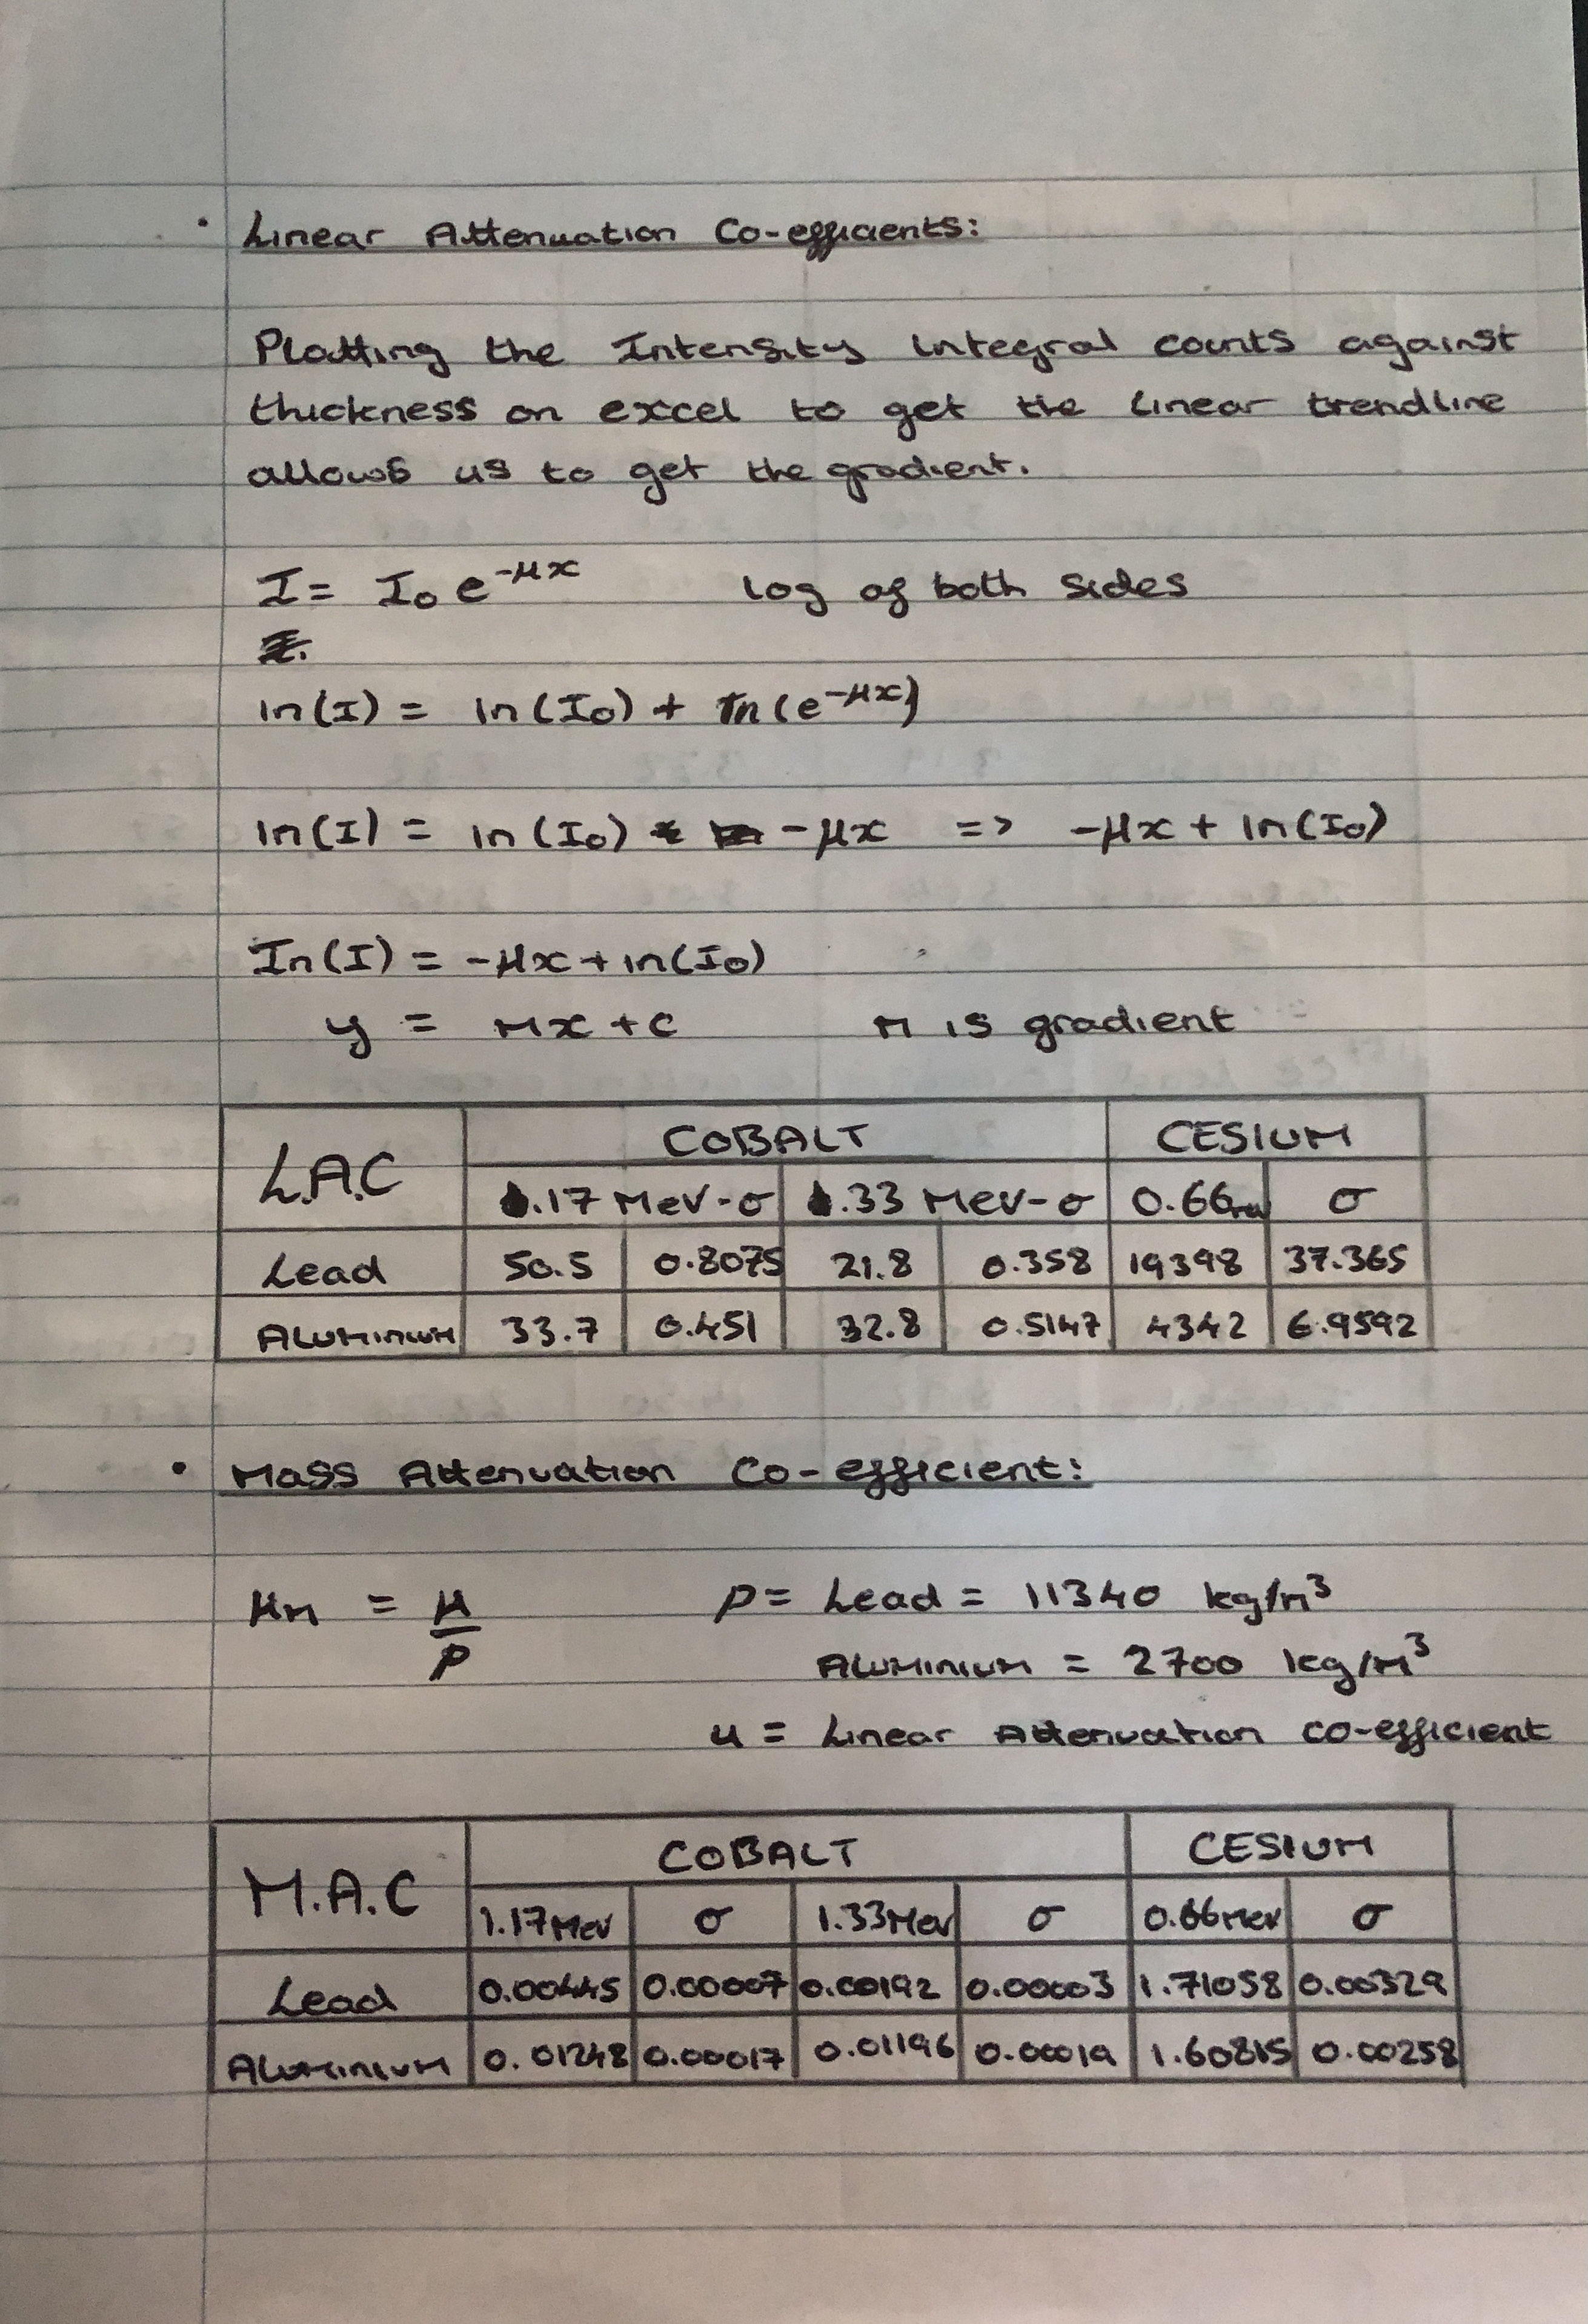
\includegraphics[scale=0.17]{Images/IMG_0336.JPG}
\end{figure}
\newpage
\begin{figure}[H]
\centering
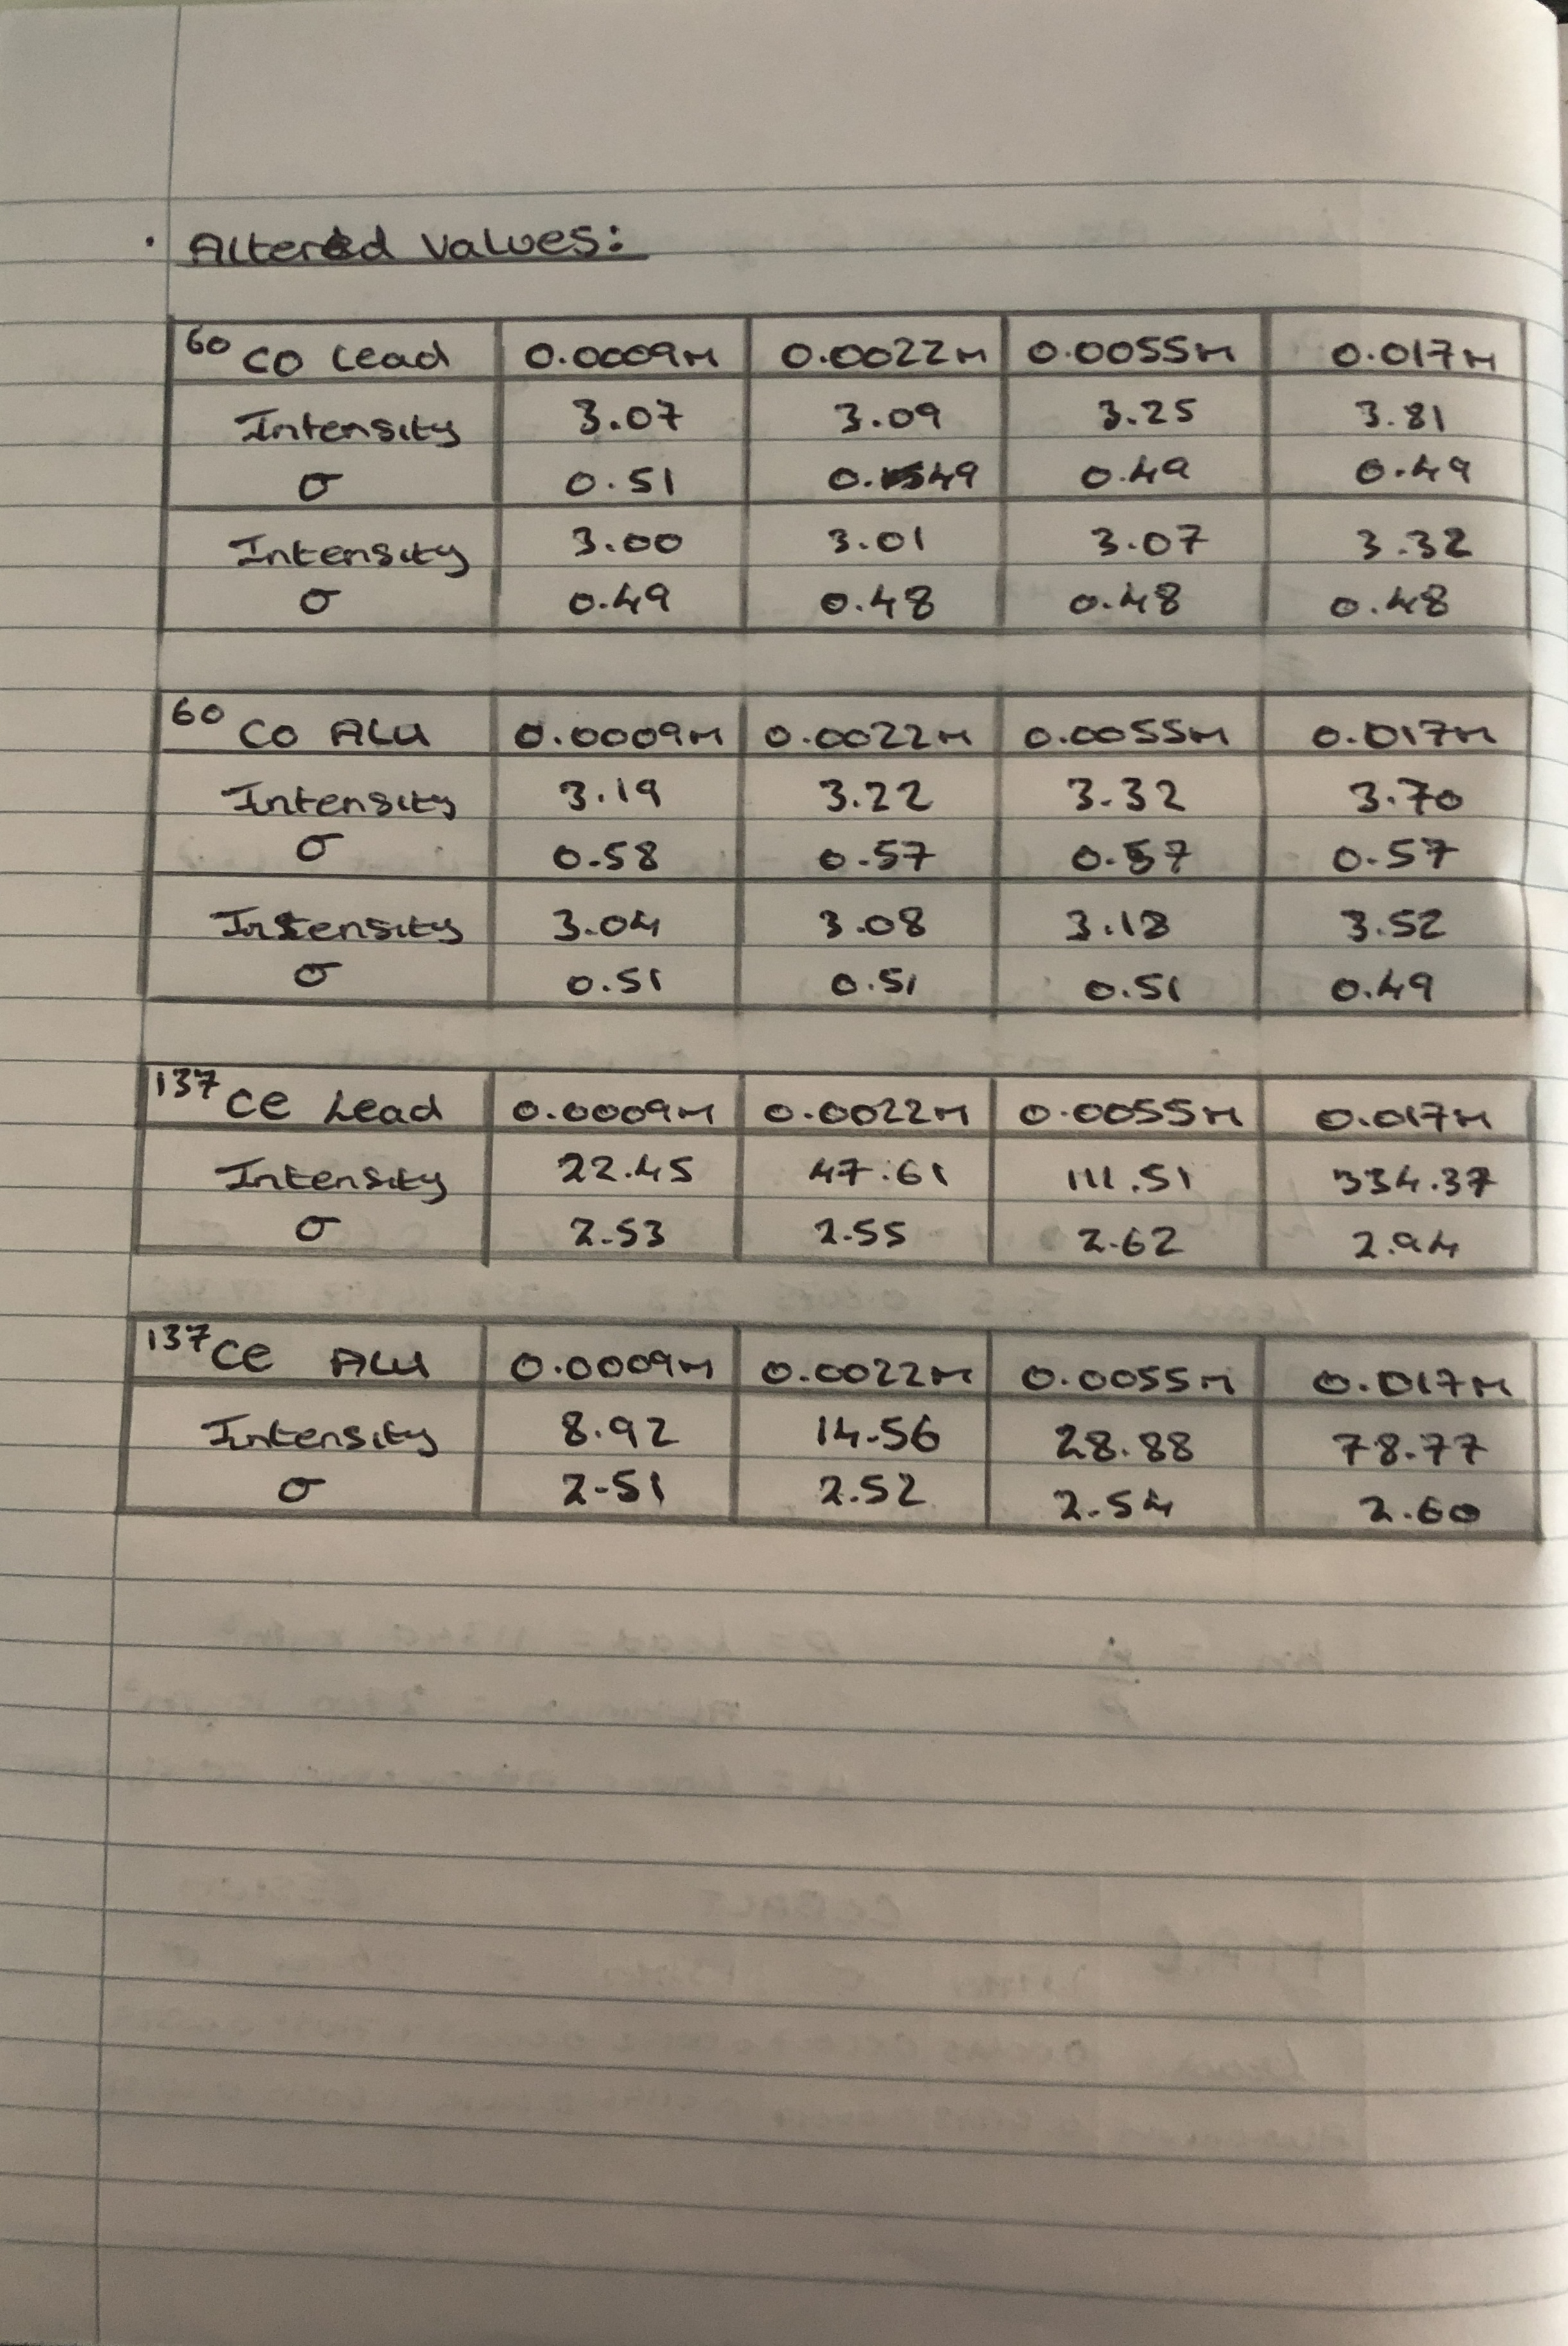
\includegraphics[scale=0.18]{Images/IMG_0337.JPG}
\end{figure}
%---------------------------------------------------------------------------
%	REFERENCES
%---------------------------------------------------------------------------
\bibliographystyle{plain}
\bibliography{Report/mybib}
\end{document}